\documentclass[a4paper,12pt,headsepline]{scrartcl}
%Variablen welche innerhalb der gesamten Arbeit zur Verfügung stehen sollen
\newcommand{\titleDocument}{Bachelor- / Masterarbeit}
\newcommand{\subjectDocument}{im Studiengang <Studiengang>}
\usepackage{graphicx}
\usepackage[right]{eurosym}
\usepackage[utf8]{inputenc}
\usepackage[T1]{fontenc}
\usepackage{lmodern}
\usepackage{fix-cm}
\usepackage{longtable}
\usepackage{geometry}
\geometry{left=3.5cm, right=2cm, top=2.5cm, bottom=2cm}
\usepackage{fancybox}
\usepackage[hyphens,obeyspaces,spaces]{url}
\usepackage{color}
\usepackage[bookmarksnumbered,pdftitle={\titleDocument},hyperfootnotes=false]{hyperref} 
\usepackage{fancyhdr} %Paket laden
\pagestyle{fancy} %eigener Seitenstil
\usepackage[export]{adjustbox}
\usepackage{tabularx}
%\bibliographystyle{stylename}

%CUSTOM PACKAGES
\usepackage{soul}


\fancyhf{} %alle Kopf- und Fußzeilenfelder bereinigen
\fancyhead[L]{\nouppercase{\leftmark}} %Kopfzeile links
\fancyhead[C]{} %zentrierte Kopfzeile
\fancyhead[R]{\thepage} %Kopfzeile rechts
\renewcommand{\headrulewidth}{0.4pt} %obere Trennlinie

\usepackage{array}
\bibliographystyle{acm}
\renewcommand{\sc}{\textsc}



\frenchspacing
\usepackage{setspace}
\usepackage{capt-of}
\usepackage{makeidx}
\usepackage{listings}
\lstset{numbers=left, numberstyle=\tiny, numbersep=5pt, keywordstyle=\color{black}\bfseries, stringstyle=\ttfamily,showstringspaces=false,basicstyle=\footnotesize,captionpos=b}
\lstset{language=java}

\makeindex

\usepackage[german]{nomencl}
\let\abbrev\nomenclature

\renewcommand{\nomname}{aaa}
\setlength{\nomlabelwidth}{.25\hsize}
\renewcommand{\nomlabel}[1]{#1 \dotfill}
\setlength{\nomitemsep}{-\parsep}
\makenomenclature

\clubpenalty = 10000
\widowpenalty = 10000
\displaywidowpenalty = 10000

\begin{document}
%hier müssen alle Wörter rein, welche Latex von sich auch nicht korrekt trennt bzw. bei denen man die genaue Trennung vorgeben möchte
\hyphenation{
Film-pro-du-zen-ten
Lux-em-burg
Soft-ware-bau-steins
zeit-in-ten-siv
}



% das Papierformat zuerst
%\documentclass[a4paper, 11pt]{article}

% deutsche Silbentrennung
%\usepackage[ngerman]{babel}

% wegen deutschen Umlauten
%\usepackage[ansinew]{inputenc}

% hier beginnt das Dokument
%\begin{document}


\thispagestyle{empty}

%\begin{figure}[t]
% \includegraphics[width=0.6\textwidth]{abb/fh_koeln_logo}
%\end{figure}

\begin{figure}[t]
 \centering

~~~~~~~~~~

\includegraphics[width=0.4\textwidth, right]{components/core/uni_logo.png}

\end{figure}


\begin{verbatim}


\end{verbatim}


\begin{verbatim}


\end{verbatim}

\begin{center}
\doublespacing
\textbf{\LARGE MASTERARBEIT}\\
\singlespacing
\begin{verbatim}

\end{verbatim}
\textbf{{Titel der Masterarbeit}} \\
\LARGE Functional User Interfaces for Controlling and Monitoring the N2Sky System and its Services\\
\end{center}
\begin{verbatim}

\end{verbatim}
\begin{center}

\end{center}
\begin{verbatim}

\end{verbatim}
\begin{center}
\textbf{Angestrebter akademischer Grad \\ Master of Science}
\end{center}
\begin{verbatim}





\end{verbatim}

\begin{verbatim}


Wien, 2018



\end{verbatim}
\begin{flushleft}
\begin{tabular}{llll}
\textbf{Verfasst von:} & & Andrii Fedorenko, Bakk \\
& & MatNr. 01349252 & \\
& & \\
\textbf{Studienkennzahl lt. Studienblatt:} & & A 066 926 &\\
& & \\
\textbf{Studienrichtung lt. Studienblatt:} & & Masterstudium Wirtschaftsinformatik &\\
& & \\
\textbf{Betreuer:} & & Univ.-Prof. Dipl.-Ing. Dr. techn. Erich Schikuta &\\
\end{tabular}
\end{flushleft}

\newpage


\onehalfspacing


%\begin{verbatim}

%

%\end{verbatim}
\thispagestyle{empty}

\section*{Abstract}

The master thesis encapsulates multiple topics in artificial neural networks, language specification for neural networks, cloud computing, microservices, system monitoring, web and infrastructure design. It is based on the concept of the implementation of the ViNNSL (Vienna Neural Network Specification Language) \cite{Beran2008} and on the original idea of the platform for the artificial neural network simulation environment N2Sky \cite{ravo} and N2Grid \cite{schikuta2004n2grid}. 

This thesis presents N2Sky as a reimagining novel system, which provides a virtual collaboration platform to the computational intelligence community. N2Sky is cloud-based platform and it implements Neural Network as a Service approach, which allows users to share and exchange neural network knowledge resources.

The user-centered intuitive design is a fundamental requirement for N2Sky. The platform supports different types of stakeholders and can be used on any device. As arbitrary users, N2Sky is a learning platform, which provides existing neural network solution to a given problem. As neural network engineers, creating and training neural networks from existing paradigm and as contributors, developing own neural network paradigms and publishing it for the community. For every user assign personal and customizable dashboard, so that he has it is own way to interact with the N2Sky application. 

The main purpose of the master thesis to make production ready application. N2Sky implements microservices architecture on infrastructure as well as on application level. To make the system stable, the customized monitoring and alerting system was created, which allows the system administrator to control the environment directly from the N2Sky user interface. Additionally, it was decided to implement ViNNSL template, which based on ViNNSL 2.0 \cite{ijcnn15}, in order to support transparent neural networks workflow across the entire application.

%\section*{Conclusion}


\singlespacing

\newpage

%%%% Contents
\thispagestyle{empty}
\onehalfspacing
\tableofcontents
\newpage


\section{Introduction}\label{introduction}

Random citation \cite{mm2009} embeddeed in text.


\subsection{Motivation}\label{motivation}

\subsection{Terms and definitions}\label{Terms and definitions}

\subsection{Related work}\label{Related work}
\section{N2Sky Architecture}\label{TheN2SkyArchitecture}

\subsection{Current Architecture Analysis}\label{CurrentArchitectureAnalysis}
\subsubsection{Architecture design}\label{Architecturedesign}
\subsubsection{Components}\label{Components}
\subsubsection{Current User Interface}\label{CurrentUserInterface}
\subsubsection{Usability and user experience}\label{Usabilityanduserexperience}



\subsection{Redesign motivation}\label{Redesignmotivation}

Application redesign is a project, which takes a lot of work. But at some point every designer faced a refactoring project. It has a lot to do with user experience. Bad user experience will make users stop use an application and leave negative feedback on application in general. 

\subsubsection{Redesign Process }\label{Redesign Process}

There is data, information and user experience of previous version of N2Sky to work with. Making redesign it is already known who the users are and what they are trying to achieve.  Using this information it is possible to build an aims for a future user interface and user experience.


\begin{description}

\item[Finding problems.]  There are multiple problems with the application. One of the most crucial is that user interface is not intuitive understandable. 
\begin{figure}[htbp]
\begin{center}
  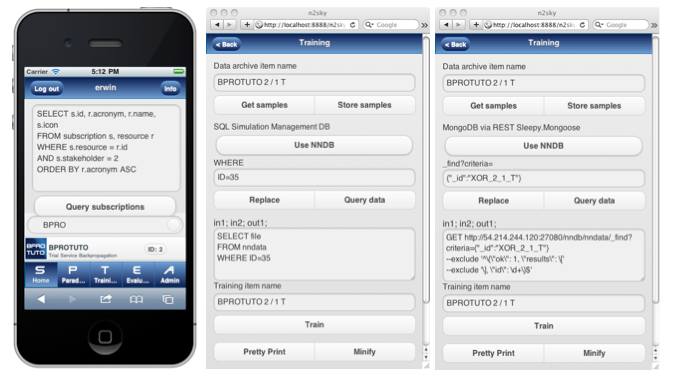
\includegraphics[width=\linewidth]{components/2/old_arch.png}
  \caption{Current N2Sky User Interface}
  \label{fig:old_arch}
\end{center}
\end{figure}


After signing in user getting subscription form, paradigm service and paradigm metadata views without any field description. Small titles unfortunately not always self-describing. Application in general oriented on the group of users, who are came from IT area. In some forms they can type queries, but the fields are not type safe and there is no autocomplete.
Representation of neural networks trained model is not readable. The model represented as a raw JSON or XML file, user can not download it. The last point is a design in general that does not look up-to-date and user attractive. 


\item[User interviews and Questionnaire.]
User insights are very important. It helps to understand a nature of the problem. But if user find something confusing, the interviewer need to dig deeper to stress the importance of particular insight. Unfortunately there were no analytics data and any reviews regarding UI and UX, so with a small group of colleges the current UI of N2Sky was reviewed. 
The following questions were derived (Q1-Q5): 


\begin{itemize}
\item Q1: "How N2Sky can help you with a developing of your neural network?"
\item Q2: "What was the most difficult part by creating a new model?"
\item Q3: "Did you face any problems during spawning your neural network? If yes, then what kind?"
\item Q4: "Did you find out something new, when other users were performing testing against your neural network?"
\item Q5: "What did you miss during using an N2Sky?"
\end{itemize}	

There were 5 students interviewed. All students were together in one group. Summarise answers (A1-A5) according to questions (Q1-Q5): 

\begin{itemize}
\item A1: N2Sky gives possibility to test the own neural network. Unfortunately, if the user does not have a neural network it is impossible to test the application.   
\item A2:  User face difficulties during creation of the new neural network model. User interface user technical jargon and it is not intuitively understandable.  
\item A3:  Spawning a neural network was pretty clear process, but it was not really clear if neural network ready to use or not.
\item A4:  Logging of the training data is very useful. The neural network owner can see how his network behaves with a different training and testing data.
\item A5:  User wants perform testing and training on already existing neural networks. 
\end{itemize}	


\item[Current application design mapping.]

After studying the answers it is possible to highlight weak parts of application. This approach will show a big picture of the current application design:

\begin{itemize}
\item Arbitrary user needs to know multiple technologies and programming languages just simply to reuse existing neural network. 
\item Too much information on every view. The purpose of view is overloaded. Each view has too much functionality, which makes user to loose a focus.
\item Application works relatively slow. Even if there some processes behind happening, the user des not know it.
\end{itemize}

Important is to face the problems, but does not "reinvent the wheel".  As \hl{Joel Spolsky the} founder of Netscape and CEO of Stack Overflow said, ??throwing away the whole program is a dangerous folly?. That is why it was decided to consider the problems of current N2Sky design and reuse working ideas in refactored system

\item[Application Maintenance.]
N2Sky was monolithic standalone application, which included all services in one and was deployed as a whole. The application was not distributed.  In case if one of the services doesn?t work correct, the whole application is not usable. 
Originally the previous version of N2Sky was written fully on Java. There were hundreds classes, providers and services in one project. Developer will spend hours to maintain this kind of project. To find an issue in a big application is always a challenge.  Small changes are causes a subsequence changes. If the software breaks after change, than it will additional high effort to fixed it. As Robert Cecil Martin wrote in his book ?Clean Code?: ?The code is hard to understand. Therefore, any change takes additional time to first reengineer the code and is more likely to result in defects due to not understanding the side effects? \hl{[https://www.amazon.com/Clean-Code-Handbook-Software-Craftsmanship/dp/0132350882]}.  He categorizes this kind of code into ?Smell? code. Unfortunately N2Sky from maintain perspective had all problems, which Mr. Martin

That is why N2Sky is shifted from monolithic system to container based system with an independent micro services which located on cloud environment. 
The frontend and frontend services are lightweight and easy to maintain parts of the big application. If something goes wrong, the developer knows exactly where is the problem. It is close to impossible to break something else during fixing because of independence of services. 
Additionally there are monitoring and alerting systems which are supporting developers during maintenance.  Early it was not possible to say if application works correctly or even it still running. Users could get a bad experience while they using an application in case if it does not work correctly. But now it is possible not only notify an application administrator about some problems, but also to predict potential threads. 
\end{description}


\subsubsection{Refactoring the User Interface}\label{Refactoring the User Interface}

User Interface (UI), an abbreviation of user interface, allows the interaction of a user with a program through graphical visualization made by text, icons, buttons and pictures. While deciding the design of a user interface there are some highly recommended features also known as heuristics, which was invented by hl{Jakob Nielsen}. It was decided to apply the following 10 general principals of interaction design to N2Sky:

\begin{description}
\item[Simple and natural dialogue.]  N2Sky will have an simple UI which is understandable for any user, even if the user is not an expert. Every icon and every navigation or action button will be self-describing. The application will follow the slogan ?less is more?. No more overloaded views. The idea of N2Sky UI design is that one particular view is responsible for one particular function or group of functions which a coupled tight together.
\item[Speak the users language.] Developing N2Sky was concentrated on user perspective. There is no technical jargon for arbitrary user.
\item[Minimize user memory load.] There is no multiple options, functions or menus on one view. There is also no multiple ways to do the same thing. N2Sky teach user how to make things done with a one existing and convenient workflow. 
\item[Consistency.] N2Sky has similar layouts, fonts, colors, icons types structures and organization throw entire application. The user should get the same visual experience on every view.
\item[Feedback.] Every action, process or even error will be notified. User will know exactly what is happening with a system with clear and understandable messages.
\item[Clearly marked exits.]  Every push to action button has short and clear caption.
\item[Shortcuts.] N2Sky has multiple user types. One of the types is the expert users, which are advanced user in neural network and artificial intelligence topics. For this kind of user is provided more technical jargon, but this UI is separated with an arbitrary users.  
\item[Good error messages.] Every notification is clear inclusive an error massage if occurs. Every message has a prices and simple description.
\item[Prevent errors.] In N2Sky implemented logical structure of UI components. There are constrains which are helps user in workflow. For example user will always get a default value of any input.
\item[Help and documentation.] N2Sky will have tutorials that describe the user workflow. The expert users will also get a API documentation with a detailed description and sample requests. 

\end{description}

Each and every one of these heuristics is connected to a crucial idea that is usability. By mentioning this idea, a straightforward relation with the UX follows since this is also one of the key concept that grows along the rapid development of technology. UX is known as user experience and it describes the perspective and feelings a user gets when interacting with product. It deepens into such aspect as the users inner circumstances and the nature of the created design. The goal is to achieve such a system that offers distinguished user experience and accomplishes the most of aspects. As above mentioned, usability.  \hl{(1)}
Putting both of UI and UX in a comparison, to all appearances the user interface is the target on the appearance and functionality of the product and its tangible details.  Furthermore, the user experience is the general experience that the user manages throughout the whole use.   \hl{(2)}
UI will concentrate on the appearance and design of the product, rather than the functionality. The intent of it relies in the visual design and layout. UI covers issues such as how a button is supposed to look like, how the errors are going to appear or is it visually comprehensible meaning which colors or font type shall be used for a better perceptibility of the product.  \hl{(6)}
UX points its focus on the involvement of the user while interacting. It is measured by a variety of tests and researches done to achieve a higher satisfaction on the users side.  \hl{(4)}
Though their differences, the only matter which relates both UI and UX is their priority, in other words, the user. When expanding the concept of both these definitions it can be concluded that one co-exists with the other. There would not be user interface without user experience and vice versa. 

 \hl{TODO // CHECK MERSI DOKU}

\subsubsection{Introducing a new User Experience Design}\label{Introducing a new User Experience Design}

 \hl{TODO}


\subsection{Contemporary N2Sky Architecture}\label{Contemporary N2Sky Architecture}

The user-centered design is a fundamental requirement for N2Sky. Looking back on past experiences with the application, there were identified the real capabilities and needs of a users. N2Sky was moved from a complex monolithic system to an easy understandable application. Every interested user without having a deep knowledge in the neural network field can freely use N2Sky.  The goal was to save and gain the current functionality of the application and decrease the visual complexity of it. 

\subsubsection{Architecture design}

N2Sky is a simulation platform, which allows all involved stockholders to use it for computational purposes. In order to achieve high performance and scalability, it was decided to use the microservices architecture. This approach is used not only on backend services, but also with frontend and its services. 

\begin{figure}[htbp]
\begin{center}
  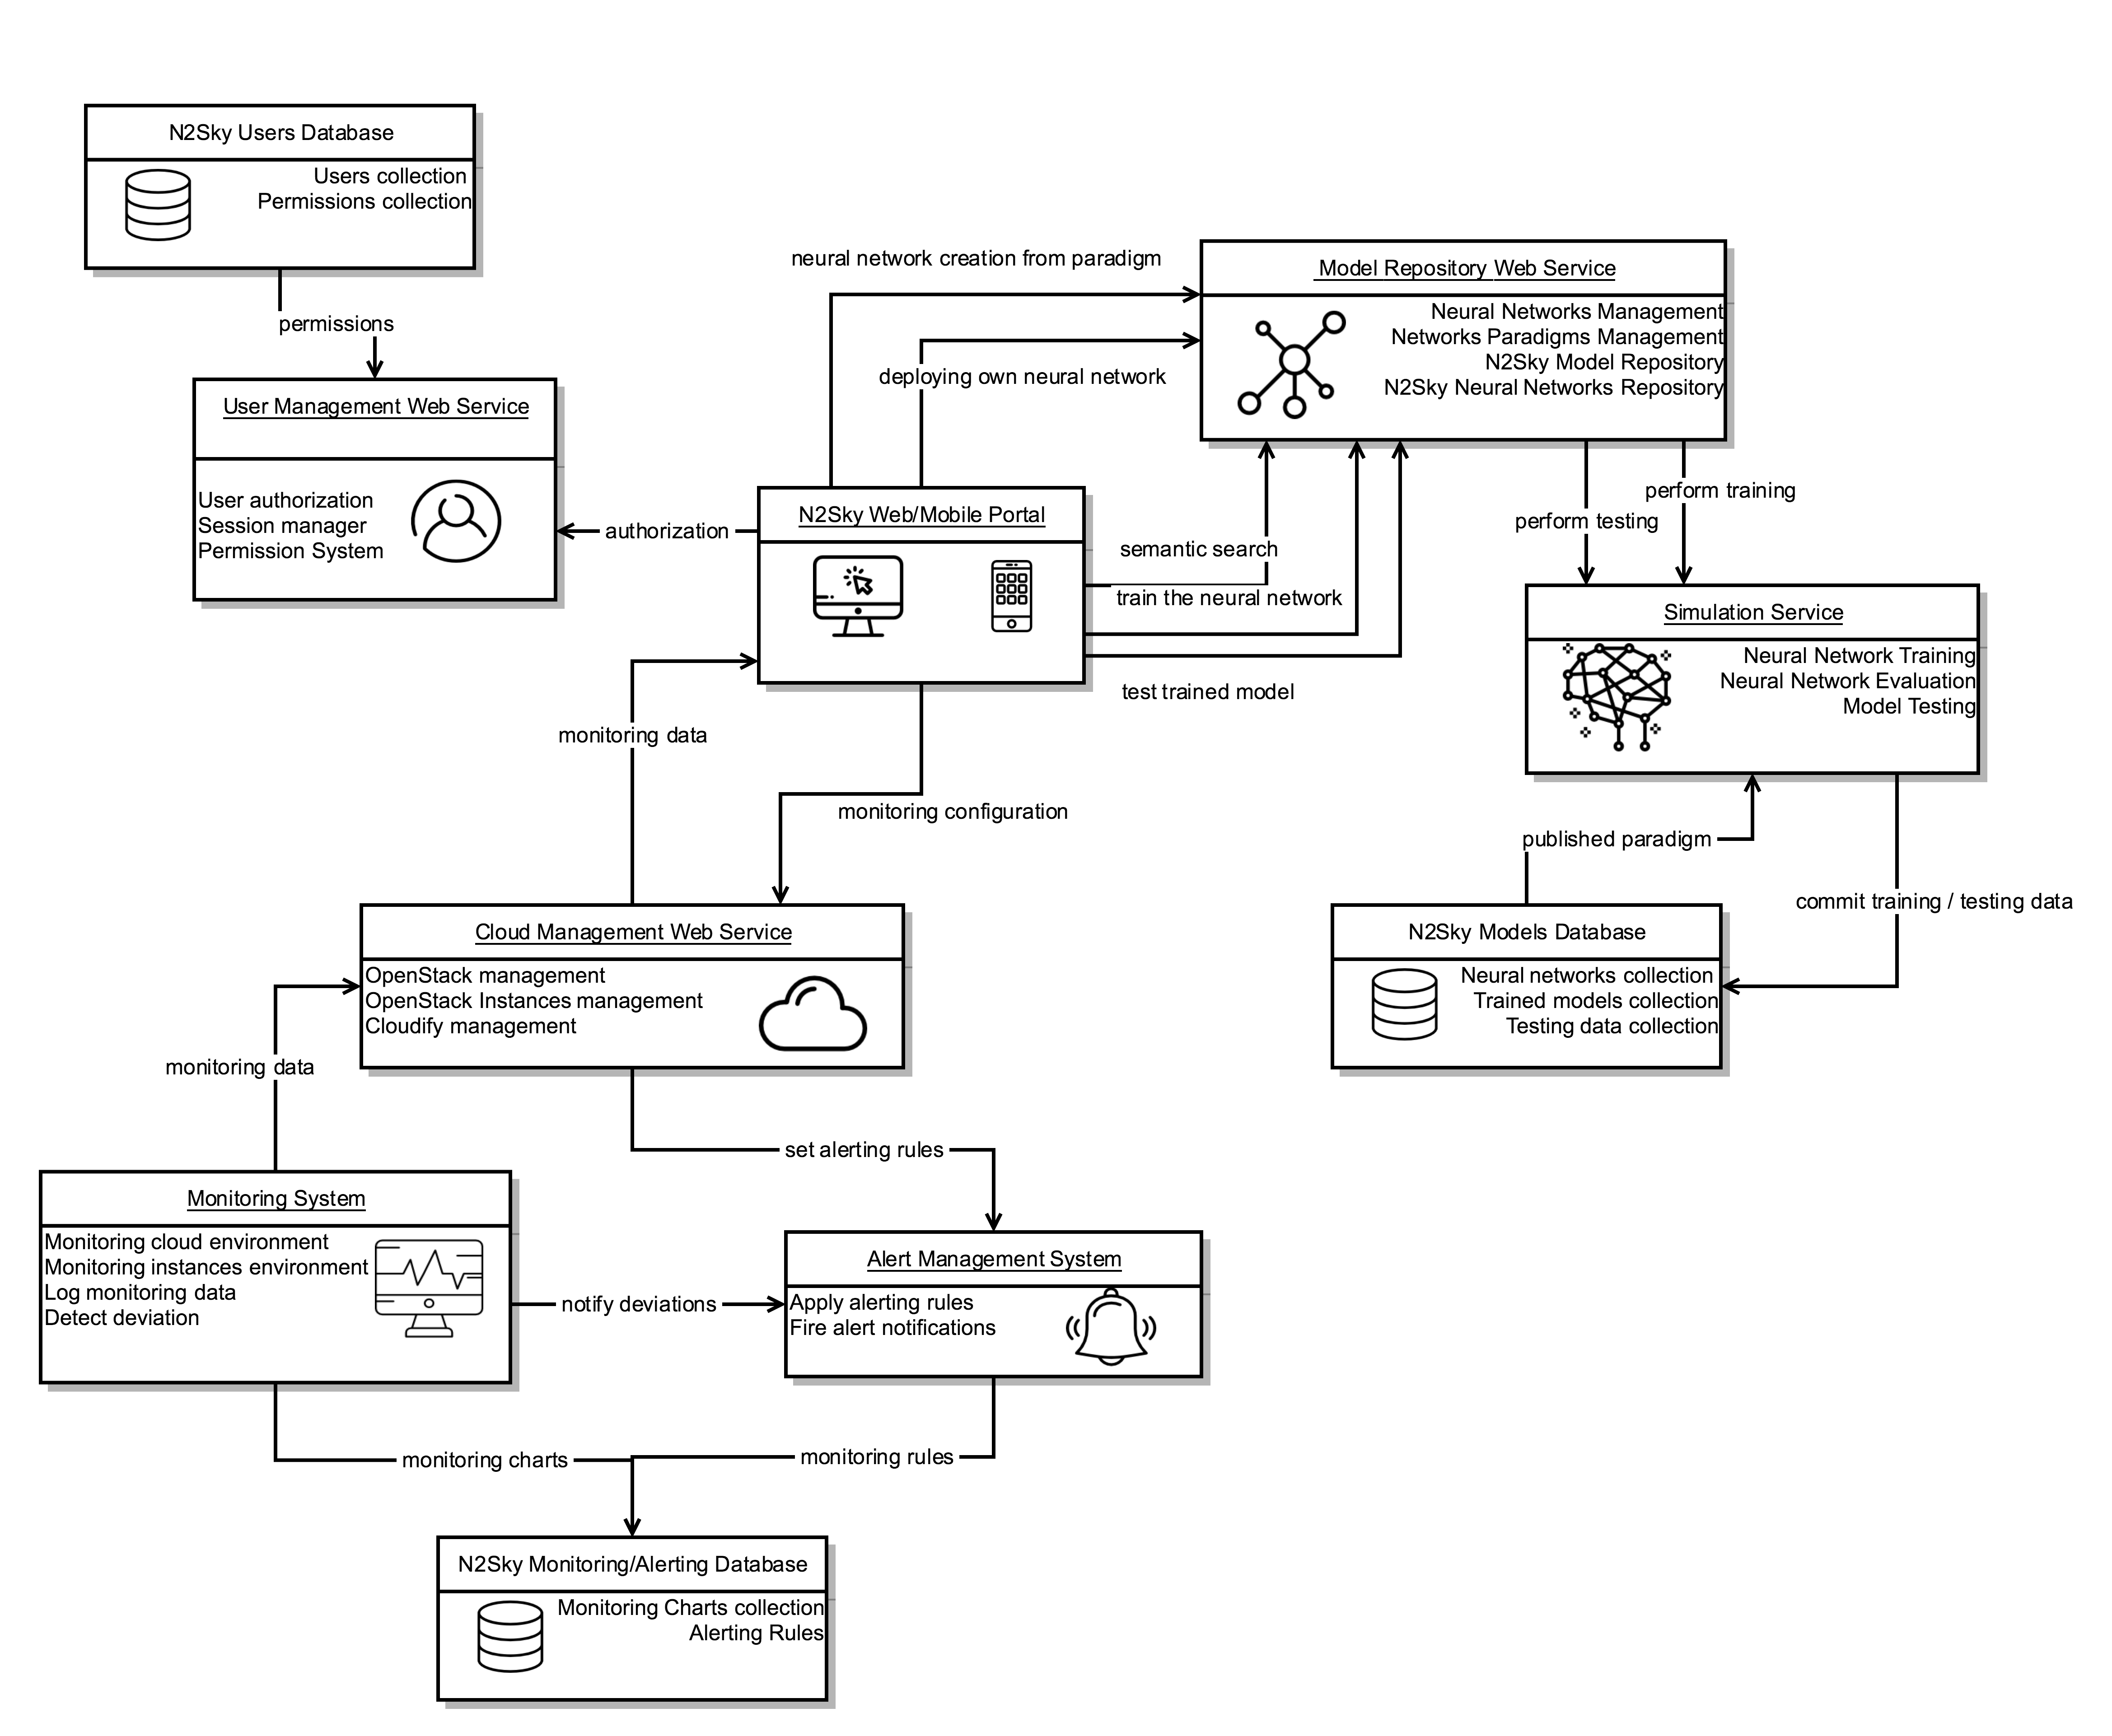
\includegraphics[width=\linewidth]{components/2/new_arch.png}
  \caption{Contemporary N2Sky architecture overview}
  \label{fig:newarch}
\end{center}
\end{figure}

The architecture overview, which shown in ``Fig.~\ref{fig:newarch}'' represents microservices architecture. 

The centred figure is the N2Sky Web/Mobile portal. Is is frontend application of the N2Sky, which consist of modular subsystems. Since the frontend application has responsive design it supports desktop devices as well as mobile devices. 
To support Software as a Service distribution every web service can work independently. It means that the stackholders can use N2Sky via web portal as well as use N2Sky API.
N2Sky API allows  stackholders:

\begin{itemize}
\item Authorise in the System
\item Create new neural from existing paradigm
\item Deploy own neural network on N2Sky environment 
\item Perform training against own as well published neural network
\item Perform testing against trained models
\end{itemize}

Almost everything is available for arbitrary stackholder, except cloud services. In order to cloud service as a service, the user has to install it on his own cloud environment. This approach supports Platform as a Service distribution. Cloud services only for system administrator and for granted users are available. 


\subsubsection{N2Sky Services}\label{N2Sky Services}

 N2Sky implements microservices architecture. It has 3 main web services as it shown in ``Fig.~\ref{fig:newarch}'' :
 
\begin{itemize}
\item User Management Web Service
\item Model Repository Web Service
\item Cloud management Web Service
\end{itemize}

Every web service use other services which are not exposed to the public. It was made in order to support application encapsulation. Encapsulation of web application helps to prevent security issue. One of the crucial crucial process in N2Sky is the neural network training. This process takes almost all resources of the environment, that is why it is not exposed. Such a processes can be triggered only by web service, which can be blocked if environment is overloaded.

Consider the following web services in details and which processes and services they are encupsulate:  

\begin{description}
\item[User Management Web Service.]   This web service responsible for permissions and user management and it has its own database. User can authorise in the system and get a session token. Every token is an unique collection of numbers and latin letters. Token is assign to the authorised user and will be save until user is active. If user is not active in the next 3 hours, the session token will disappear. If user still have an active browser session, the authorisation token will be revalidate. If user trying to make some illegal request or behave too active, the authorisation token will be revoked and the system administrator will be notified about this incident. 

Every user encapsulate permission level. There two different types of permissions:
\begin{itemize}
\item Administrator permission. It means, that the user has full granted permission throw entire application.
\item Regular permission. The user has access only for his own as well as public available resources.  
\end{itemize}
\item[Model Repository Web Service.]  Model Repository Web Service is the core service of N2Sky. Authorised user can create a new project, add there neural network from chose paradigm or deploy own one. Every newly created project is assign for one user and can not be shared, only system administrator can look up into other users projects. This functionality also limited by User Management Web Service. 

Using this service user can create a neural network from proposed paradigms as well as upload his own neural network in \hl{ViNNSL} format. This functionality exposed via service so that every user can use it either from N2Sky web portal or via HTTP request directly on web service.

There are two services embedded to the Model Repository web service and not exposed:

\begin{description}
\item[Training service.]  This service provides neural network training functionality. It is not possible to perform training to make direct request on service endpoint. 

In order  to perform training the user has to know training input parameters and type of training file which ca be accepted. This information is stored in ViNNSL schema. 
 
Only Model Repository web service can trigger this service after being insured that environment available and ready to perform tests. Training a is long term process, but it does not block an entire application. This service write log data to the instance. Model Repository repository makes a callback to training service in order to check if training is completed. If training still processing, the Model Repository Service will fetch the log data in order to present current training result. User can also decide to stop training process if he is satisfied with the current result.

If user perform training on his own neural network he can also log result about his network and enviroment behaviour. 
\item[Testing service.] The testing service allows users to evaluate a trained model.  Testing data is described in ViNNSL format. Normally testing is not a long term process, because it is running agains trained neural network model. Since there is absolute freedom by neural network structure customisation, the testing process can be inefficient and could take some resources from the environment. Considering this face it was decided to encapsulate this process too. 
\end{description}

 \item[Cloud management Web Service.]  Cloud web service is originally available only for system administrator. This service can manage OpenStack environment and Cloudify container management system. On every OpenStack instance as we as on OpenStack itself the monitoring management system service is installed. Every monitoring management system has its own metrics configurations and alerting rules. The monitoring service is only exposed via Cloud management web service. 
 
 Cloud management service supports Platform as a Service distribution. The system administrator can configure the service according to his needs. All rules, including configuration rules for monitoring and alert management systems, can be adjusted on demand.  


\end{description}



 
 
\subsubsection{Modular frontend application design}
The central concept of the application is to support the \hl{Software as a Service (SaaS)} and Platform as a Service (PaaS) distributions.  N2Sky consist of two modules: administration module, main application module as it shown in ``Fig.~\ref{fig:modular_design}''.

\begin{figure}[htbp]
\begin{center}
  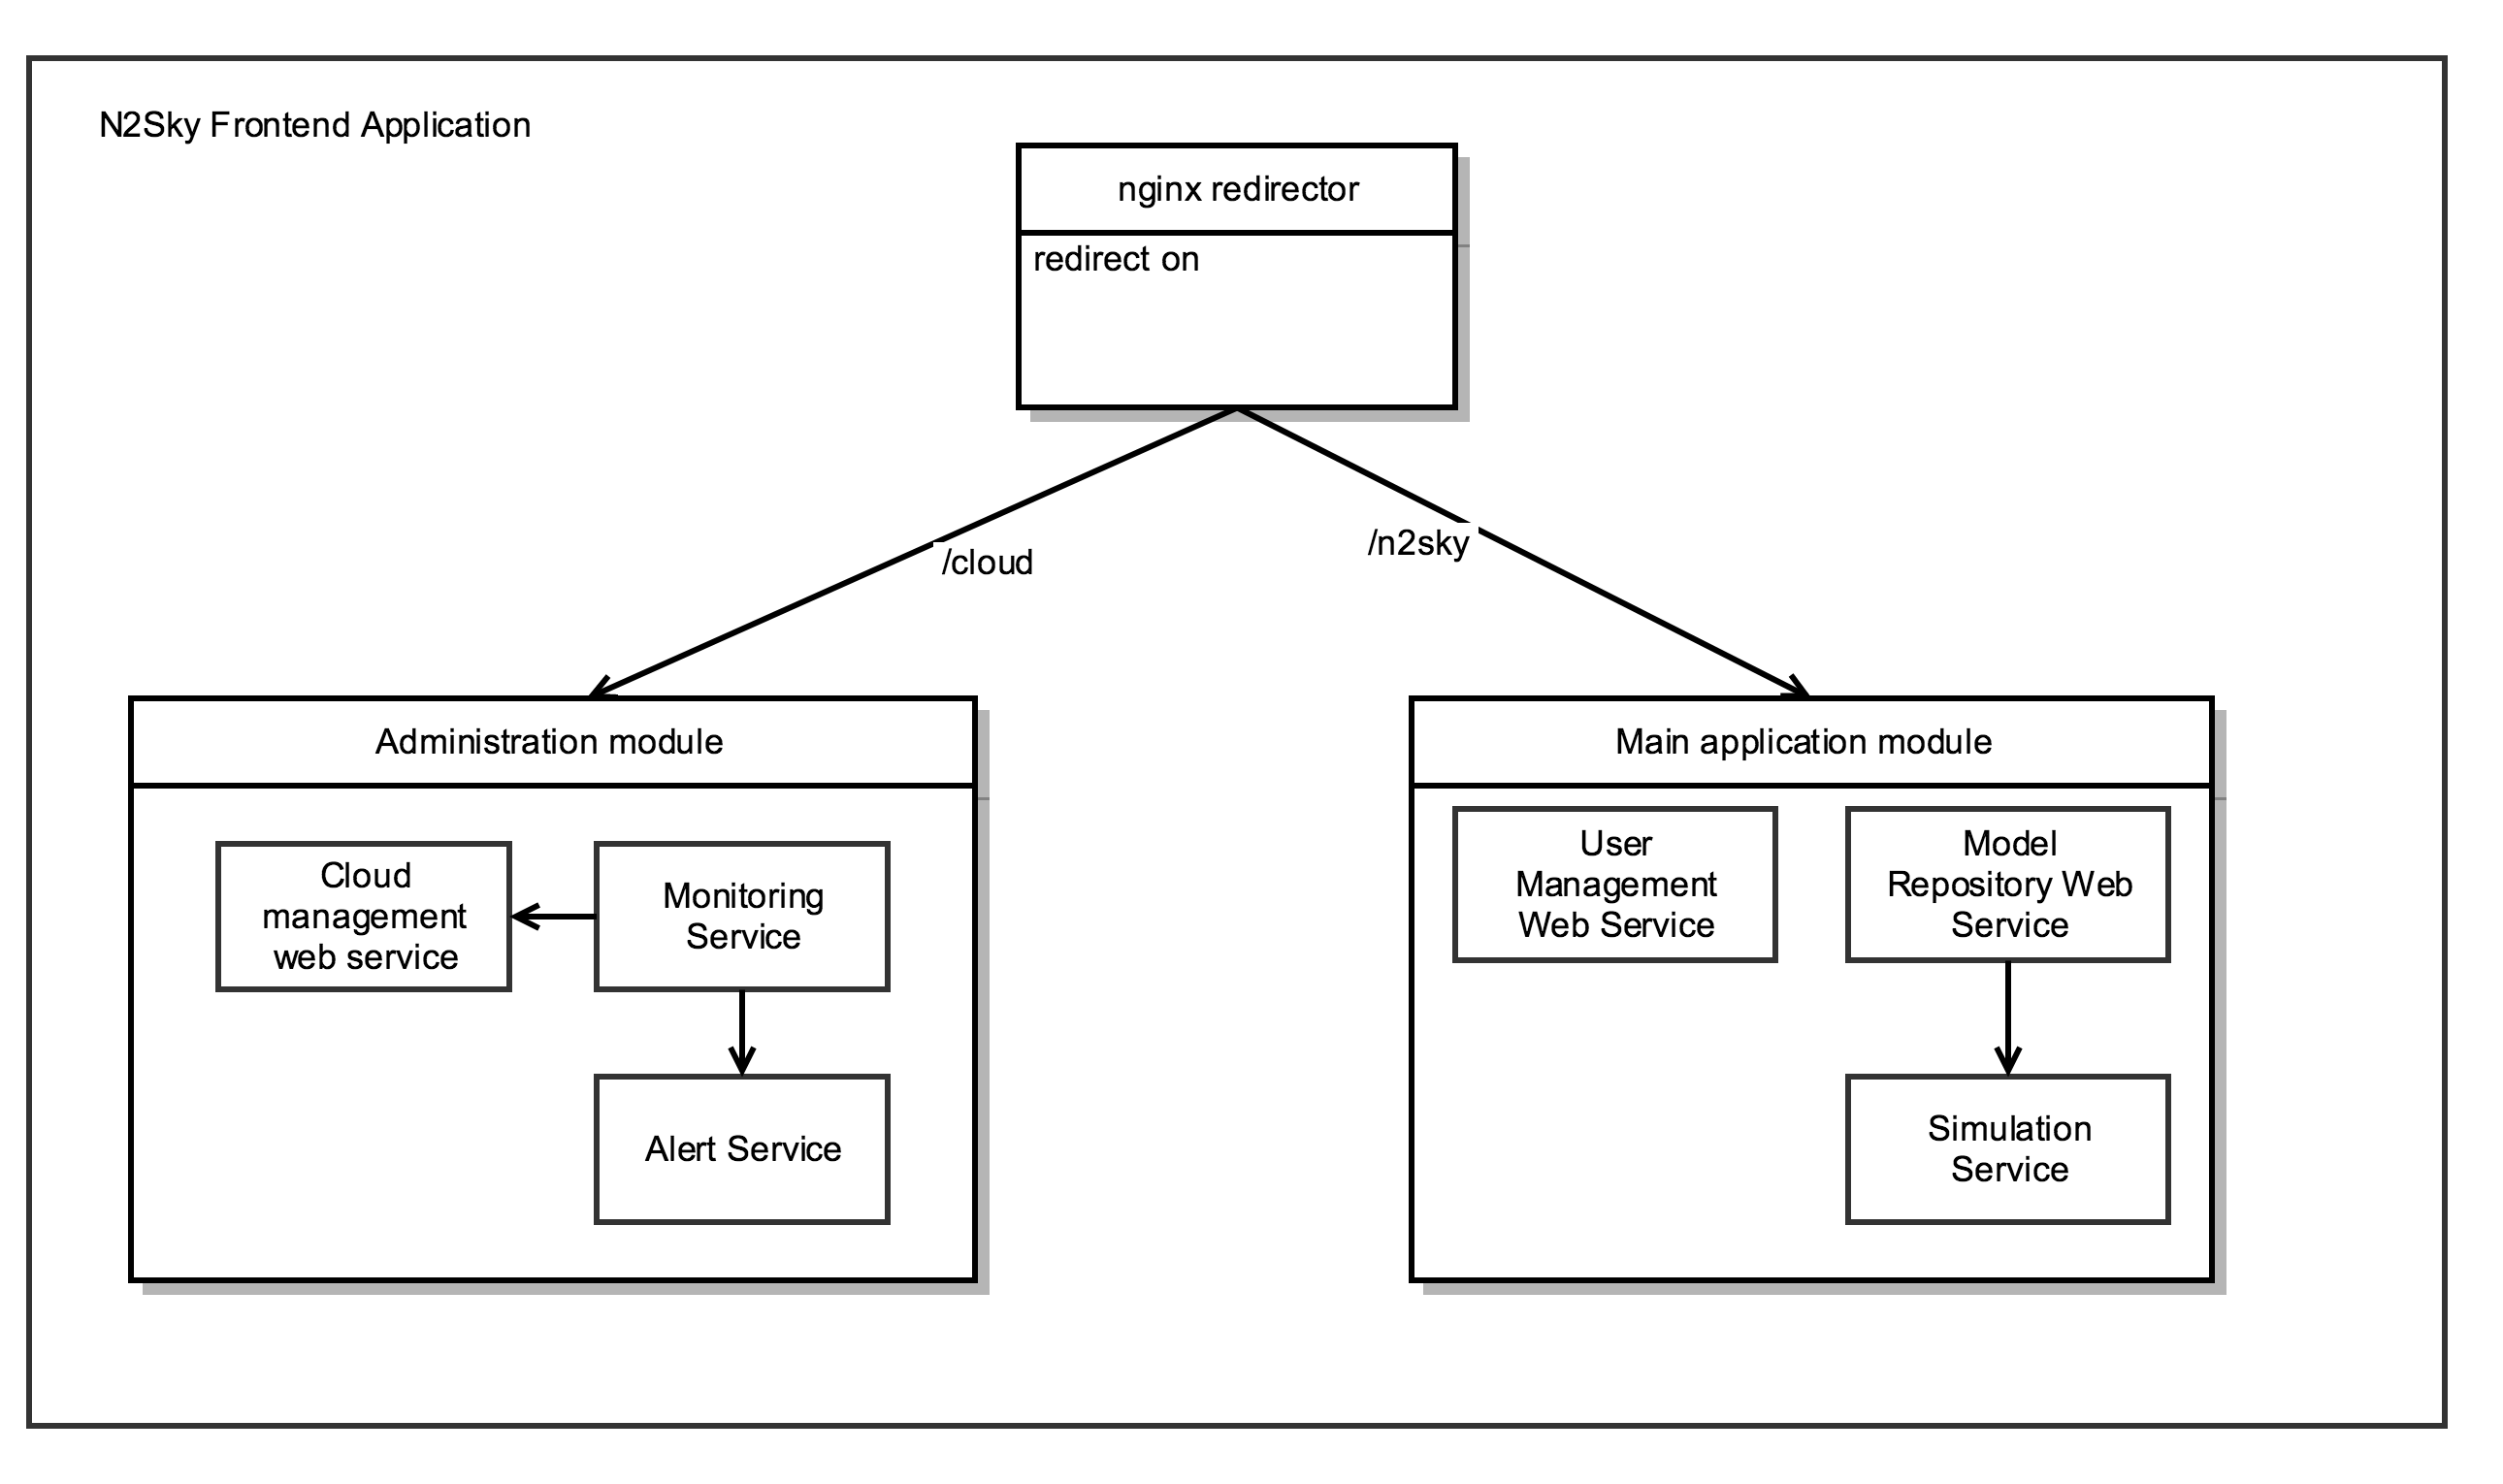
\includegraphics[width=\linewidth]{components/2/modular_design.png}
  \caption{N2Sky frontend application and its services}
  \label{fig:modular_design}
\end{center}
\end{figure}

\begin{description}
\item[Redirector.] When the user goes to N2Sky web portal, first he will be dealing with a redirector. The redirector is a small service, which is build on Nginix server. The purpose of it is to redirect the user depending on URL path.
\begin{description}
\item[/cloud] redirects to "Administration module"
\item[/n2sky] redirects to "Main application module"
\end{description}


\item[Administration module] The administration module allows the system administrator to control the environment. The module supports OpenStack and Cloudify monitoring. Managing is possible through the application dashboard. It also contains custom monitoring and an alerting management system, which can be installed on any server within the N2Sky user interface. The administration module implements PaaS. It is fully configurable and wrapped into the open source project in order to make the module accessible to the third-party applications. 
\item[Main application module] The main application module is the central module of N2Sky. Within this module, users can use, train and test existing neural networks. It is possible to reuse the neural network paradigms and create own neural network. N2Sky allows to deploy own network and store data in cloud. Module services are supporting the SaaS distribution. Experts can use an application directly through the N2Sky API or they can integrate N2Sky services to their own application. 
\end{description}


 

\subsubsection{Technology Stack}\label{Technology Stack}

N2Sky today is the cross-platform handy application with a responsive design. Create own framework from scratch would be time consuming. To build cross-platform framework just for N2Sky is an absurd. After some research of most popular and common used frontend frameworks following candidates were listed: 

\begin{description}
\item[Vaadin.] Java framework, which compiles Java code into JavaScript components. Vaadin supports cross-platform application, but not fully. It is possible to wrap an applicaiton into container and deploy it only as an android application.

\begin{description}
\item[Benefits.] Easy to develop in Java. Developer does not have to think about JavaScript functionality. There are dozen of predefined components like: buttons, input fields, frames etc. Customisation is also possible. 
\item[Obstructions.] Deployment process is a blockage process. There is no "hot redeployment" available. Even if developer win some time by build components in Java, he will lose much more time by continuous redeployment. 

Java application need some server which supports JVM, it means that server should have much more memory then some other frameworks, which are written on JavaScript language.  
\end{description}

\item[ReactJS.]  JavaScript framework, which supports JSX programming language. 
\begin{description} 
\item[Benefits.] The main idea is to write HTML code in JavaScript. ReactJS supports hot redeployment.  React-Native extension for this framework, which allows to wrap the whole application mobile as well as desktop application.
\item[Obstructions.]  Difficult to support a big project. JSX is not a type safe programming language. Exception handling also need to be done by developer.  
\end{description}
\item[AngularJS.] JavaScript framework, which supports TypeScript programming language.
\begin{description} 
\item[Benefits.] The main idea is to write JavaScript code in HTML.  AngularJS same as ReactJS supports hot redeployment.  It does not have native support for all mobile devices, but is possible to wrap it using IONIC framework. 
\item[Obstructions.]  AngularJS compiles TypeScript code into JavaScript core and sometimes compilation fails because TypeScript is a new language and it is not fully adopted for browsers. 
\end{description}
\end{description}
 
 Vaadin does not fit N2Sky needs, but AngularJS and ReactJS could fit perfectly. Both of this frameworks are written on JavaScript and have big corporations behind: AngularJS was developed by Google and ReactJS was developed by Facebook. Since N2Sky has to support fully cross-platform architecture it was decided to choose ReactJS. With this framework N2Sky has a potential to be multi-platform application in the future. 
 

Furthermore, backend has microservices architecture to support scalability. After choosing JavaScript framework for frontend it will make sense to user JavaScript in a backend too, so that server would be small and fast. Each one of the microservices is developed on NodeJS Framework server, which implies efficiency and lightweight. 

N2Sky is a cloud-based system. OpenStack cloud platform supports this approach. Since N2Sky user OpenStack API for administration dashboard, the original OpenStack dashboard was no more needed. Every backend and frontend service is deployed on OpenStack instance. Every instance is absolutely scalable, which allows to find a best enviroment for every service. 

Every OpenStack instance is a server with either Debian or Ubuntu operational system. Every instance as well as OpenStack itself has to be monitored 24/7, that is why there was Monitoring Management System developed. The basis of this system is Prometheus monitoring system, which gives full access to all information of any server were its was installed. Prometheus has an open API, which is used by N2Sky. Using Prometheus there were charts and graphs developed and integrated into N2Sky. Alert Management System, which is a part of N2Sky, is also using  Prometheus API in order to detect deviation and notify on event occurred.

As a database it was decided to choose NoSQL one. There were two NoSQL databases under consideration ElasticSearch and MongoDB. 
ElasticSearch supports indexes. It is possible to configure index so, that is impossible to insert something which is not mapped by the index.  MongoDB does not user index approach, but MongoDB client supports schema. It was decided to use MongoDB schema and mapped ViNNSL schema to it in order to make it more understandable for other developers. 

For continuous delivery and quick configuration it was decided to use Jenkins Continuous Integration system. In case if the while system will go down it is possible to restore every service with a Jenkins Profiles.



\section{N2Sky Components}\label{N2Sky Components}

In the concept of N2Sky lies minimalistic and modern design. Dimmed tones of the UI components are used to make end-user to feel like he is using the professional expert system. Every component and element was carefully thought out in order to keep the same atmosphere throw the whole application. 

\subsection{N2Sky Frontend Application}\label{N2Sky Frontend Application}


Familiar elements and components help users easier navigate through the application. It is important to have common components and elements and do not mix up altogether. Every component and every GUI element should have the self-describing purpose. Building user interface components and elements are pretty same as developing some UML diagram. It is possible to group common parts and maximize reusability \cite{mod_ui_book}. 

It is important to consider the multiple end-users, devices, platforms as well as environments will be used. Throw heterogeneous context only needed elements has to be displayed. It is necessary to make view prototypes to determine if the particular component comfortable and easy to use \cite{Martinez2017}. 

\subsubsection{N2Sky Layouts Design}\label{N2Sky Layouts Design}


Design of N2Sky layouts was concentrated on principles of User interface design which were described in \cite{gui_layout}: 

\begin{description}
\item[Organise.]  All UI elements and components have to be ordered and not be chaotic. Randomise position or logically not understandable can confuse the user. 
\item[Consistency.] There are few types of consistency:
\begin{itemize}
\item Internal consistency, when elements are represented in the same place in the familiar components. 
\item External consistency, when few elements are looking a little bit different, but the same functionality. This happens often on different devices, especially on mobile devices.
\item Real-world consistency, which brings real-world symbols into application UI elements.
\end{itemize}
\item[Screen Layout.] There are few screen layouts: 
\begin{itemize}
\item Grid layout, which organizes all components into blocks, like menus, navigation bars etc. 
\item Standardise the screen layout, which mostly used on screens with restrictions.
\item Group related elements, which is usable for smaller screens.
\end{itemize}

In N2Sky Grid, the layout is used since it is possible easily to apply responsive design and reorganize grit items. 

\item[Navigability.] Navigation has to be always on user focus or at least easier to find how where and how to use navigation elements.
\item[Economize.] Following rules has to be applied: 
\begin{itemize}
\item Simplicity
\item Clarity
\item Distinctiveness
\item Emphasis
\end{itemize}
\item[Communicate]. The layout has to apply accuracy, typography, symbolism, multiple views to helps the user to communicate with the application.
\end{description}

\subsubsection{N2Sky Fundamental Layout}\label{N2Sky Fundamental Layout}

N2Sky Fundamental Layout is representing basic styling of the N2Sky application as is shown in figure \ref{fig:layout_basic}. 

\begin{figure}[H]
\begin{center}
  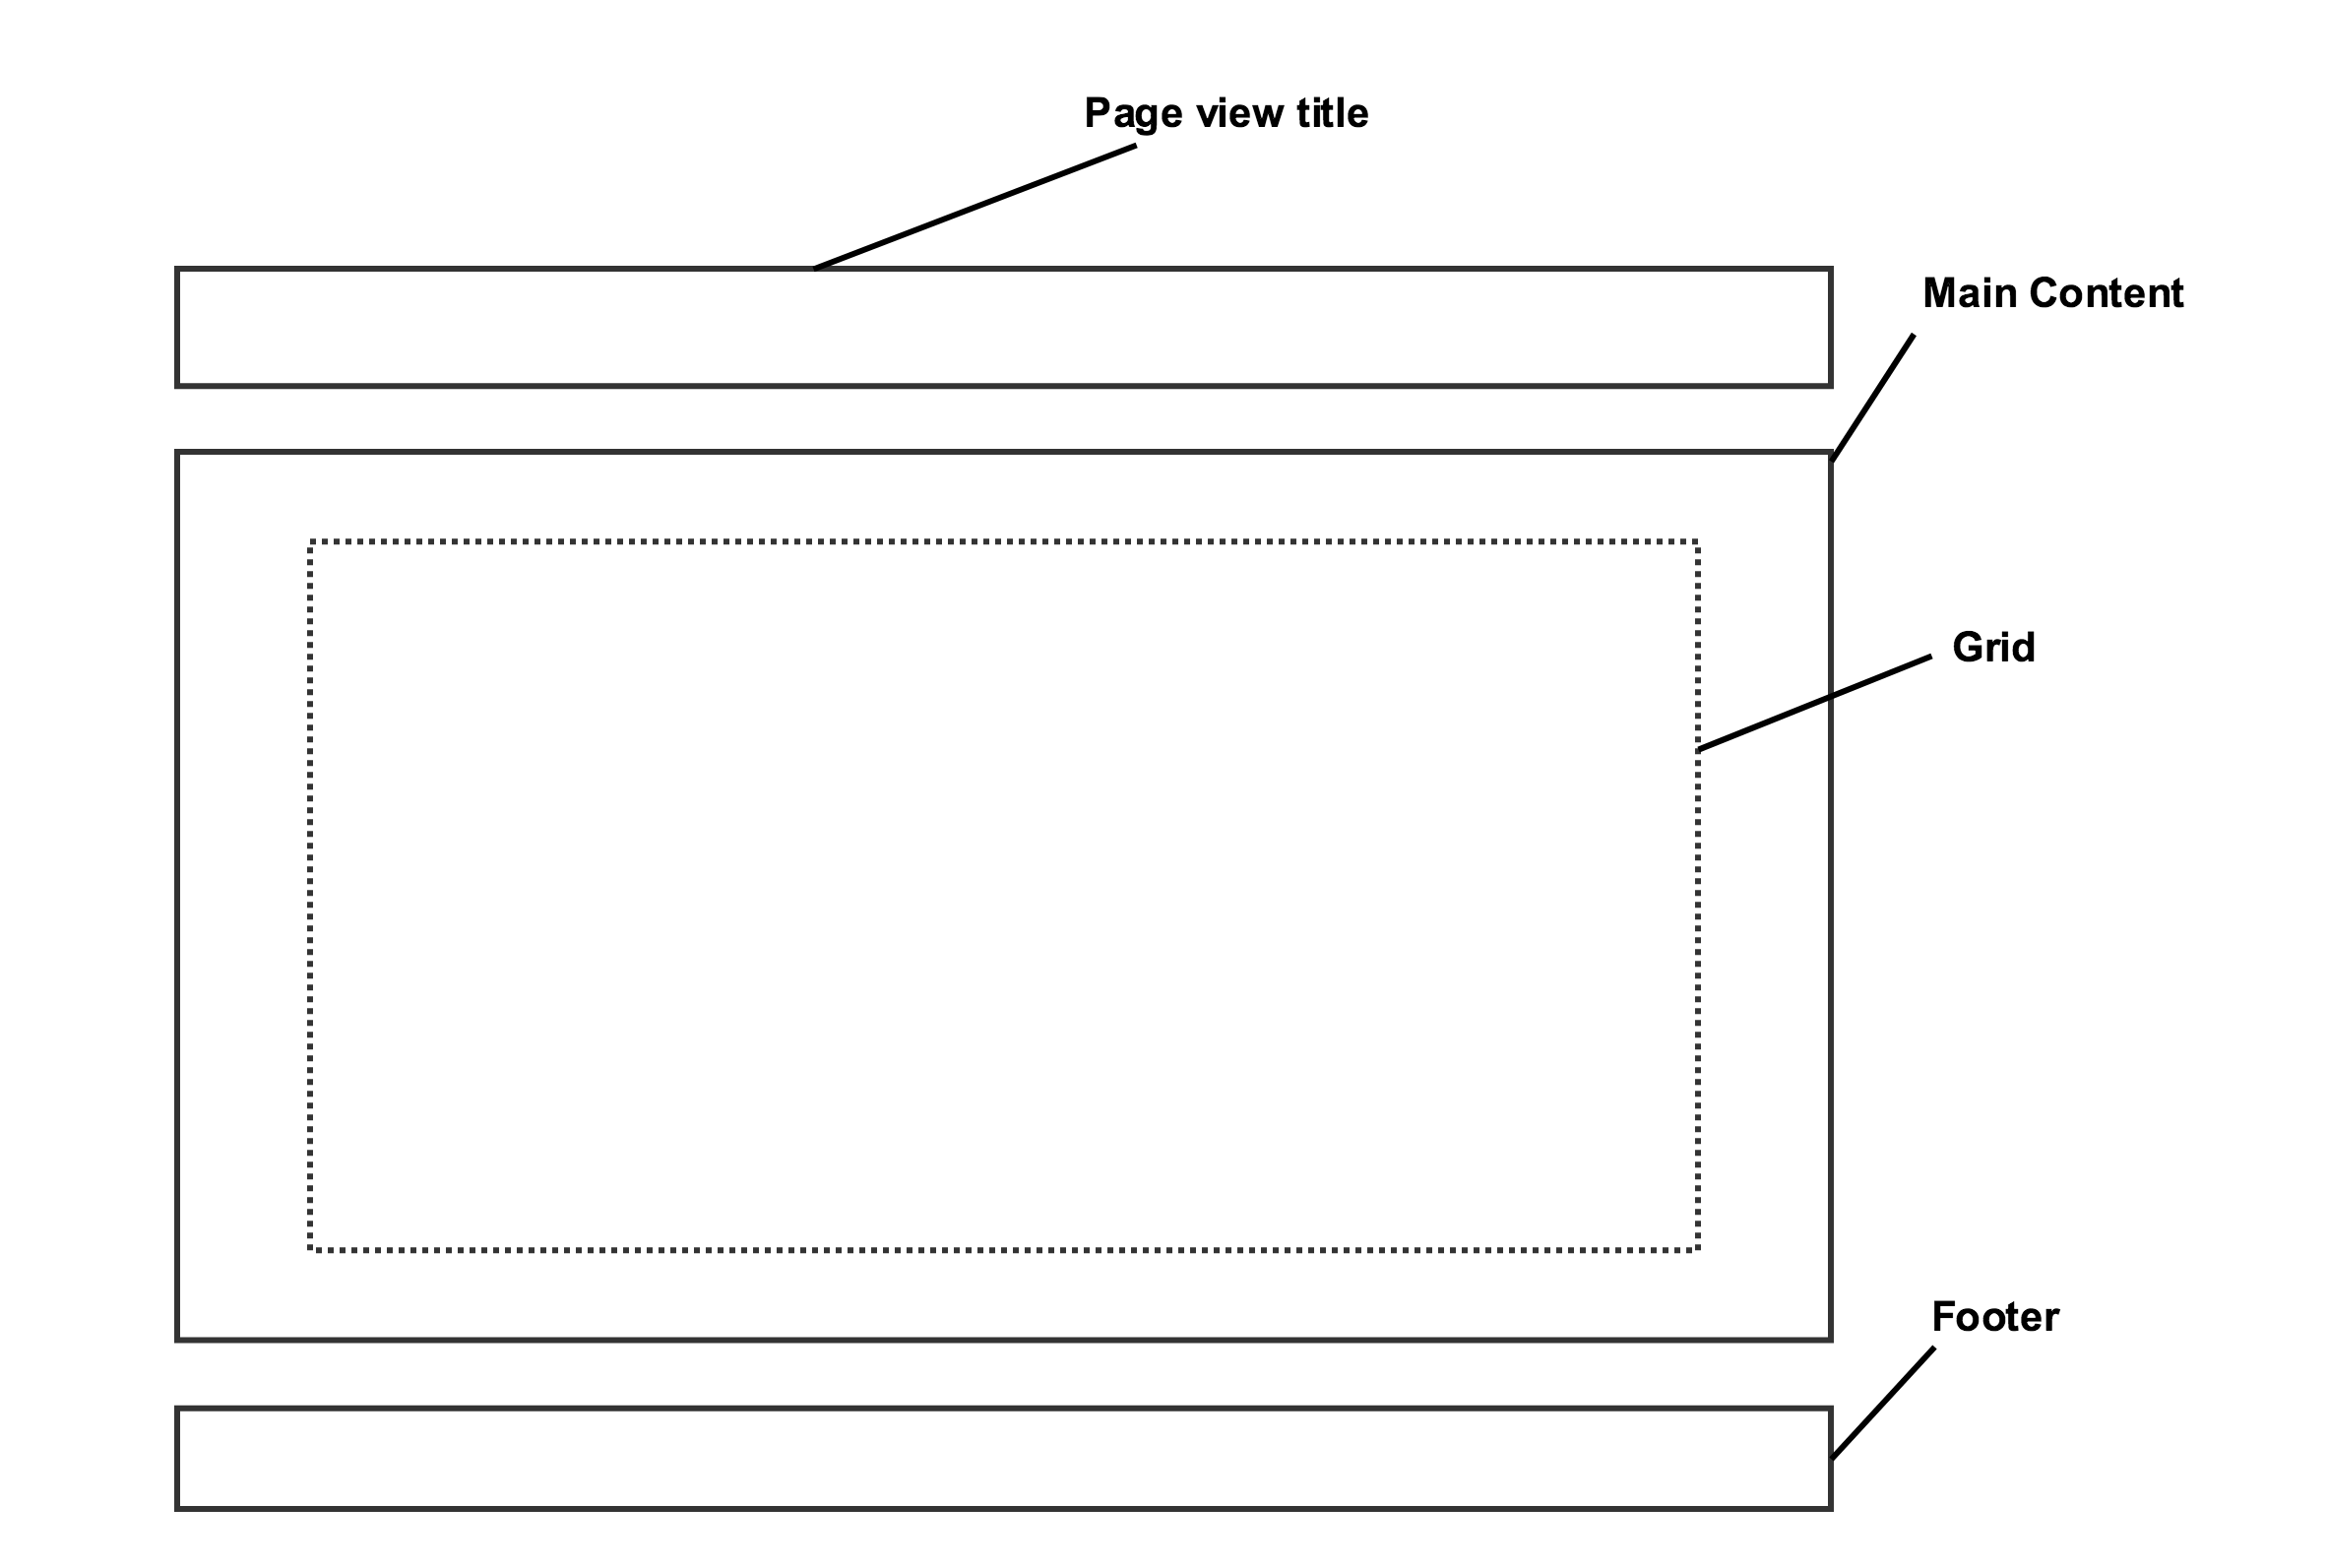
\includegraphics[width=\linewidth]{components/3/components/layout_basic.png}
  \caption{N2Sky Fundamental Layout}
  \label{fig:layout_basic}
\end{center}
\end{figure}

This layout applies styling like:
\begin{itemize}
\item Colors
\item Formatting
\item  Fonts
\item Positioning of elements and components
\end{itemize}



Fundamental Layout is a base layout which contains following elements:
\begin{itemize}
\item Page view title is a component with a caption and optionally an icon or push-to-action button
\item Main Content is centered component, which represent primary context. This component is always in focus of user and can contain one or more grid components.
\item Grid in basic layout represents positioning of elements, which can be displayed inside it. In basic layout in grid component is possible to add any elements. 
\item Footer is a component which goes across the whole application with a static data. Normally it is contacts and terms and conditions. 
\end{itemize}


\subsubsection{N2Sky Main Layout}\label{N2Sky Main Layout}

N2Sky Main Layout, which is shown in ``Fig.~\ref{fig:layout_main}'',  is extending N2Sky Fundamental Layout. Any changes in the basic layout will be automatically reflected in the main layout. Following components were added:

\begin{figure}[H]
\begin{center}
  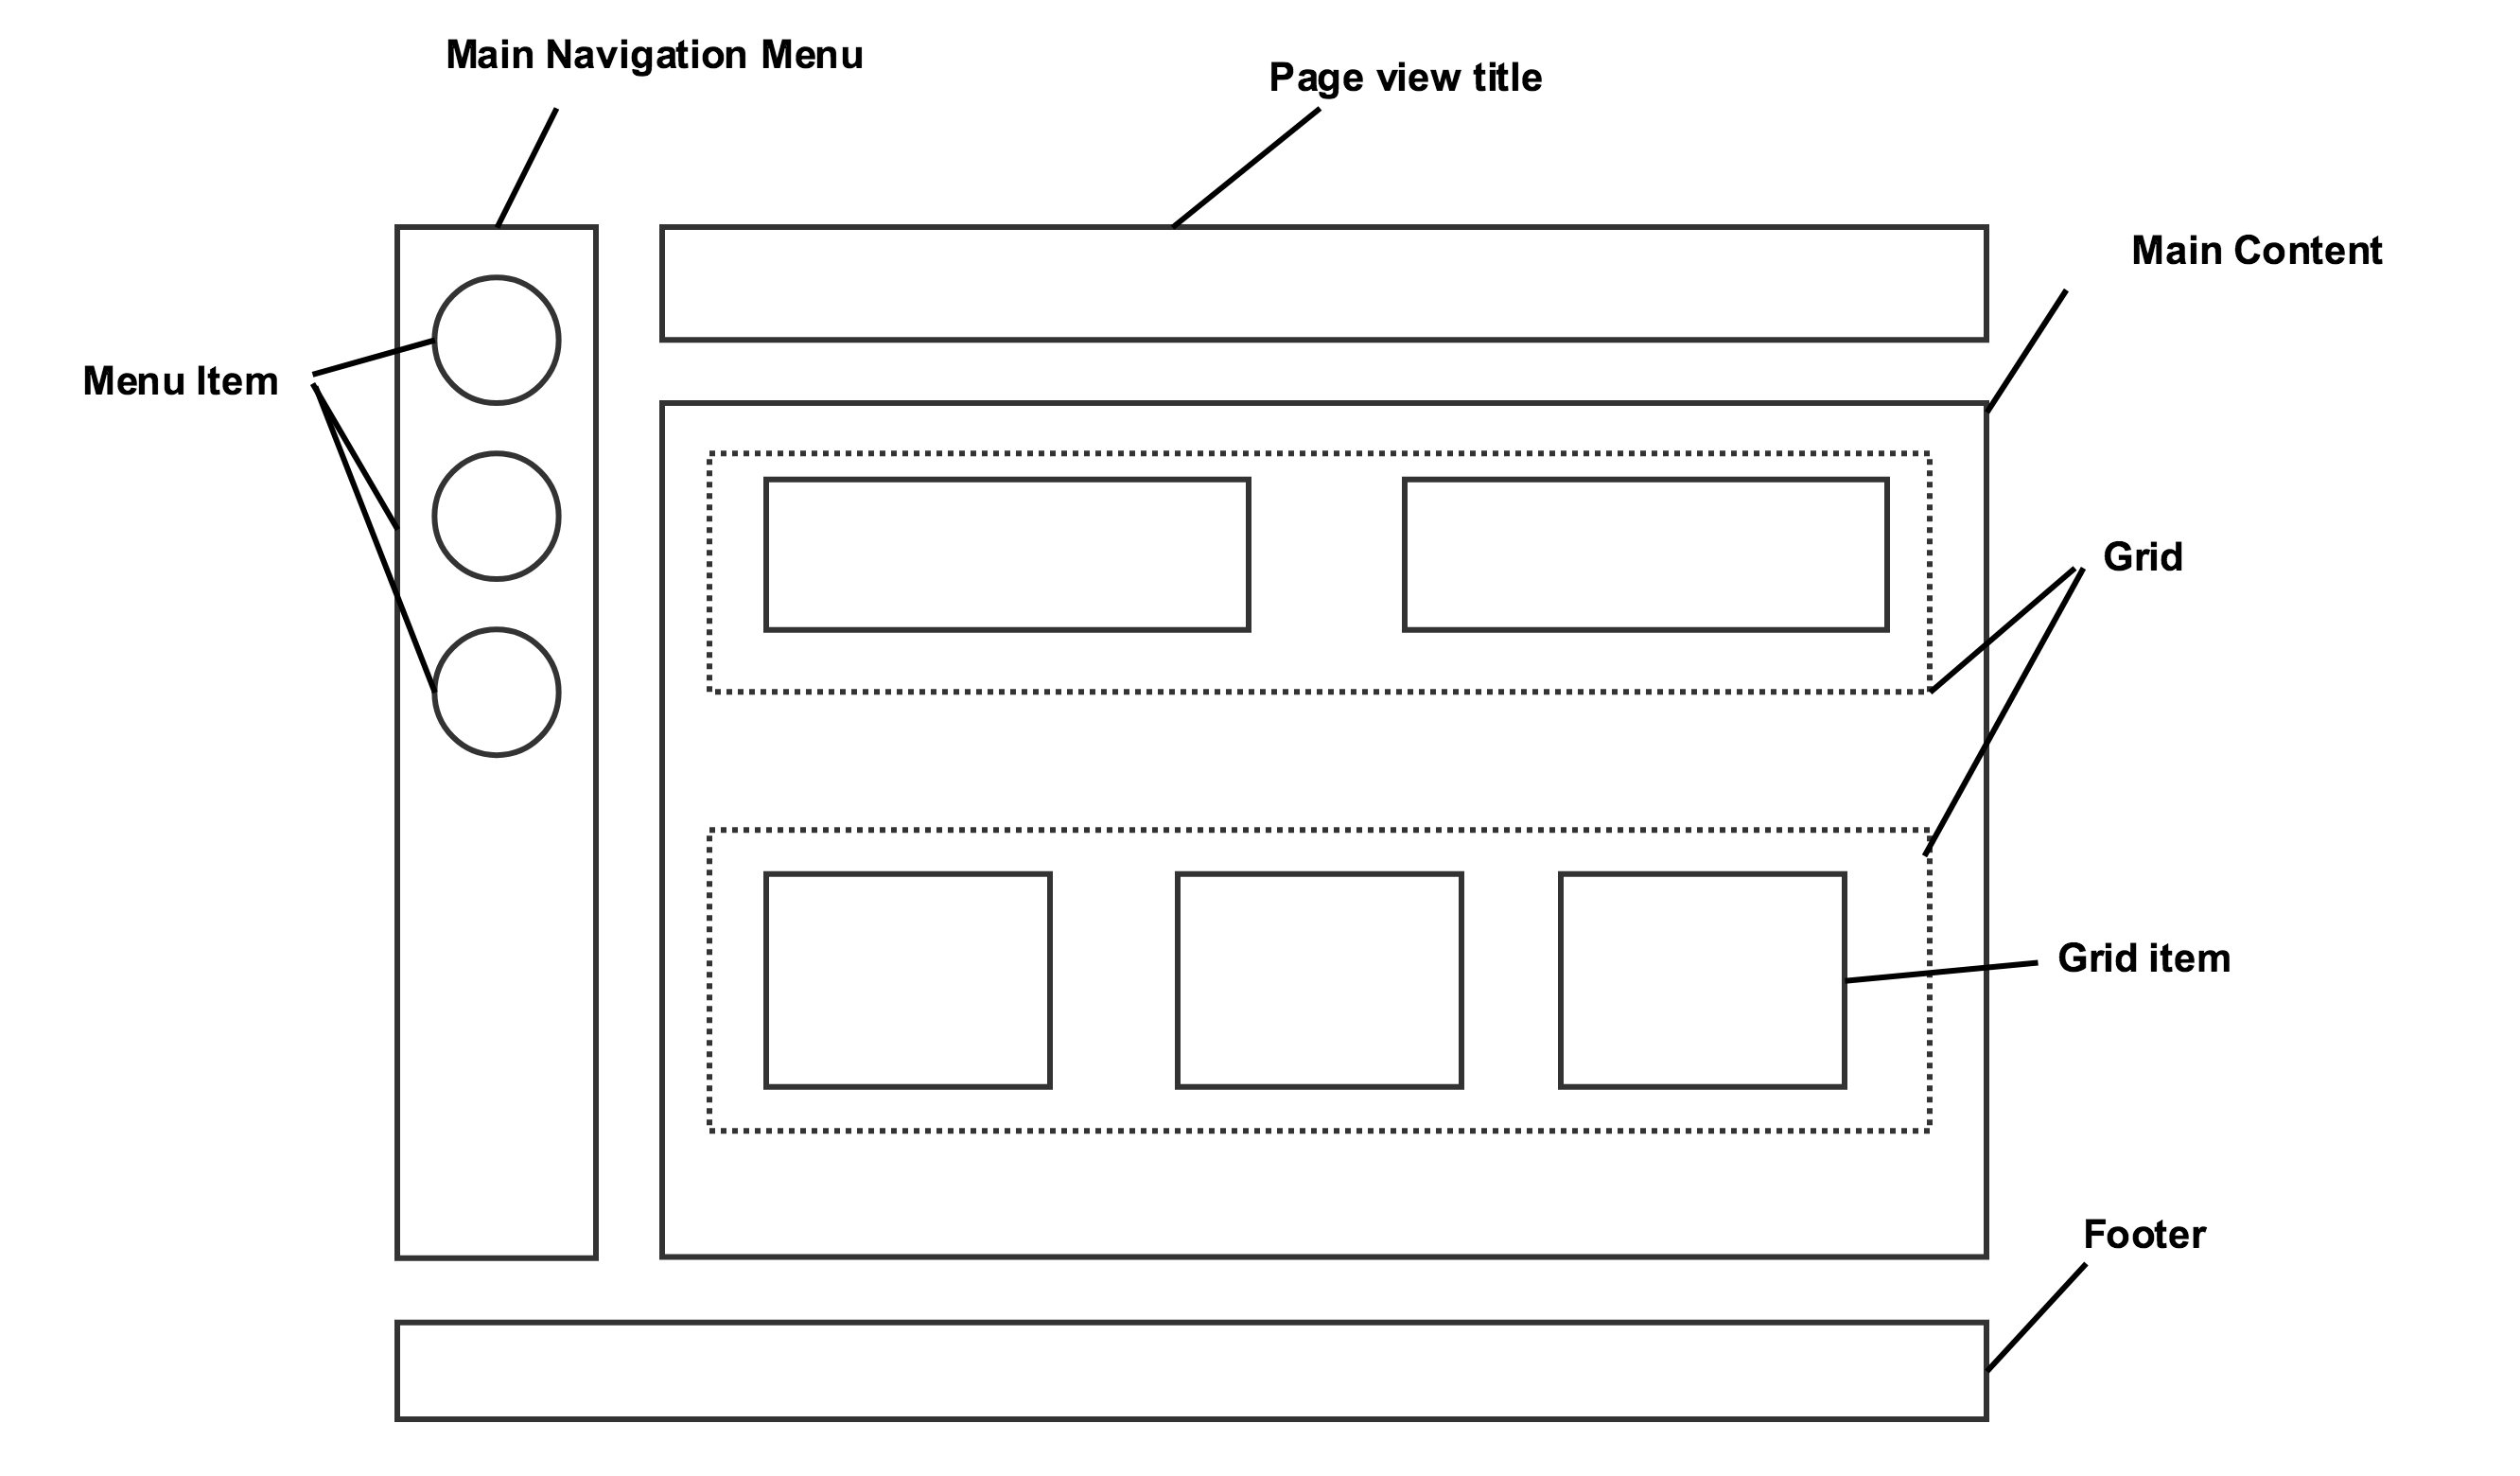
\includegraphics[width=\linewidth]{components/3/components/layout_main.png}
  \caption{N2Sky Main Layout}
  \label{fig:layout_main}
\end{center}
\end{figure}

\begin{itemize}
\item Main Navigation Menu, which displayed as a vertical bar. This component has two states: on mouse over it will be extended and menu items with a caption text and icon will appear, on mouse away from the component only menu items icon will be displayed. 
\item Menu items are icons with a captions components. Which items will be shown or hidden are depends on user permissions.
\item Grid items are blocking components, which can have multiple sizes but fixed within one grid. The context of grid item can be customized. 
\end{itemize}



\subsubsection{N2Sky Mobile Layout}\label{N2Sky Mobile Layout}

N2Sky supports mobile devices. For mobile devices, the mobile layout was developed as is shown in figure \ref{fig:layout_mobile}.

\begin{figure}[H]
\begin{center}
  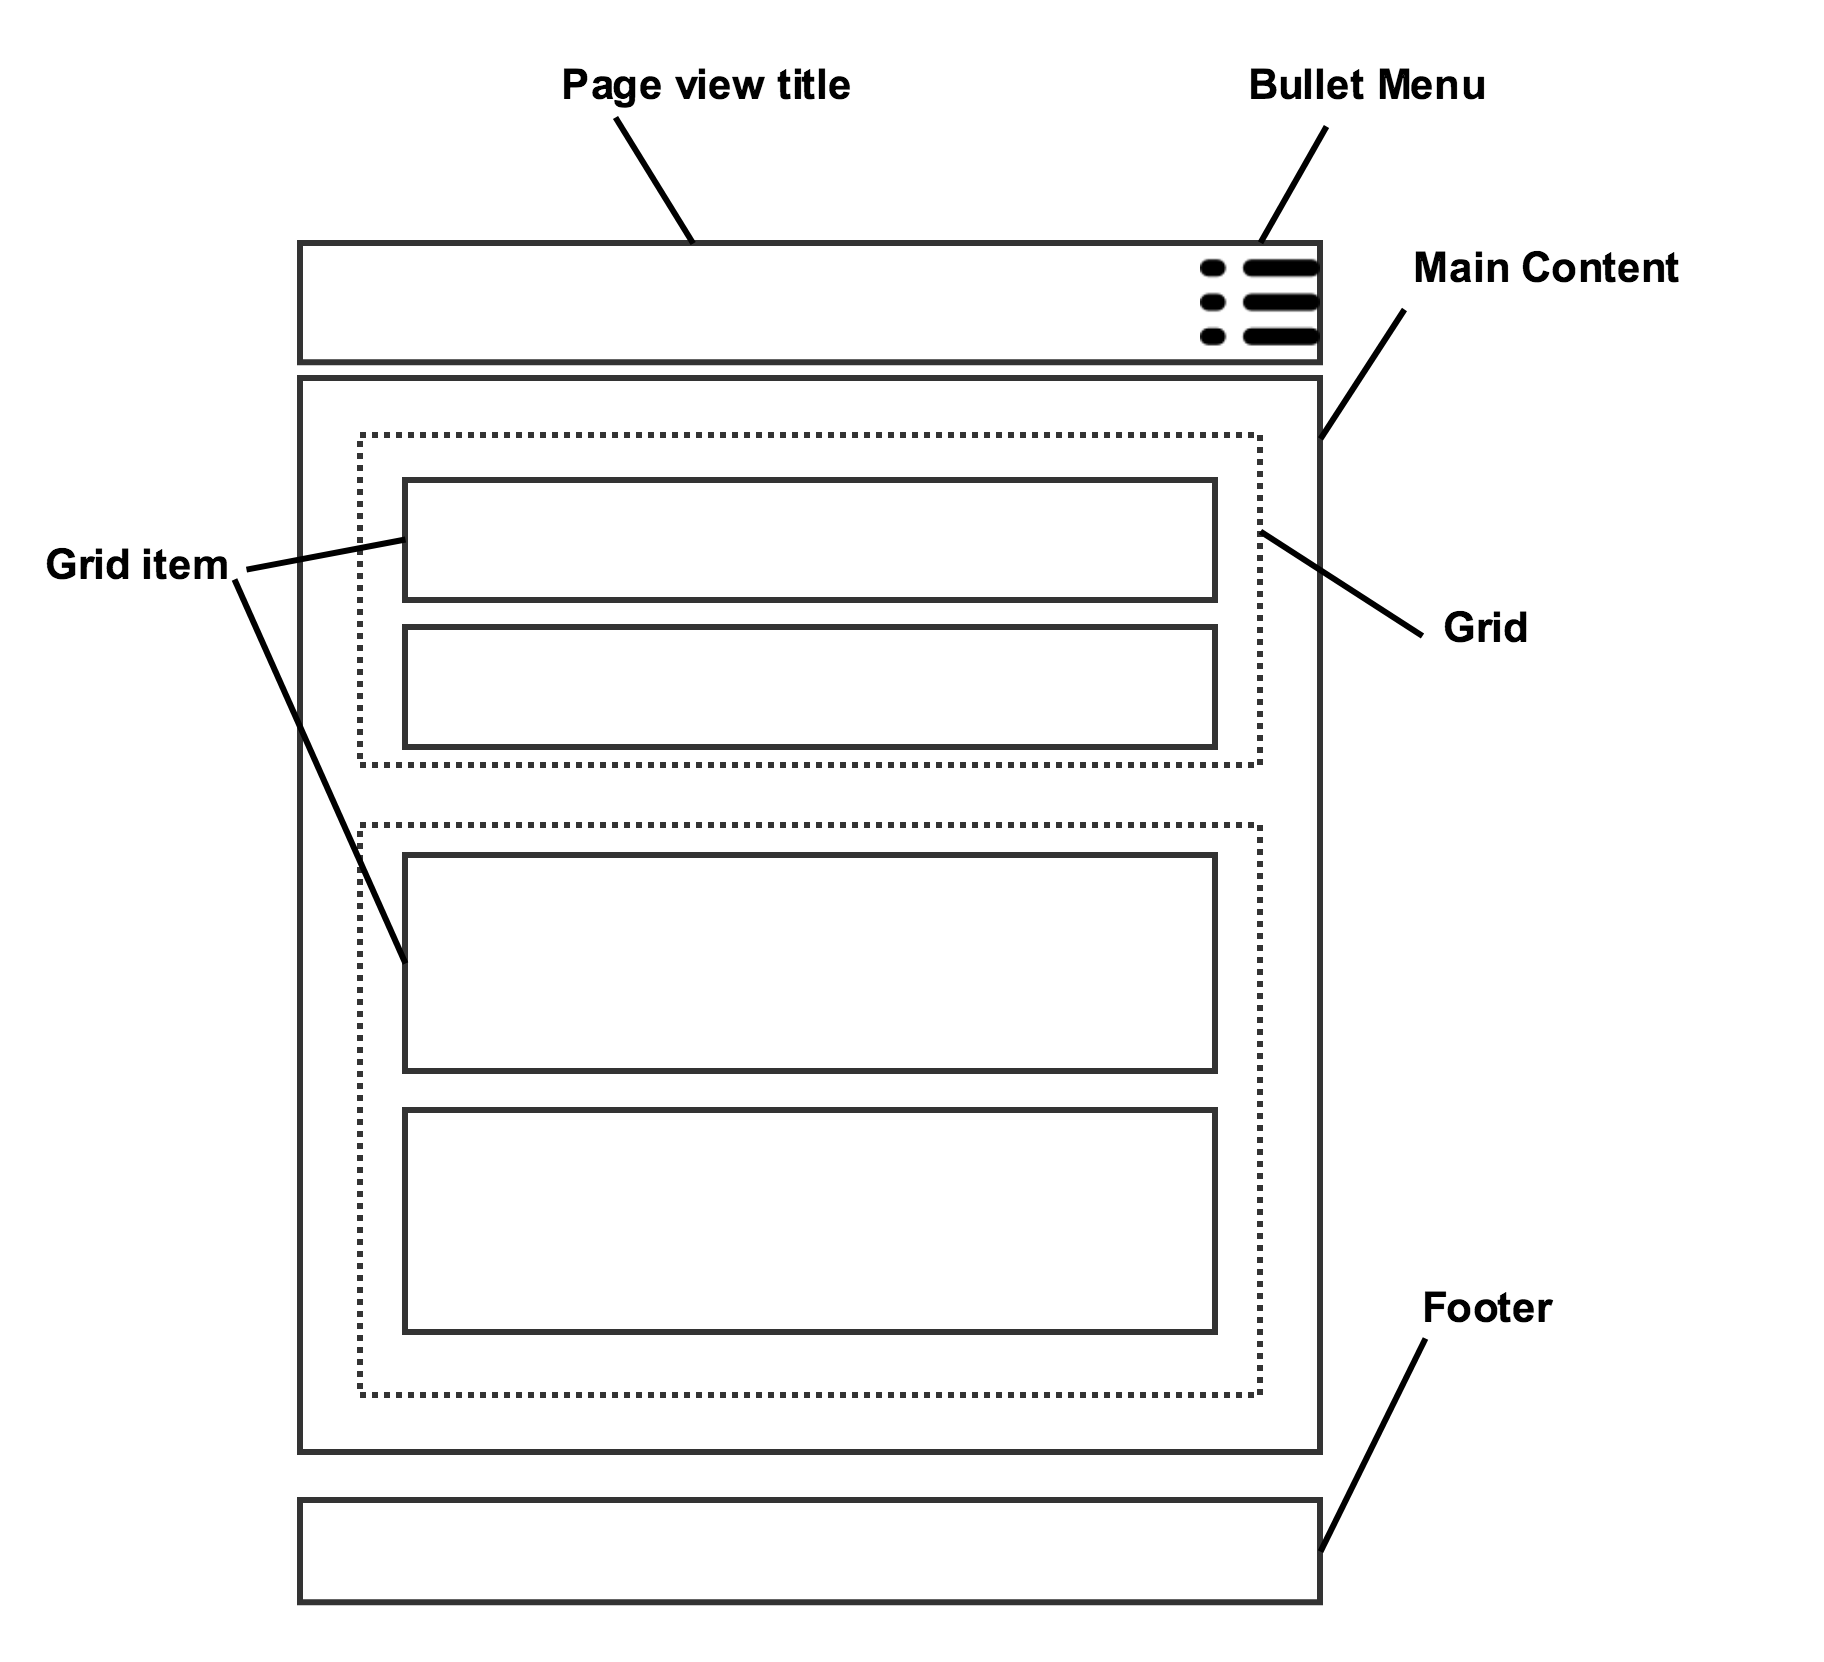
\includegraphics[width=\linewidth]{components/3/components/layout_mobile.png}
  \caption{N2Sky Mobile Layout}
  \label{fig:layout_mobile}
\end{center}
\end{figure}

All components context remain the same, but the positioning is changed. All grid items are vertically located and the width of grid items are the same as the device screen size. 

Additionally next to page view title component is Bullet Menu located. The normal desktop view is hidden and instead bullet menu perform the same functionality. On mouse click, the menu will appear as an overlay of the current view. 

\subsubsection{N2Sky Page Views}\label{N2Sky Page Views}

As it was mentioned in \autoref{Technology Stack} "Technology Stack", N2Sky frontend application developed on the ReactJS framework. Part of the ReactJS framework is React-Router, which contains all page views of the application and redirects it accordantly to URL path:

\begin{lstlisting}
<Provider store={store}>
	<Router history={browserHistory}>
		<Route path="/" component={Auth}/>
		<Route path="/signup" component={Reg}/>
		<Route component={AbstractDashboardLayout}>
			<Route path="/cloud" component={DashboardsOverview}/>
			<Route path="/user/profile" component={UserProfile}/>
			<Route path="/openstack" 
				component={OpenStackMainDashboard}/>
			<Route path="/openstack/project/:id"
				 component={OpenStackProjectDashboard}/>
			<Route path="/openstack/server/:projectid/:serverid" 
				component={ServerDetailsDashboard}/>
			<Route path="/openstack/vitrage/:templateId" 
				component={VitrageDetailsView}/>
			<Route path="/alert" component={AlertDashboard}/>
		</Route>
		<Route component={AbstractDashboardLayout}>
			<Route path="/n2sky" component={N2SkyDashboard}/>
			<Route path="/n2sky/available"
				 components={AvailableNetworksOverview}/>
			<Route path="/n2sky/models" 
				components={ModelsRepository}/>
			<Route path="/n2sky/paradigm/create/:projectid" 
				components={AddNNFromParadigm} readOnly={false}/>
			<Route path="/n2sky/paradigm/nn/:id" 
				components={AddNNFromParadigm} readOnly={true}/>
			<Route path="/n2sky/network/:id" 
				component={NetworkDetails}/>
			<Route path="/n2sky/network/:id/test/:model_id"
				 component={NetworkTestDetails}/>
			<Route path="/n2sky/project/:id"
				component={ProjectDashboard}/>
		</Route>
	</Router>
</Provider>
\end{lstlisting}

Every "Route" is a page view redirector and contains:
\begin{itemize}
\item Path, which responsible for URL redirection.
\item Component, which is a page view itself
\item Other props, which are optional
\end{itemize}

As it was mentioned in \autoref{Modular frontend application design} "Modular frontend application design", N2Sky contains two modules: Administration module and main application module. Both of this module sharing the same main application layout and having following page views: 
\begin{itemize}
\item \textbf{Administration Module:}
\begin{description}
\item[Cloud Dashboard View, path: "/cloud".] It is the main dashboard of Administration module, which contains overview dashlets of every modules component.
\item[OpenStack Dashboard View, path: "/openstack".] This view contains all information about OpenStack and the main control center of the OpenStack services.
\item[OpenStack Project, path: "/openstack/project/:id".] Route to the OpenStack project, which contains information about servers, flavours, images etc. of the particular project. In path "id" is the id of OpenStack project.
\item[Server Details View, path: "/openstack/server/:projectid/:serverid".] This view contains information about OpenStack instance. The URL path needs OpenStack project id and the id of the OpenStack instance. 
\item[Vitrage Details View, path: "/openstack/vitrage/:templateId".] Vitrage it a monitoring service of OpenStack and its instances. This view contains information about this service. The template id is required.
\item[Alert Management Dashboard View, path: "/alert".]  This view is a dashboard of Alert Management System. This view contains information about alerting rules and alerting events.
\end{description}

\item \textbf{Main Application Module:}
\begin{description}
\item[Authentication View, path: "/".] First page, which user sees, when he loading the application.  Authentication View contains login form.
\item[Registration View, path: "/signup".] Registration View contains registration form.
 \item[N2Sky Dashboard, path: "/n2sky".] Main Application Module view is the N2Sky Dashboard. This view contains information about logged in user projects, neural networks and trained models.  
\item[Available Networks View, path: "/n2sky/available".] This view is the neural network repository of the N2Sky. It is possible to copy available neural networks to own project.
\item[Models Repository View, path: "/n2sky/models".] The trained neural network are showed in this view. It is possible to copy published models to own project.
\item[Neural Network Create View, path: "/n2sky/paradigm/create/:projectid".] This view represents workflow of the creation of neural network from existing paradigm. The newly created neural network will be saved in user's project, hence this project id is required.  
\item[Neural Network Details View, path: "/n2sky/network/:id".] The details of the created neural network. It can be as well logged in user neural network or neural network from another user. User permissions show visibility level. The networks id is required. 
\item[Neural Network Test View, path: "/n2sky/network/:id/test/:model\_id".] From this view user can evaluate neural network this his own input parameters. Neural network id and trained model id are required. 
\item[Project Dashboard View, path: "/n2sky/project/:id".] This view shows the neural networks and models, which were created in particular project. The project id is required.
\end{description}


\end{itemize}






\subsubsection{N2Sky Dashboards}\label{N2Sky Dashboards}

The purpose of the dashboard is to embed business intelligent (BI) objects into the single page in order to make an overview of highlighted titles of BI objects \cite{dashboards_book}.

A dashboard has a structure layer upon its dashlets. It allows the user to manage layout and properties of dashlets. A dashboard is composed of dashlets. Every dashlet contains specific context and data. Dashboard defines: 
\begin{itemize}
\item Dashlets to be displayed
\item The layout of dashboard and positioning of its dashlets
\item The common context of particular dashlets
\end{itemize}


\begin{figure}[H]
\begin{center}
  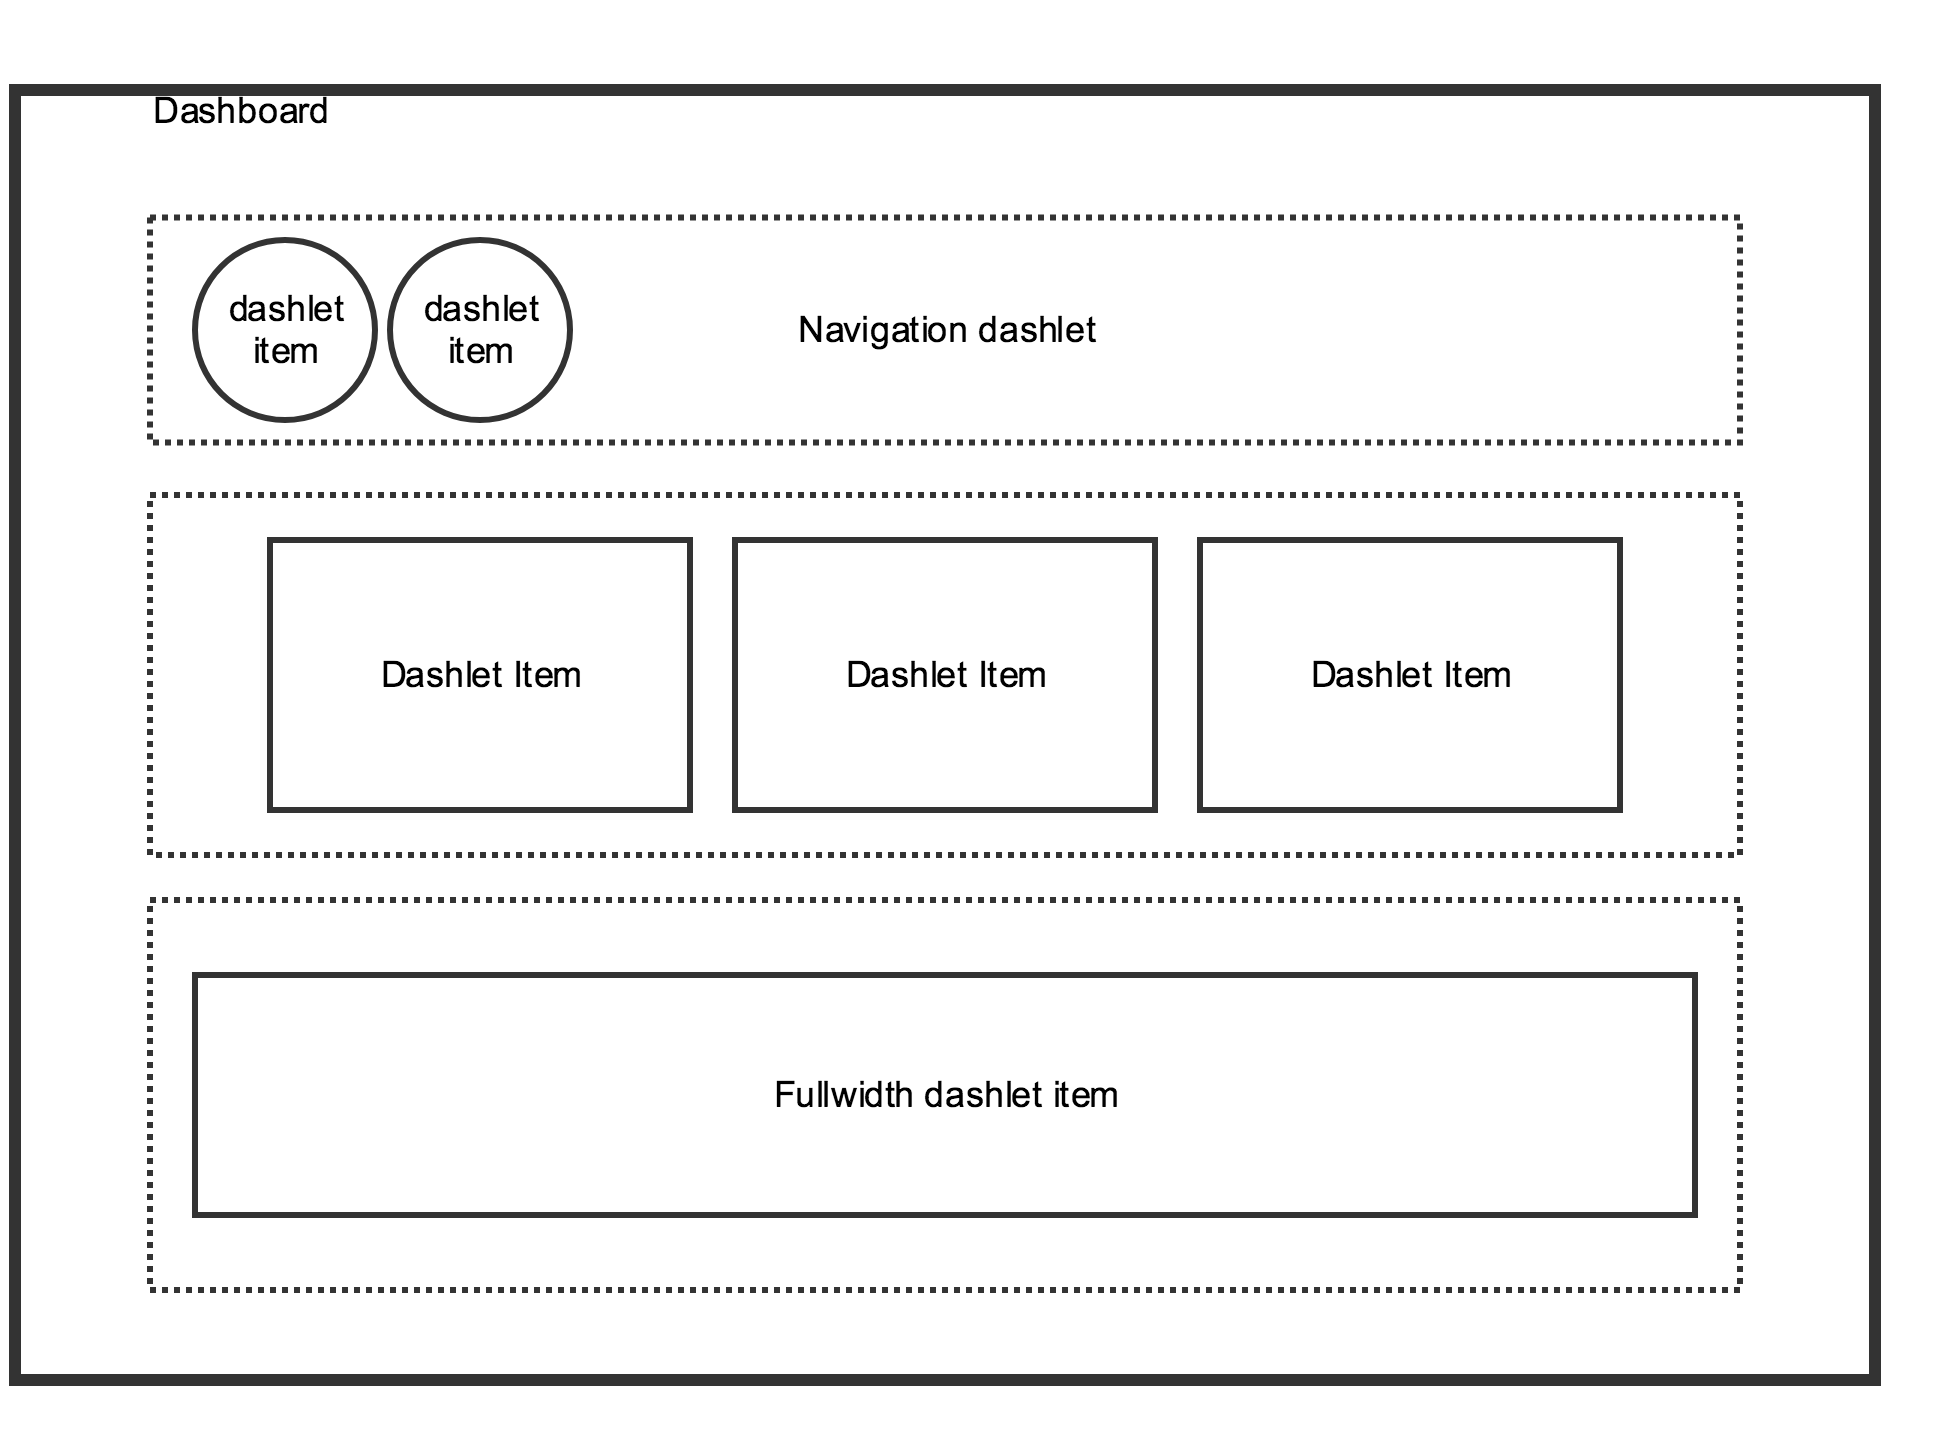
\includegraphics[width=\linewidth]{components/3/components/dashboard_template.png}
  \caption{N2Sky Dashboard template}
  \label{fig:dashboard_template}
\end{center}
\end{figure}

In the figure \ref{fig:dashboard_template} is shown the typical N2Sky dashboard template. A dashboard in N2Sky has a grid structure. Every dashlet has one or more items. Every item can contain any UI component, but it has to be feet into assigned dashlet without overlays. 



\subsubsection{Responsive design}\label{Responsive design}

Since N2Sky is cross-platform application it has to support multiple screen resolutions as well as readability and usability. 

Considering readability first of all the typography has to be mentioned. During development of N2Sky to find the fonts, which will be displayed same and will be readable across multiple devices was a challenge. The typeface \cite{wiki:typeface} properties like latter spacing, width, weight etc were adjusted multiple times. The common problem was to audit how typeface represents on mobile devices and desktop computers \cite{responsive_book}. Even such a standard fonts like "Arial" and "Times New Roman" were looking unreadable on mobile devices as it is shown in figure \ref{fig:typo}.

\begin{figure}[htbp]
\begin{center}
  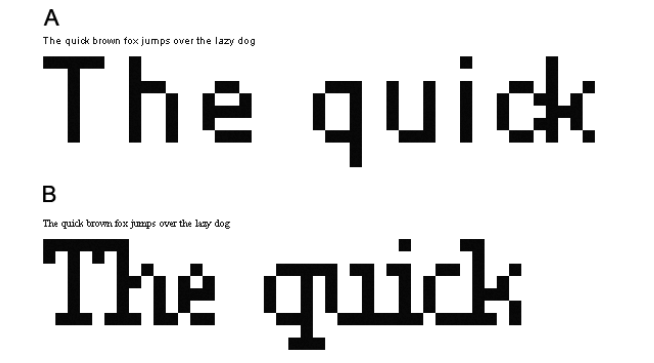
\includegraphics[scale=0.5]{components/3/components/typo.png}
  \caption{Difference between sans-serif font Arial (A) and the browser serif font Times New Roman (B) }
  \label{fig:typo}
\end{center}
\end{figure}

The expansion of cross-platform applications brought some freedom to developers and designers. Today is possible to develop an application simultaneously for mobile devices, desktop computers, and web browsers. The problem comes, when the mobile and tablet devices manufacturers started to produce devices with different resolutions. Today versioning of mobile screen resolution came over 1000 devices, but N2Sky was concentrating only on major market players as it is shown in figure \ref{fig:screen} \cite{mobile_resolution}.

\begin{figure}[htbp]
\begin{center}
  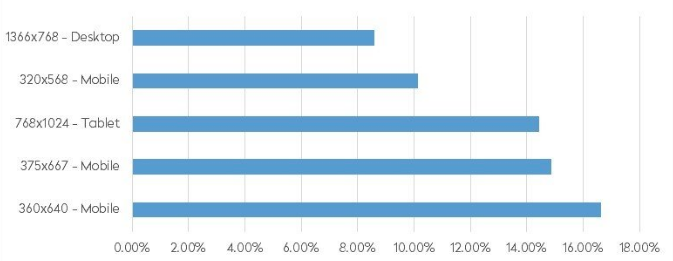
\includegraphics[scale=0.65]{components/3/components/screen.png}
  \caption{Average screen resolution of mobile, tablet and desktop devices on 2017}
  \label{fig:screen}
\end{center}
\end{figure}

N2Sky is focused on mobile and tablet devices because it is an extensive trend nowadays. 

\subsubsection{User Interface Elements}\label{User Interface Elements}

It is possible to divide all UI elements into groups \cite{intelligent_support}:

\begin{description}
\item[Input Controls.] Input controls determine user input action. Input actions are keyboard typing or mouse clicking.  Following UI elements are the part of input controls: 
\begin{itemize}
\item Checkboxes
\item Radio buttons 
\item Dropdown Lists
\item List boxes
\item Buttons
\item Toggles
\item Text fields
\item Date field
\end{itemize}
\item[Navigational Components.] Navigation between page views. Navigational components include also some particular request from and to the user. Following UI elements are the parts of navigational components:
\begin{itemize}
\item Breadcrumb 
\item Slider
\item Search field
\item Pagination
\item Slider
\item Tags
\item Icons
\end{itemize}
\item[Informational Components.] These components are the addition to workflows. It can help the user to perform some actions or they can inform the user, that the action will occur or already occurred. Informational Components contains following UI elements:
\begin{itemize}
\item Tooltips
\item Icons
\item Progress bar
\item Notifications
\item Message boxes
\item Modal windows
\end{itemize}
\item[Containers.] Containers are components, which are hiding additional information or not focused information, where the user needs to perform the action in order to see it.   
\begin{itemize}
\item Accordion
\item Semi-hidden elements
\end{itemize}
\end{description}

\subsubsection{UI Elements in N2Sky}\label{UI Elements in N2Sky}

N2Sky supports almost all common web user interface elements. Every element was developed in order to be reusable. Since N2Sky supports responsive design, the UI elements should also be responsive. Every UI element is absolute customised. Following UI elements were created:

\begin{description}
\item[Accordion]  Accordion is a list of items, which is accessible on mouse click. In N2Sky accordion works more like a modal window. With this kind of functionality other data, which surround accordion will not be stretched or squeezed but will appear on top of elements as it is shown in figure \ref{fig:accordion}: 

\begin{figure}[htbp]
\begin{center}
  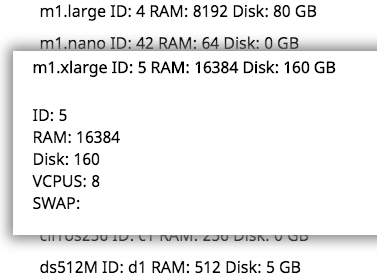
\includegraphics[scale=0.75]{components/3/components/accordion.png}
  \caption{Customised N2Sky accordion UI element}
  \label{fig:accordion}
\end{center}
\end{figure}

\item[Buttons.] Idea behind was to make buttons more interactive and understandable to use as it is displayed in \ref{fig:button_inactive}. Buttons contain caption and icon in SVG format in order to support high quality image in all devices.

Buttons are using on hover animation. When mouse over the button, then button icon slide to the middle to show that action can be performed as it is shown in figure \ref{fig:button_active}. 

\begin{figure}[htbp]
\begin{center}
  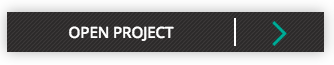
\includegraphics[scale=0.55]{components/3/components/button_inactive.png}
  \caption{Customised N2Sky button UI element}
  \label{fig:button_inactive}
\end{center}
\end{figure}


\begin{figure}[htbp]
\begin{center}
  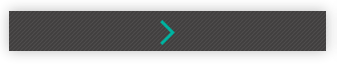
\includegraphics[scale=0.55]{components/3/components/button_active.png}
  \caption{Customised N2Sky button UI element animation}
  \label{fig:button_active}
\end{center}
\end{figure}

\item[Icons.] In N2Sky all icons are in Scalable Vector Graphics (SVG) format. With SVG the icons do not lose quality in any device \cite{Cagle2005}. Since it is a vector graphic it easy to edit an icon with programming language code. N2Sky Logo, which is represented in figure \ref{fig:logo},  is also made in SVG format. 

\begin{figure}[htbp]
\begin{center}
  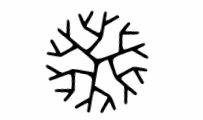
\includegraphics[scale=0.55]{components/3/components/logo.png}
  \caption{Customised N2Sky logo in SVG format}
  \label{fig:logo}
\end{center}
\end{figure}

Is it possible to import code in some graphical vector editor in order change color, path (vector graphic itself), metadata etc. Following code demonstrate N2Sky Logo in SVG format. The whole vector path was shortened.

\begin{lstlisting}
<?xml version="1.0" standalone="no"?>
<!DOCTYPE svg PUBLIC "-//W3C//DTD SVG 20010904//EN"
        "http://www.w3.org/TR/2001/REC-SVG-20010904/DTD/svg10.dtd">
<svg version="1.0" xmlns="http://www.w3.org/2000/svg"
     width="266.000000pt" height="267pt" viewBox="0 0 266 267"
     preserveAspectRatio="xMidYMid meet">
    <metadata>
        N2Sky Logo. 2018
    </metadata>
    <g transform="translate(0.000000,267.000000) scale(0.100000,-0.100000)"
       fill="#6b6b6b" stroke="none">
        <path d="M1302 2638 c-9 -9 -12 -83 -12 -270 0 -245 -1 -259
-37 -26 -170 21 -63 23 -132 46 -152 52 -23 7 -38 17 -38 27 1
80 222 90 255 87 284 -2 23 -9 32 -25 34 -27 4 -46 -23 -72 -106 
-77 -34 -95 -8 -18 -22 -51 -32 -74 -10 -24 -21 -43 -25 -43 -5 0 -30 
76 -76 118 -100 136 -128 92 -12 -20 -10 -26 101 -219 35 -60 109 

...

-18 74 -40 36 -22 67 -40 70 -40 11 0 253 -152 269 -169 11 -12 15 -27 12 
-36 26 -103 -14 -32 -19 -60 -35 -62 -35 -3 0 -34 -18 -70 -40 -36 -22 -68
-40 -70 -40 -3 0 -22 -11 -43 -23 -142 -90 -172 -96 -201 -39 -20 40 -47 168
-55 268 l-5 61 122 22 c67 13 156 30 197 38 85 16 106 30 95 63 -7 21 -11 22
-69 16 -33 -4 -88 -10 -121 -15 -178 -26 -178 -26 -170 -1 4 13 21 46 37 74
57 100 63 116 52 134 -6 9 -22 17 -34 17 -24 0 -47 -33 -130 -180 -75 -132
-74 -130 -61 -206 6 -38 16 -102 21 -141 6 -40 15 -98 20 -129 6 -30 10 -72
10 -93 l0 -38 -162 4 c-151 3 -167 5 -212 28 -82 43 -86 57 -86 320 l0 226 38
34 c21 19 53 47 72 61 19 14 49 39 67 55 17 16 54 47 82 69 60 49 79 79 65
103 -18 28 -47 25 -84 -10 -20 -18 -52 -45 -72 -60 -20 -15 -42 -34 -50 -41
-23 -23 -92 -67 -105 -67 -10 0 -13 27 -13 104 0 57 -3 111 -6 120 -7 19 -45
21 -62 4z"/>
    </g>
</svg>
\end{lstlisting}

\item[Notification messages.] Notification messages are the part of information component. In N2Sky used two types of notification messages: 
\begin{itemize}
\item Waring message, which tells, that something goes wrong as it shown in ``Fig.~\ref{fig:notif_warning}''. It can be an error in the application as well as user workflow error. 
\item Informational message that gives information about the event which will occur or already occurred as it shown in ``Fig.~\ref{fig:notif_info}''.
\end{itemize}


\begin{figure}[htbp]
\begin{center}
  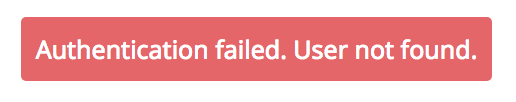
\includegraphics[scale=0.65]{components/3/components/notif_warning.png}
  \caption{Customised N2Sky warning message UI element}
  \label{fig:notif_warning}
\end{center}
\end{figure}

\begin{figure}[htbp]
\begin{center}
  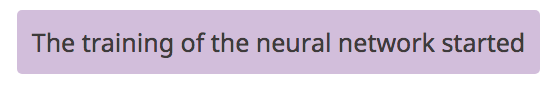
\includegraphics[scale=0.65]{components/3/components/notif_info.png}
  \caption{Customised N2Sky informational message UI element}
  \label{fig:notif_info}
\end{center}
\end{figure}

\item[Navigation.] In N2Sky user can navigate to another one page or change part of the page view via tabs, navigation buttons, and menus. 
Navigation elements are bind to the group of element or UI components. Following navigation component which is shown in ``Fig.~\ref{fig:nav}'', contains navigation elements as well functional icon. 
\end{description}

\begin{figure}[htbp]
\begin{center}
  
\includegraphics[scale=0.65]{components/3/components/nav.png}
  \caption{Customised N2Sky navigation UI element}
  \label{fig:nav}
\end{center}
\end{figure}

Navigation bars can contain tabs, buttons, icons and non-functional text. ``Fig.~\ref{fig:nav_bar}'' shows navigation bar an custom table. 

\begin{figure}[htbp]
\begin{center}
  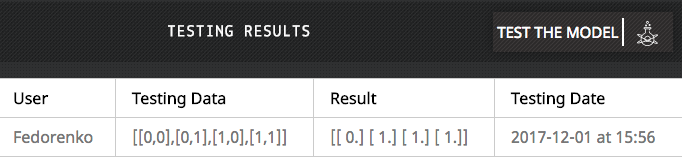
\includegraphics[scale=0.65]{components/3/components/nav_bar.png}
  \caption{Customised N2Sky navigation bar with a table}
  \label{fig:nav_bar}
\end{center}
\end{figure}

\subsubsection{UI Components in N2Sky}\label{UI Components in N2Sky}

Groups of UI elements form UI components. Components, like elements, are also fully reusable, the only context of components is changing. Following custom UI components were developed in N2Sky: 

\begin{description}
\item[Grid Item Component.] Grid in N2Sky is responsive. It can change positions and size of grid items like it shown in ``Fig.~\ref{fig:grid_item}''. 

\begin{figure}[htbp]
\begin{center}
  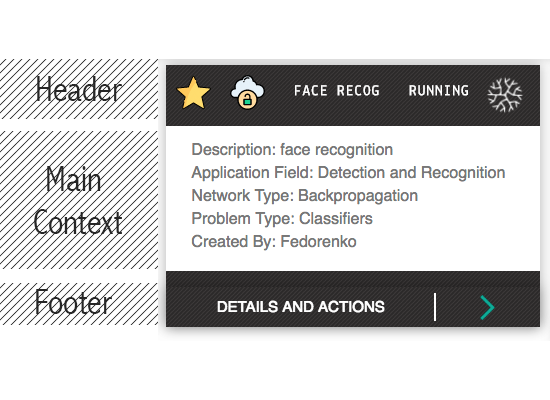
\includegraphics[scale=0.65]{components/3/components/grid_item.png}
  \caption{Responsive N2Sky Grid Item UI comonent}
  \label{fig:grid_item}
\end{center}
\end{figure}


Grid item contains following UI element: 
\begin{description}
\item[Header. ] Header is the first component on which the user focuses, that is why it should be short but highlighted. Following UI elements are included: 
\begin{itemize}
\item Functional icons-buttons on the left side (optional)
\item Title of grid item (mandatory)
\item  Non-functional icons (optional)
\end{itemize}
\item[Main context. ] Component, which contains context information. This component can be fully customized. It is possible to put there the list of items, plain text or even image.
 \item[Footer. ] Footer is an optional element and contains only button UI element. 
\end{description}

\item[Main navigation menu.] Every N2Sky view use main navigation menu, namely, the menu is injected in an abstract view, which is extended by all other view components. The menu has menu items, which contain caption and an icon. As it was mentioned before, N2Sky has two modules: administration module and main application module. Both modules are represented in menu and menu items visibility depending on logged-in user permission. 
Menu for arbitrary user is shown in figure \ref{fig:menu_user}  and has following menu items:

\begin{itemize}
\item Profile 
\item N2Sky Dashboard
\item Available neural networks
\item Models repository
\end{itemize}

 
 \begin{figure}[htbp]
\begin{center}
  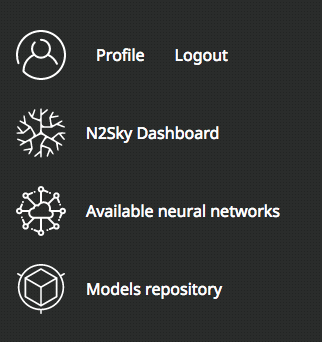
\includegraphics[scale=0.65]{components/3/components/menu_user.png}
  \caption{N2Sky Main Navigation Menu for arbitrary user}
  \label{fig:menu_user}
\end{center}
\end{figure}

If end-user is a system administrator, he can see additional menu form administration module as is demonstrated in ``Fig.~\ref{fig:menu_admin}'. This menu contains dropdown submenus: 

\begin{itemize}
\item OpenStack Dashboard
\item Cloudify Dashboard
\item Alert System
\item Dashboards Settings
\end{itemize}


 \begin{figure}[htbp]
\begin{center}
  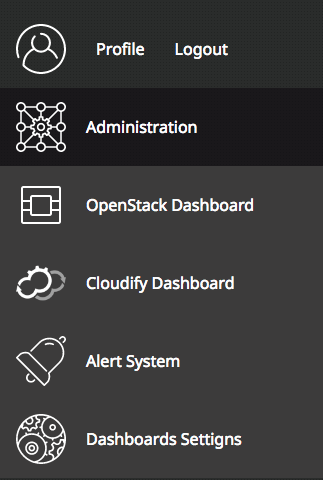
\includegraphics[scale=0.65]{components/3/components/menu_admin.png}
  \caption{N2Sky Main Navigation Menu for system administrator}
  \label{fig:menu_admin}
\end{center}
\end{figure}

\item[Modal windows.] N2Sky use modal windows almost in every view as it is shown in figure \ref{fig:modal}. Modals are responsive and touch screen friendly. It has 3 elements:
\begin{itemize}
\item Title (mandatory)
\item Context (mandatory)
\item Submit button (optional)
\end{itemize}

 \begin{figure}[H]
\begin{center}
  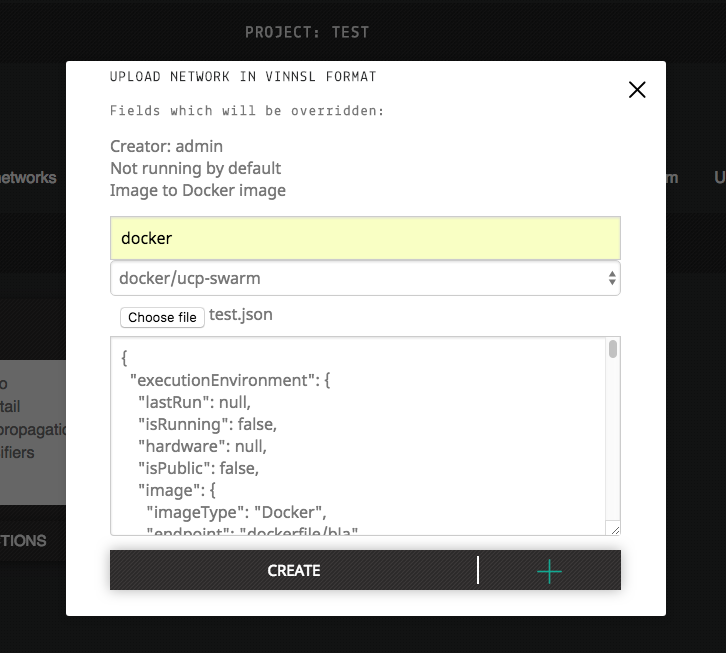
\includegraphics[scale=0.5]{components/3/components/modal.png}
  \caption{N2Sky Modal Window UI component}
  \label{fig:modal}
\end{center}
\end{figure}

Modals can be used to represent form as well for informational purposes. When modal is open the background is dunned in order to focus the user on modal context. The modal context itself can be fully custom. It is possible to put any UI element in context.



\end{description}



\subsection{N2Sky Services}\label{N2Sky Services}

 N2Sky implements the microservices architecture. It has 3 main web services as it is shown in figure \ref{fig:newarch}:
 
\begin{itemize}
\item User Management Web Service
\item Model Repository Web Service
\item Cloud management Web Service
\end{itemize}

Every web service uses other services which are not exposed to the public. It was made in order to support application encapsulation. Encapsulation of web application helps to prevent security issue. One of the crucial crucial processes in N2Sky is the neural network training. This process takes almost all resources of the environment, that is why it is not exposed. Such a process can be triggered only by web service, which can be blocked if the environment is overloaded.

Consider the following web services in details and which processes and services they are encapsulated:  


\subsubsection{User Management Web Service.}\label{User Management Web Service}   This web service responsible for permissions and user management and it has its own database. The user can authorize in the system and get a session token. Every token is a unique collection of numbers and Latin letters. The token is assigned to the authorized user and will be saved until the user is active. If the user is not active in the next 3 hours, the session token will disappear. If the user still has an active browser session, the authorization token will be revalidated. If user trying to make some illegal request or behave too active, the authorization token will be revoked and the system administrator will be notified of this incident. 

Every user encapsulates permission level. There two different types of permissions:
\begin{itemize}
\item Administrator permission. It means, that the user has full granted permission throw entire application.
\item Regular permission. The user has access only for his own as well as publicly available resources.  
\end{itemize}

 \begin{figure}[H]
\begin{center}
  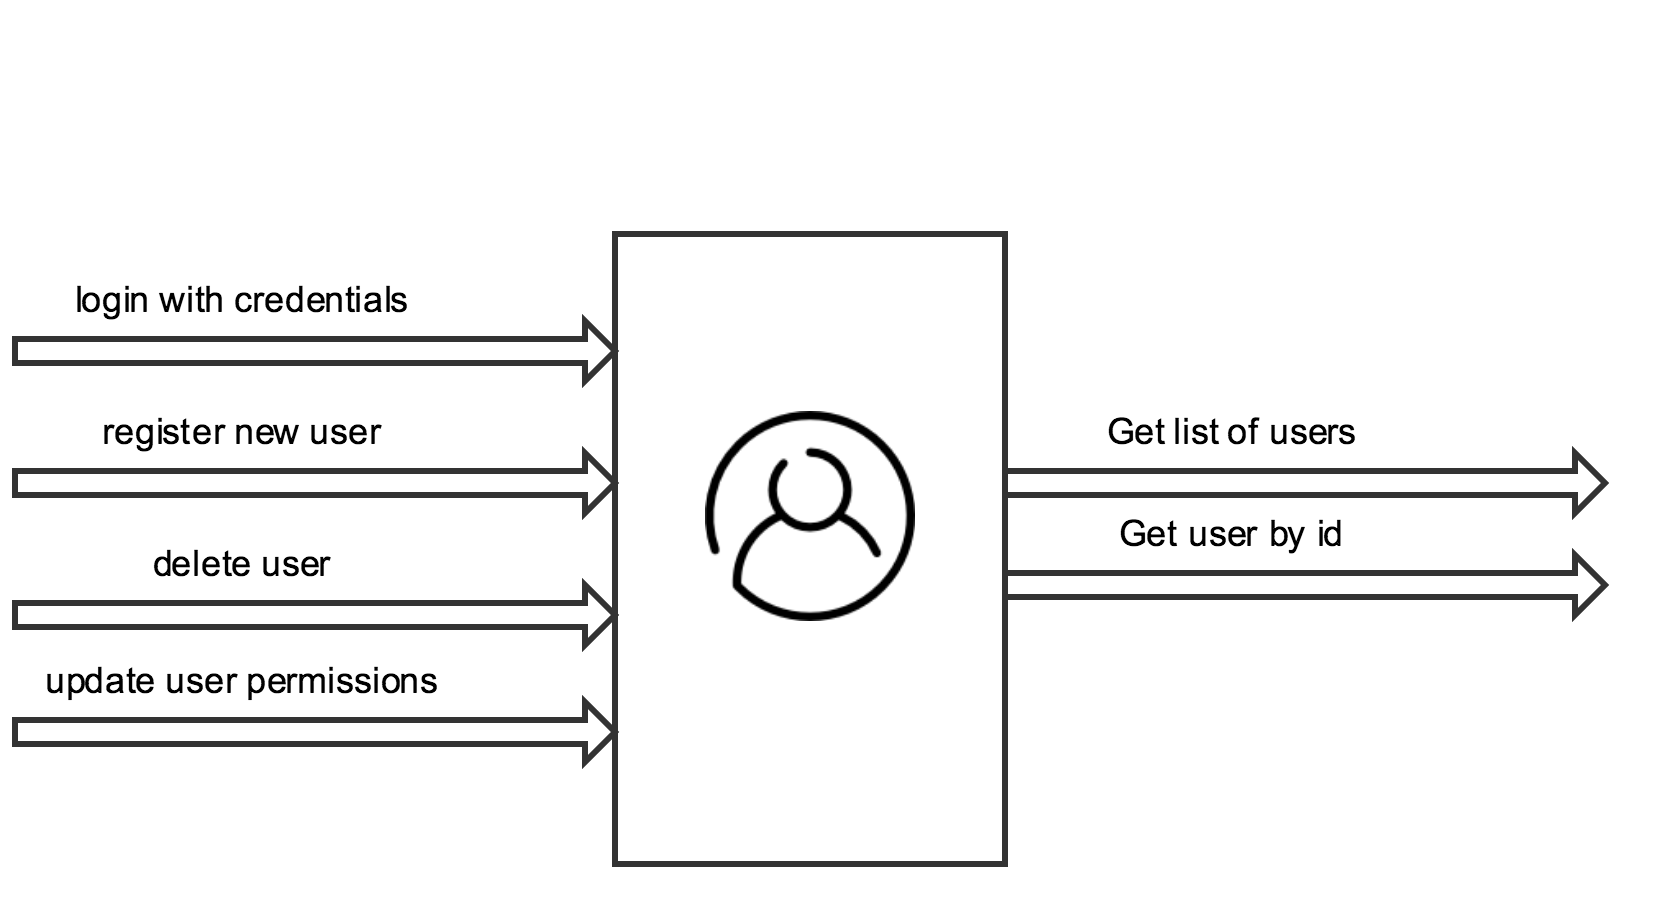
\includegraphics[width=\linewidth]{components/3/components/user_serivice.png}
  \caption{N2Sky User Management Web Service}
  \label{fig:user_serivice}
\end{center}
\end{figure}

As is shown in ``Fig.~\ref{fig:user_serivice}'' User Management Web Service has following accessible services:

\begin{itemize}
\item Login with credentials
\item Register a new user 
\item Delete user
\item Update user permissions
\item Get list of users
\item Get user by user ID
\end{itemize}
 
 Detailed information about web service API and API documentation is written in \autoref{API Documentation}

\subsubsection{Model Repository Web Service.}\label{Model Repository Web Service}  Model Repository Web Service is the core service of N2Sky. The authorized user can create a new project, add their neural network from chose paradigm or deploy own one. Every newly created project is assigned to one user and can not be shared, the only system administrator can look up into other users projects. This functionality also limited by User Management Web Service. 

Using this service user can create a neural network from proposed paradigms as well as upload his own neural network in ViNNSL format \cite{Beran2008}. This functionality exposed via service so that every user can use it either from N2Sky web portal or via HTTP request directly on web service.

\begin{figure}[H]
\begin{center}
  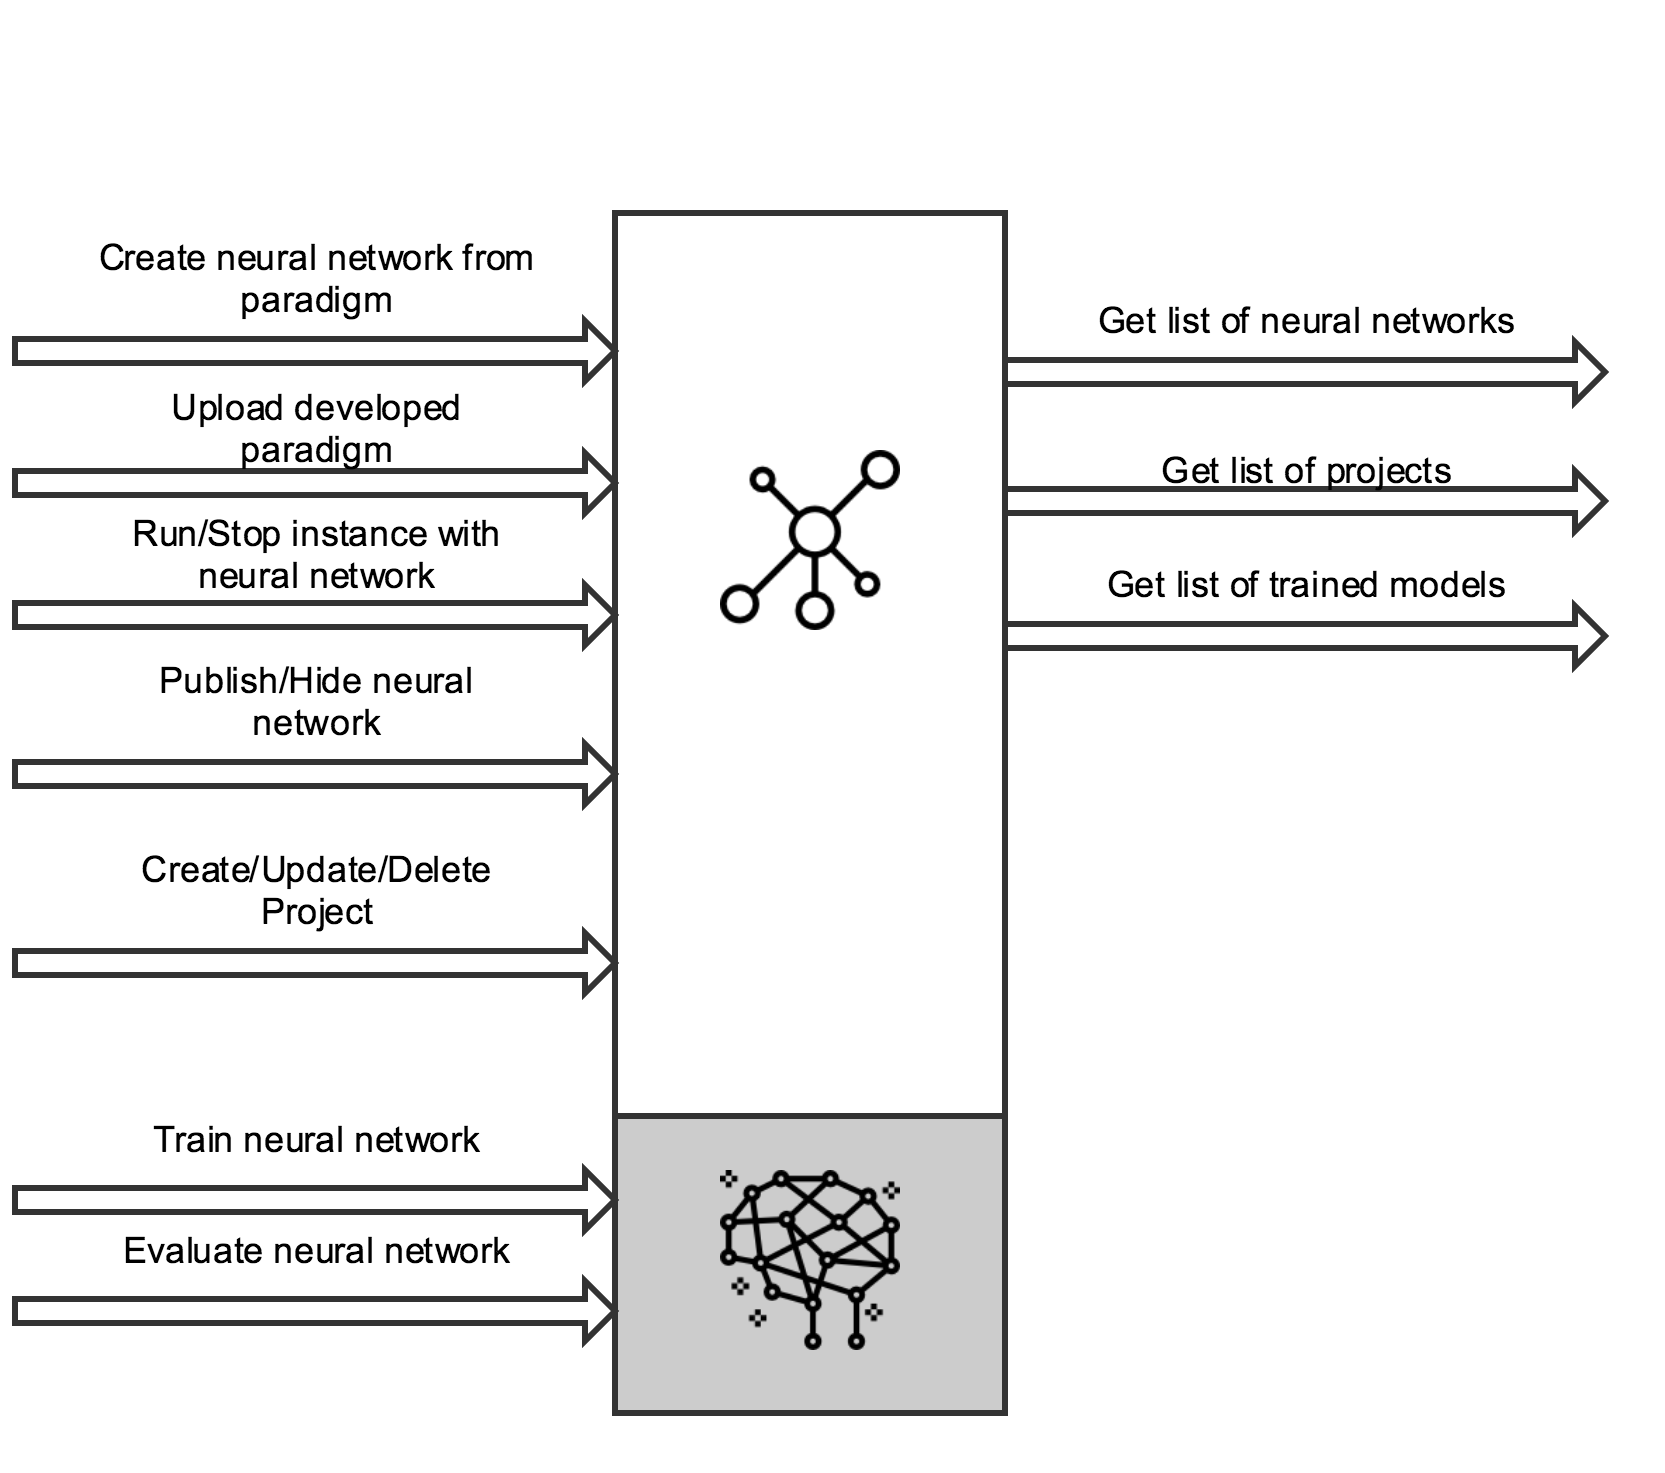
\includegraphics[width=\linewidth]{components/3/components/model_serivce.png}
  \caption{N2Sky Model Repository Web Service}
  \label{fig:model_serivce}
\end{center}
\end{figure}

As it is shown in figure \ref{fig:model_serivce} Model Repository Web Service has following accessible services:

\begin{itemize}
\item Create neural network from paradigm
\item Upload developed neural network paradigm
\item Run/Stop instance of neural network
\item Publish/Hide neural network 
\item Create/Update/Delete Project with neural networks
\item Get list of neural networks
\item Get list of projects
\item Get list of trained models 
\item Train neural network (accessible only for model management service itself)
\item Evaluate neural network (accessible only for model management service itself)
\end{itemize}

Detailed information about web service API and API documentation is written in \autoref{API Documentation}


There are two services embedded in the Model Repository web service and not exposed:

\begin{description}
\item[Training service.]  This service provides neural network training functionality. It is not possible to perform training to make the direct request on service endpoint. 

In order to perform training, the user has to know training input parameters and type of training file which can be accepted. This information is stored in ViNNSL schema. 
 
Only Model Repository web service can trigger this service after being insured that environment available and ready to perform tests. Training a is a long-term process, but it does not block an entire application. This service writes log data to the instance. Model Repository repository makes a callback to training service in order to check if training is completed. If training still processing, the Model Repository Service will fetch the log data in order to present current training result. The user can also decide to stop training process if he is satisfied with the current result.

If the user performs training on his own neural network he can also log result about his network and environment behavior. 
\item[Testing service.] The testing service allows users to evaluate a trained model.  Testing data is described in ViNNSL format. Normally testing is not a long-term process because it is running against trained neural network model. Since there is absolute freedom by neural network structure customization, the testing process can be inefficient and could take some resources from the environment. Considering this face it was decided to encapsulate this process too. 
\end{description}

\subsubsection{Cloud Management Web Service.}\label{Cloud management Web Service}  Cloud web service is originally available only for the system administrator. This service can manage OpenStack environment and Cloudify container management system. On every OpenStack instance as we as on OpenStack itself the monitoring management system service is installed. Every monitoring management system has its own metrics configurations and alerting rules. The monitoring service is only exposed via Cloud management web service. 
 
 Cloud management service supports Platform as a Service distribution. The system administrator can configure the service according to his needs. All rules, including configuration rules for monitoring and alert management systems, can be adjusted on demand.  
 
 
\begin{figure}[htbp]
\begin{center}
  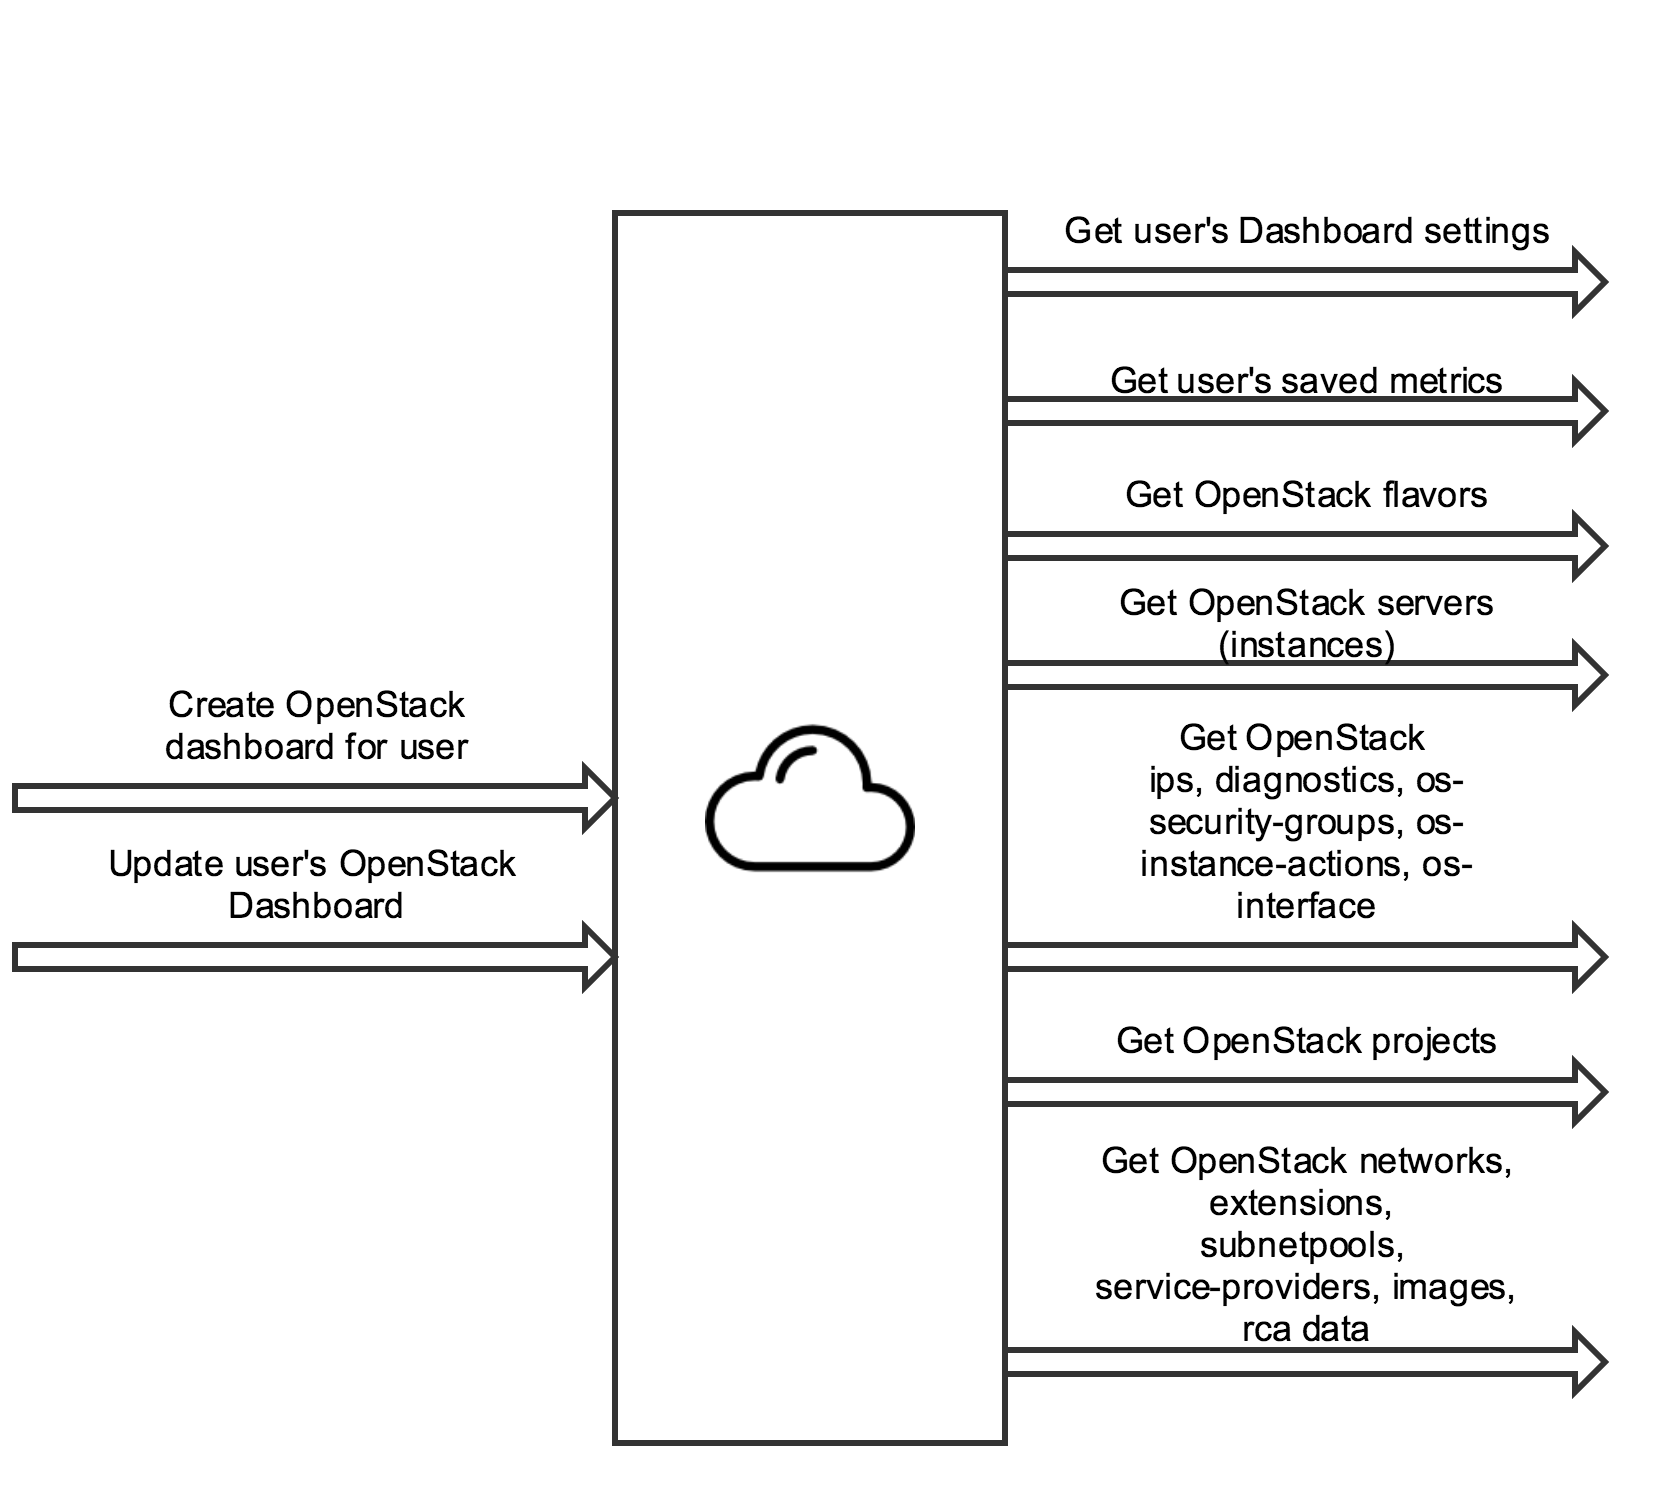
\includegraphics[width=\linewidth]{components/3/components/cloud_service.png}
  \caption{N2Sky Cloud Management Web Service}
  \label{fig:cloud_service}
\end{center}
\end{figure}

 
 As it is shown in figure \ref{fig:cloud_service} Cloud Management Web Service has following accessible services:

\begin{itemize}
\item Get user's Dashboard settings
\item Get user's saved metrics (reference to \autoref{Continuous Monitoring System} )
\item Get OpenStack Services: flavours, servers, networks, images etc.
\item Create / Update user's OpenStack Dashboard settings
\end{itemize}

Detailed information about web service API and API documentation is written in \autoref{API Documentation}


\subsection{Continuous Monitoring System}\label{Continuous Monitoring System}

In client-server architecture especially for OpenStack cloud platform, computer servers are important. Servers could go down, but the system-administrator does not have to work 24/7 in order to monitor the system and wait until some problem occurs. A system administrator could use some monitoring tools like Nagios for OpenStack in order to get information about servers state. Monitoring tool can give information about the system, network, and infrastructure \cite{nagios}. The purpose of the monitoring tool to find some problems and inform the system administrator about some problem occurred. This tool cannot solve the problem, but it can give information what went wrong.
 
\subsubsection{Monitoring requirements}\label{Monitoring requirements}

The base monitoring system is a readable and understandable representation of the graph. Graphs allow you to see objects beaning monitored and recognize metric from these objects. 
The good monitoring graph gives the meaningful description, helps quickly to detect and determine issues via representation. This kind of graph should serve as a motivation for action to solve problems. 
There are some simple rules, which makes graphing well:

\begin{description}
\item[Consistency.] Representation should correctly reflect reality. All objects, which are represented on the graph, must be correlated with a real data on the machine. 
\item[Graphs need to make sense.]  All lines represented on the chart have to be readable and understandable.  Fake or unreadable information could cause problems. Metrics set should be small, one metric represent one object. There is no need to put multiple objects which do not bind directly to one chart.
\item[Stacked area vs. multiline area.] Not every chart should have the same visual representation of the lines. Depending on the case we can decide which type of area to use.  If there are small time series with a high frequency it is better to use multiline area and stacked area on longer time series but with a bigger metric set respectively. 
\item[Understanding graph before starting to analyze it. ] Since there are going to be multiple charts with a different metrics we need to make sure that every user can understand the meaning of the particular graph. Good naming fulfilled contend and correct positioning is very important.
\item[Data hierarchy. ] It is important to define groups, metrics, data points and nested levels on the chart.  Groups help to bind similar objects together. Data points give information of time stamps. Metrics is actual graph representation. The nested level is multiple line metrics. All mentioned data should be visible and accessible. 
\item[Clarity.] Designing a chart it is important to take into consideration that there are multiple devices with a different screen resolution. Too many lines on limited space will make chart unreadable.  If there are lots of charts on one page it makes people confused what a meaning of this page. That is why it is a good practice to create multiple pages with grouped charts. 
\item[Perspective.] It is important to put graphs in such perspective so that any deviation will be easily noticeable. 
\item[Appeal.] All charts are people-oriented, people today like a simple and clean appearance of the applications and if an application has lots of charts they need to be with an appropriate design.  
\item[Control and managing.] It should be possible for any user to manipulate a graph. Either to change time series or remove some metric, customization of the graph makes the whole application more attractive.
\end{description}

\subsubsection{Applying Monitoring}\label{Applying Monitoring}
To build continues monitoring system there is a need to use a toolkit with an active ecosystem.  Searching for a proper toolkit the toolkit should be fulfilled some specific requirements that going to be used in N2Sky:
\begin{itemize}
\item Proper and self-describable metric name with a key pairs
\item Possibility to query metrics and join them in one graph.
\item Not resource-intensive
\item Support HTTP/HTTPS protocol
\item Collect and push to repository time series
\item Scalable
\end{itemize}

After researching it was decided to go for Prometheus Monitoring Toolkit \cite{alert_overview}. This tool support all requested requirements. One of the most interesting features is that Prometheus can be used on any UNIX environment. Since in OpenStack multiple instances with a different operating system can be created, Prometheus will match exact our needs. 
Originally Prometheus was created by SoundCloud team in 2012. The core of monitoring application is Prometheus server, which collects time series data from the moment it was executed on the environment as it is shown in figure \ref{fig:prometherus_arch}. All components are written in Go language and support multiple modules for monitoring different environment metrics. 
To understand the nature of Prometheus it is necessary to explain its architecture. 

\begin{figure}[htbp]
\begin{center}
  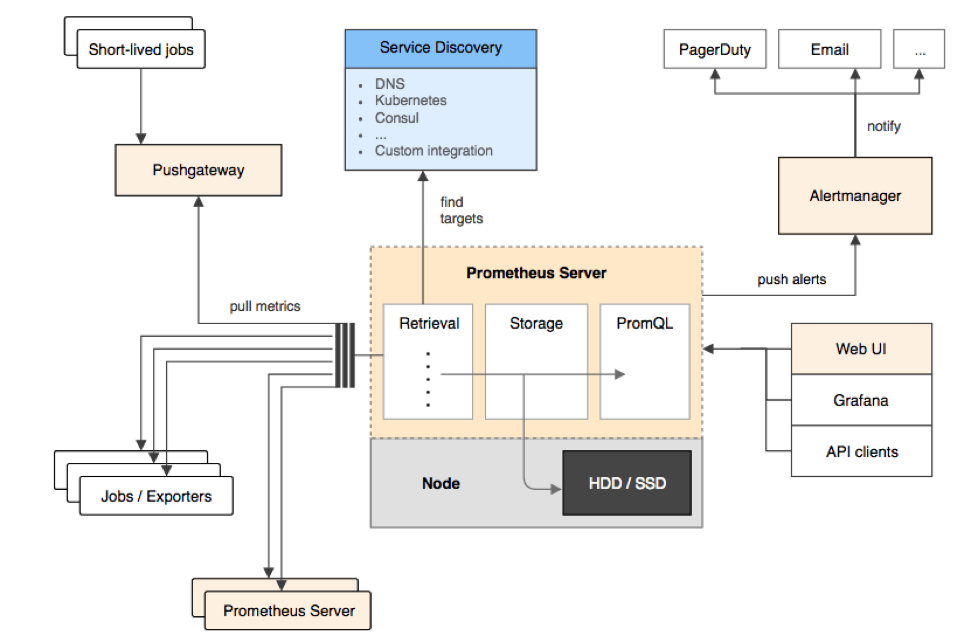
\includegraphics[width=\linewidth]{components/3/prometherus_arch.png}
  \caption{Prometheus monitoring architecture}
  \label{fig:prometherus_arch}
\end{center}
\end{figure}

The core Prometheus server pulls all metrics from jobs which are instrumented if the service is unavailable for instrumentation it can be pulled from push gateway. All metrics and logs data is stored locally so there is no distributed storage. It is possible to query this data to retrieve more specific information about particular metrics of joint metrics. N2Sky uses Prometheus API to build own customized dashboards. 
The common components of Prometheus architecture:
\begin{description}
\item[The Prometheus server.] This is the base element in the whole architecture. The server includes services which collection, storing and retrieving nodes. The principle is scrapping or pulling. It means that the data fetched with some interval, which can be configured and stored accordantly as a time series. Prometheus support different modules, each module represents some node. The nodes expose these ports that Prometheus uses for retrieving the data. For example, in N2Sky we are using Node Exporter Module which gives the possibility to collect almost all essential data like CPU, RAM, HDD/SSD etc.
\item[Push gateway.] There are some nodes, which are not exposing these endpoints. In this case collection of the data throw Push gateway is possible.  Prometheus short-lived jobs are executed to capture the data and convert it to the time series that can be used by Prometheus.
\item [Alert Manager.]  Monitoring consist of multiple metrics, each metric can be analyzed. It is possible to subscribe to particular metric in order to detect metric behavior namely metric deviations. Alert Management System used for firing events, it is possible to receive alert notification over multiple channels like Emails, SMS, Push notification etc.
\end{description}

Metric notation 
Following example represent metric notation:
\begin{lstlisting}
node_filesystem_avail {method="GET", endpoint="/api/posts", status="200"}
\end{lstlisting}

The metric naming is always self-described.  Requested metric "node\_filesystem\_avail" means available free space in the filesystem.  Every operating system has a different metric naming. N2Sky will propose the list of available metrics. In curly brackets defined the type of request, an endpoint and expected HTTP response status.

After executing this query the data will be retrieved from logs and represent as a time series as it is shown in figure \ref{fig:monitoring_req}.



\begin{figure}[htbp]
\begin{center}
  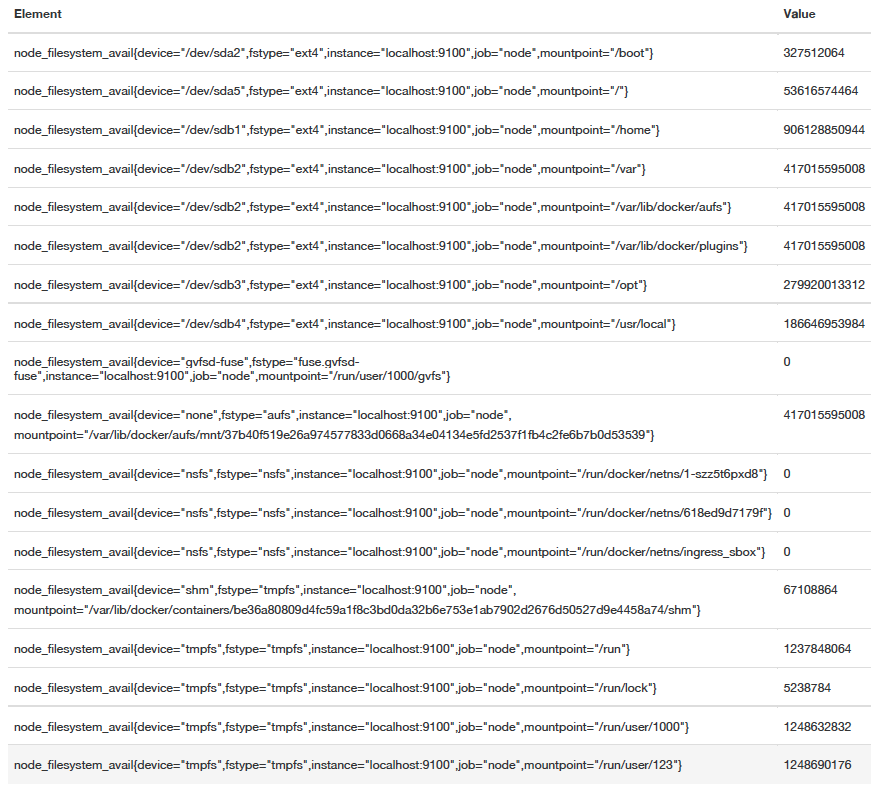
\includegraphics[width=\linewidth]{components/3/monitoring_req.png}
  \caption{Metric response}
  \label{fig:monitoring_req}
\end{center}
\end{figure}

One of the requirements of our monitoring system is scalability. One of the greatest features of Prometheus is that event if environment going to be overloaded it will generate the same amount of metrics anyway. Hence the amount of events is independent of the amount of generated time series. 
Talking about requirements it is important to mention here that there is a possibility to build joint metrics namely build multiple time series using this kind of metric:

\begin{description}
\item[Counter] The counter is a metric is representing a simple numerical value which can be incremented but not inverse. One of the typical examples is a number of expectations to have occurred. 
\item[Gauge] The gauge is a metric, which also represents a simple numerical value like a counter, but it is bidirectional. It means that this value can be decremented. The common example is CPU usage, which can go up and down.
\item[Histogram] The histogram is a metric, which represents observations.  It is stored in a bucket, which can be pulled. Any bucket can be configured depending on the need. It can be the sum of values or count of events, which are observed.
\item[Summary] The summary is a metric, which is similar to histogram but it calculates configurable quantities. 
\end{description}

\subsubsection{Integration with N2Sky}\label{Integration with N2Sky}

Prometheus supports query language, which is a key feature of this tool. The Prometheus query language, or promql, is expressive. 
With Prometheus, the self-described metric name can be chosen. Prometheus converts all metric so that every human can understand what exactly particular metric means. Let's take a previous example with a metric "node\_filesystem\_avail". This metric will show the folders on root and available memory on each of it.

\begin{lstlisting}
    node_filesystem_avail 
        {device="/dev/sdb4",fstype="ext4",
        instance="localhost:9100",job="node",
        ssmountpoint="/usr/local"}
\end{lstlisting}

Following request means that on "/usr/local" 186.6 GB is available. 

There is also the possibility to check a response code, which especially useful for alerting. 

\begin{lstlisting}
        node_filesystem_avail {status="500"}
\end{lstlisting}

This request returns some response code 500 namely internal server error. 

For building a proper dashboard for monitoring it is important to provide customization that is why Prometheus supports time duration:

\begin{itemize}
\item s - seconds
\item m - minutes
\item h - hours
\item d - days
\item w - weeks
\item y - years
\end{itemize}

Using the time duration with an offset it is possible to get an exact metric on demand. 
Building query with a Prometheus can bring lots of advantages. For example, there is the query which  a counter with an available node file system metric:

\begin{lstlisting}
    took( 3, sum(
         rate(api_http_requests_total{status=500}[1h]
    ) )
     by (endpoint)
     )
\end{lstlisting}

This query is already complicated, but it can be extended by multiple new rules and constraints. 

In N2Sky was developed monitoring service, which uses microservices approach like an entire application. It was decided to get rid of complex queries and provide some intuitive way of creating metrics. 
First of all the time range add a complexity. It was decided that the user should give only time interval and step. Let's say the user wants to see CPU load for the last hour with a step 30 seconds. It makes the creation of metric more intuitive, no more range like "from", "to" and type of ranges. All this can be solved with one simple request. 
The second part is a storing of metric. Instead of every time build a query the monitoring service saving requested by user metric. In this case, every user will get his own customized metric. 
The service uses Mongo DB for storing the metric configuration. Every collection has its own schema. When a user makes a request to save a metric the schema has to be filled with a requested by user data.

\subsubsection{Monitoring dashlet Design}\label{Monitoring dashlet Design}

Since there are multiple machine and services to monitor there was a need to create a dedicated dashboard design.  At first, let's take a look at the environments we have to monitor: 
\begin{description}
\item[Openstack Machine.]  It is dedicated machine, our cloud base for development and running instances.
\item[Openstack Instances.]   Virtual machines with a different OS.
\item[Docker Containers.]  Virtual machines in the OpenStack instances.
\end{description}

One of the most important parts of application design is to maximize reusability of the components. 


The benefit of the microservices architecture is the independence of each service. The good part of it, when one of the services will not be accessible, the rest of them still be up and running. The problem is that in order to make application running correctly all services are required. It is important to detect events and rollbacks the transaction in case if the error or failure occurs. N2Sky system has its own monitoring and alerting system, which notify the system administrator about failures, but how to handle events, which are transactionally dependent from service to service in case if the error occurs and an event is still in the transaction. There is two main kind of events \cite{cs5366}: 

\begin{itemize}
\item \emph{Intrinsic Events.} Process steps starting and finishing generate events intrinsic to the process model. This kind of events contains the process step or failure. 
\item \emph{Context Events.} Events stemming from the context of the process.
\end{itemize}

It is impossible to maintain each event and process an event stream in the N2Sky application because if some other developers forget to put the event into the stream it will not be noticed. That is why in N2Sky is events intrinsic, which are logging every transaction from one service to another. In case if the error occurs the alerting event will be fired with a log data like the step it self and the error. 

 
\begin{figure}[htbp]
\begin{center}
  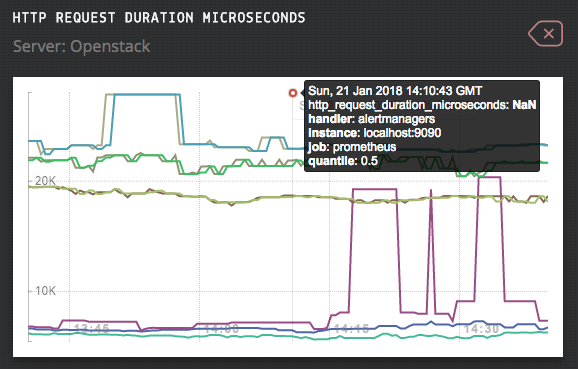
\includegraphics[scale=0.65]{components/3/components/monitoring_dashlet.png}
  \caption{N2Sky Monitoring Dashlet}
  \label{fig:monitoring_dashlet}
\end{center}
\end{figure}

 
The figure \ref{fig:monitoring_dashlet}  shows HTTP request directions in milliseconds metrics. Each dashlet item contains:
\begin{itemize}
\item Title, which represents readable and self-described metric name.
\item Server, which shows to which instance this metric belongs.
\item Chart is the monitoring data itself. 
\item Tooltip, which appears on metric mouse over. Tooltip shows following data:
\begin{itemize}
\item Date of the particular position.
\item Name of metric
\item Instance environment 
\item Handler is an alert manager listener (reference to \autoref{Alerting Management System})
\item Cron job
\item Quintile 
\end{itemize}

\end{itemize}


\subsection{Alerting Management System}\label{Alerting Management System}

Today the most trending subject in monitoring area is a prediction and automated detection. It makes people free from 24/7 managing, maintaining, and monitoring system.
For monitoring, we are using Prometheus tool. Since this tool saving constantly logs data about the system it is possible to reuse this logs to build an alert system. 
Prometheus tool provides an Alert Manager module. Natively this tool supports different notification methods like email notification or some request on Slack. 

\subsubsection{Alerting System Architecture}\label{Alerting System Architecture}

Since the Alert Manager is a part of Prometheus Tool it has its own binary. The idea behind is to have only one Alert Manager and have monitoring tool on multiple machines. If the machine goes down or even Prometheus itself, the Alert Manager can catch and deliver this event. 
To understand how Alert Manager works it is essential to understand the architecture of the whole system as it is displayed in figure \ref{fig:alert_arch}.

\begin{figure}[htbp]
\begin{center}
  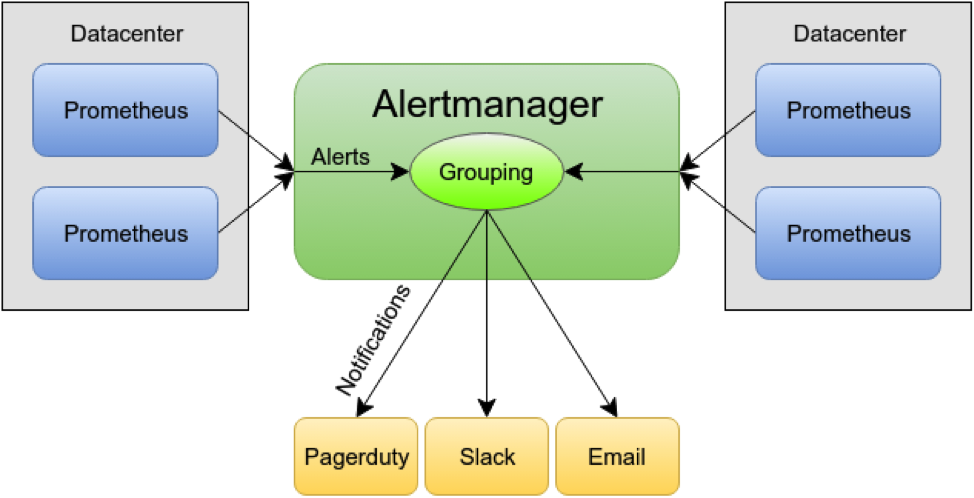
\includegraphics[scale=0.6]{components/3/alert_arch.png}
  \caption{Alerting System Architecture}
  \label{fig:alert_arch}
\end{center}
\end{figure}

This architecture is a typical messaging platform.
Messaging Service sends messages to multiple clients. It is implemented Producer-Consumer Pattern. In the Alert Manager Architecture, the role of the producer is taken by Prometheus Datacenter. Alert Manager consumes the messages. The consumer knows nothing about the producer and just subscribe to the event. With this approach, it is possible to attach multiple producers \cite{alert_book}. 

Alerts can be collected in groups by the datacenter. It means if an event occurs on multiple machines it can be packed into one notification and fired accordingly. 
In Prometheus configuration need to be set up only two things: reference on Alert Manager and Alert Rules. When Alert Manager consumes an event it just dispatches it via notification as it is displayed in figure \ref{fig:alert_arch_detailed}.

\begin{figure}[H]
\begin{center}
  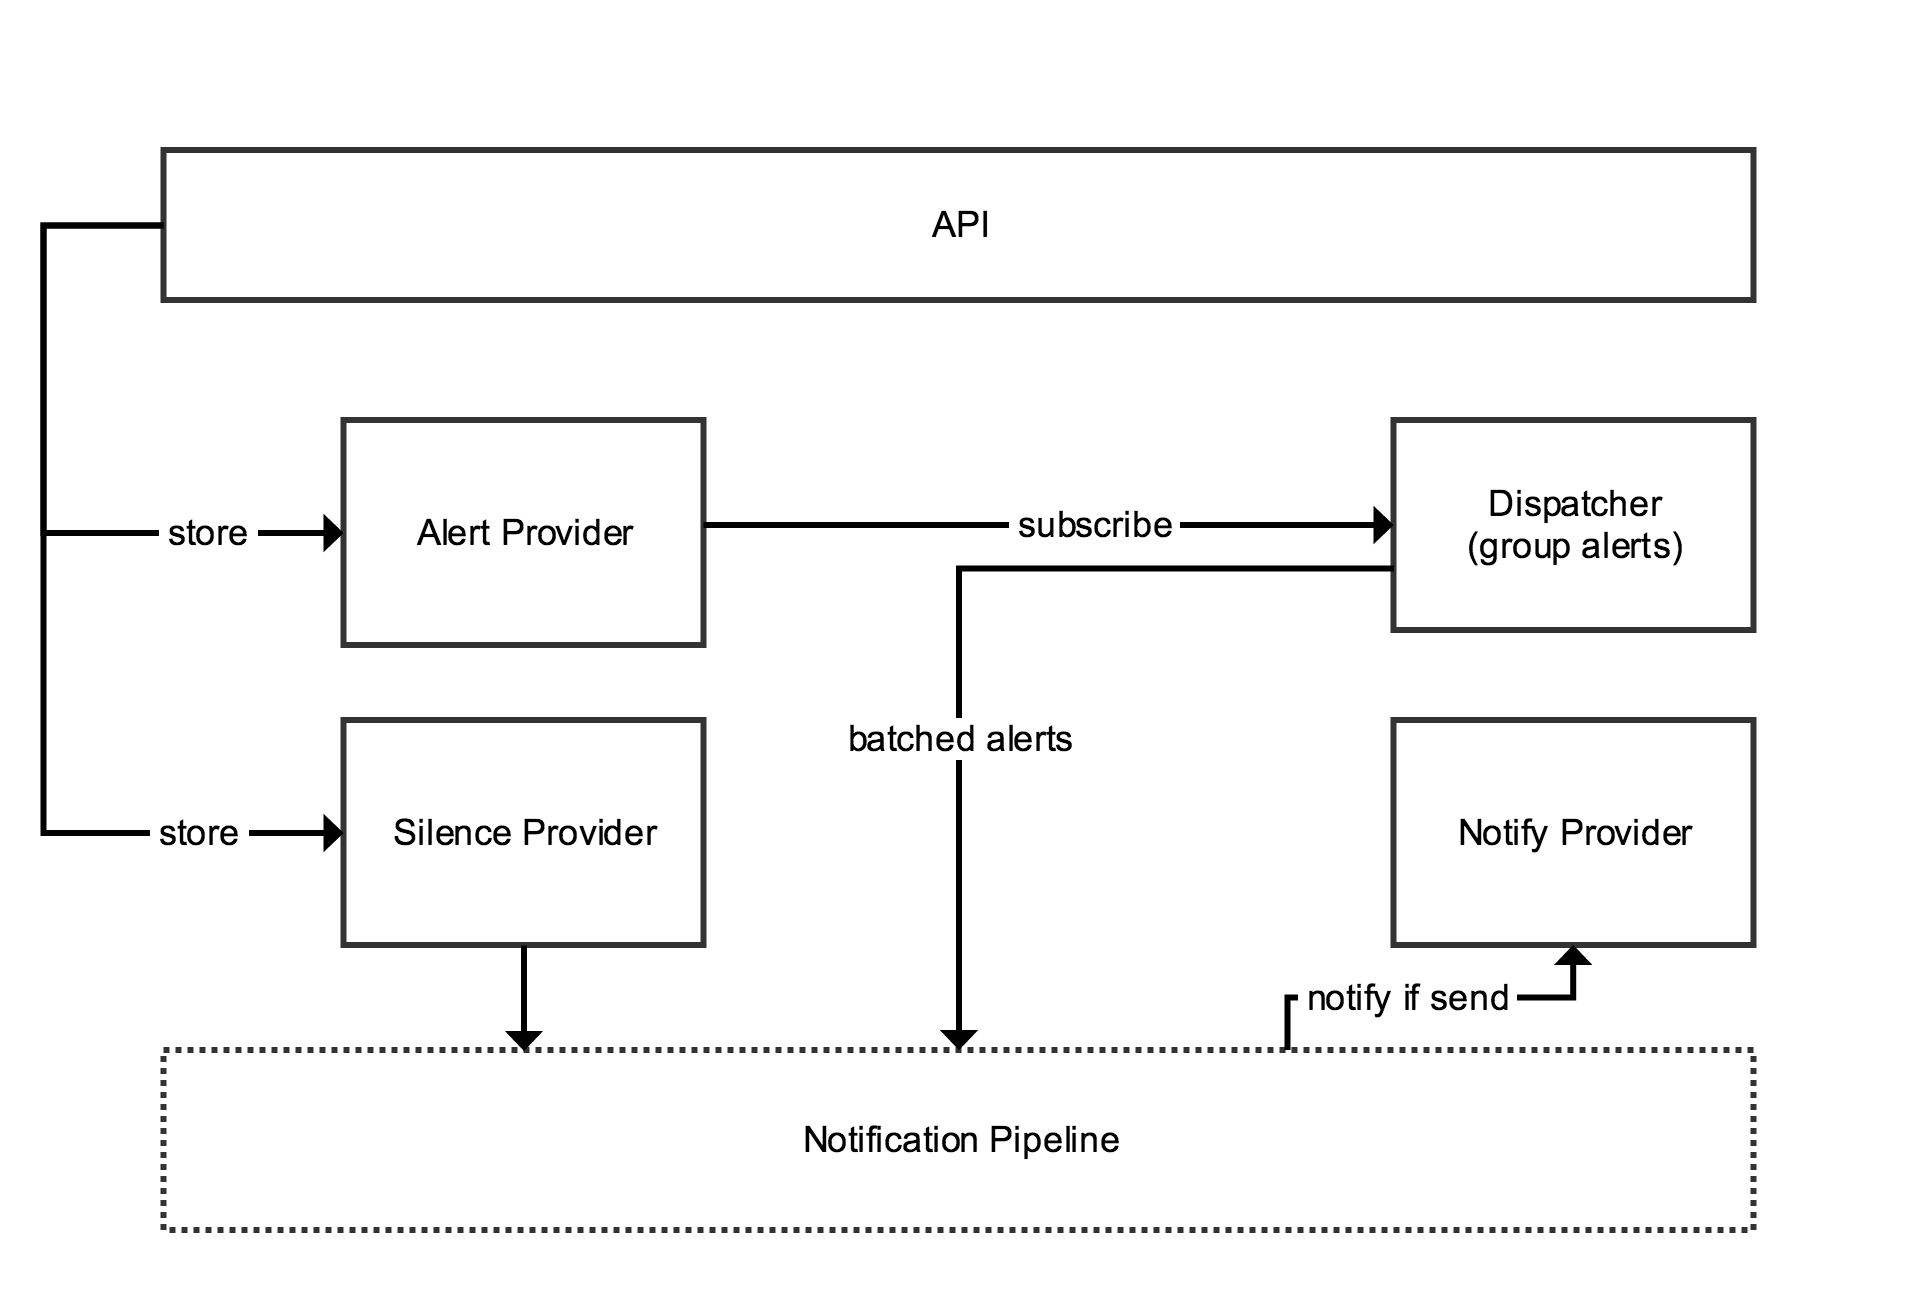
\includegraphics[width=\linewidth]{components/3/alert_details.png}
  \caption{Communication within Alerting Management System}
  \label{fig:alert_arch_detailed}
\end{center}
\end{figure}

\begin{description}
\item[API] Alert manager API has only one endpoint, which gives the list of events that occurred.
\begin{lstlisting}
            /api/v1/alerts
\end{lstlisting}

As a response the event information is sent \cite{alert_send}.
 \begin{lstlisting}
 [
  {
    "labels": {
      "<label>": "<value>"
    },
    "annotations": {
      "<label>": "<value>",
    },
    "startsAt": "<date>",
    "endsAt": "<date>"
    "generatorURL": "<url>"
  }
]
\end{lstlisting}
Following response shows timestamp of event, additional information as an annotation and name of event (alert). 
\item[Silences.] Silences is a commands, which are muting alerts for specific time. It can be configured via web interface. 
\item[Dispatcher.] Dispatcher is a grouping of alert with a similar nature into single notification. This will be send as a batch to Notification pipeline.
\item[Notification Pipeline.] Is a pipepline, which consists channel, router and filter. It takes rules from Alert Provider and Silence Provider and alerts from Dispatcher. If notification is ready it can be send. 
\end{description}


\subsubsection{Alert Rules}\label{Alert Rules}

As it was mention one of the main changes in Prometheus setup is to configure the alert rules. Every Prometheus Monitoring Tool can have it own alerting rules, which can be defined. There is also a possibility to reference on some common alerting rule for every monitoring system on every machine. 

 \begin{lstlisting}
        groups:
        - name: test
          rules:
          - alert: Error
            expr: job:request_latency_seconds:mean5m
            {job="loclhost:5000"} > 0.5
            for: 5m
            labels:
              severity: page
            annotations:
              summary: latency
\end{lstlisting}

Following the example of alerting rules shows the typical alerting rule. Most important parts are an expression, which is applied to Monitoring System and severity level.  More details about the creation of alerting rules are located in Development Guide chapter "Setting up Alert Management System" \autoref{Setting up Alert Management System}.

Alerting rules are instructions to the monitoring system it can be useful as well for alerting as for recording. 

Recording rules allow to pre-compute frequently needed expressions or expressions, which are resource or time-consuming.  These rules are saving the result in a new set of time series. It is like indexing this data, so that prevent expansive I/O methods. 
The rules are being executed sequentially with a predefined interval. 
With an alerting rule, it is possible to define alert namely deviation by particular expression from Prometheus Tool and its exports (modules). It allows building an alert even on the combined query. 

In case if Alert Manager is not available all alerts are saving into the buffer. As soon Alert Manager online all events will be fired sequentially. 



\subsubsection{Integration with N2Sky}\label{Integration with N2Sky Alerting}

Alerting System is represented as a module in N2Sky. 
Alerting Client is the additional configuration of Prometheus Monitoring System. When Prometheus will be executed it should have the reference to Alerting System and its rules. 
Since the client should be installed on each OpenStack instance it was integrated into image snapshot. When the new instance will be spawned with an OpenStack snapshot, the client will be automatically executed there.  

Alerting Client fire alerts depending on configured rules. The rules can be created via the user interface. The list of events N2Sky receives via its service, which fetches information from Alert System. 
 
\subsubsection{Alerting System Design}\label{Alerting System Design}

Developing Alerting System UI it kept the same design as in entire application. The N2Sky UI components were reused and none of the new components were created. The main component is a grid item which contains information about event, which is occurred  as it is shown in figure \ref{fig:alert_grid}.

\begin{figure}[htbp]
\begin{center}
  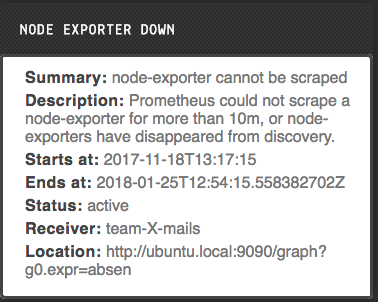
\includegraphics[scale=0.7]{components/3/alerts/alert_grid.png}
  \caption{N2Sky Alerting Management System Event representation.}
  \label{fig:alert_grid}
\end{center}
\end{figure}

The following information is shown:

\begin{description}
\item[Title.] The name of alert.
\item[Summary.]   Short is a description of the alert. If the summary is too long it will be cut.
\item[Description.] The whole description of the alert.
\item[Starts at.] Timestamp when the event occurred. 
\item[Ends at.] Timestamp when the event is no more valid. If the timestamp is a current day and time, the problem still not fixed. 
\item[Status.] Actual status of the event. Can be active and inactive.
\item[Receiver.] The group of receivers. Normally group contains multiple receivers emails. 
\item[Location.] The endpoint of the server where monitoring system installed. 
\end{description}

Every alert has its severity level. Depending on it the fired events will be represented differently. Every severity level has own color on N2Sky as it shown in ``Fig.~\ref{fig:alert_severity}''.

\begin{figure}[htbp]
\begin{center}
  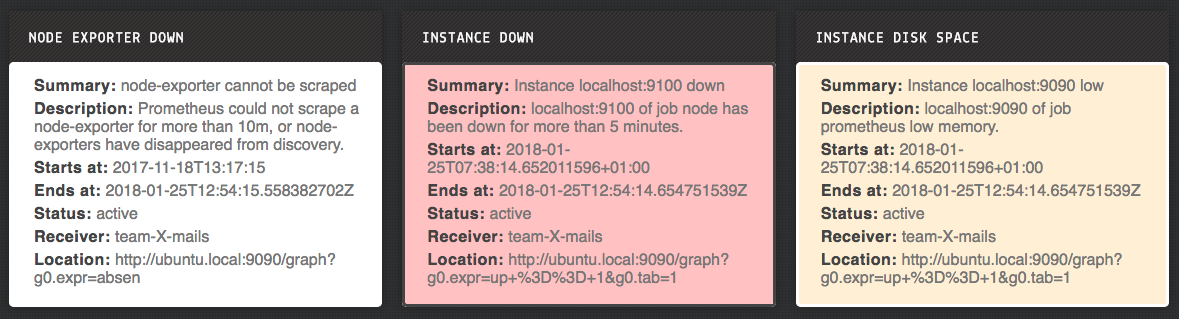
\includegraphics[width=\linewidth]{components/3/alerts/alert_severity.png}
  \caption{N2Sky Alerting Management System Severity Level}
  \label{fig:alert_severity}
\end{center}
\end{figure}

There are three types of severity levels:
\begin{itemize}
\item Critical, which shows that crucial event occurs. For example, if the server goes down it is critical severity level.  In N2Sky UI it has a red color. 
\item Warning, which shows that something goes wrong. For example not enough disk space on the server. In N2Sky UI it has the orange color. 
\item Page, which shows that some information. For example, lots of requests occurred. In N2Sky UI it has the white color.  
\end{itemize}
 




\section{Vienna Neural Network Specification Language}\label{ViNNSL 2.0 extended}

In this chapter will be described the history if the ViNNSL language, its development, and new features, which are applied in the current N2Sky system.

\subsection{ViNNSL Development}\label{ViNNSL Development}
Vienna Neural Network Specification Language (ViNNSL) is the language, which used for a description of the semantic and behavior of the neural network paradigm. ViNNSL gives a possibility to create dynamic services, which can differentiate the behavior. The ViNNSL have been seen as a semantic language standard. The language uses schemas, which helps users to describe attributes like service capabilities, semantic, functions, and parameters \cite{Beran2008}.

ViNNSL consist of five parts:
\begin{itemize}
\item Description Schema
\item Definition Schema
\item Data Schema
\item Result Schema
\end{itemize}

This approach with multiple schemas was used in Neural Network Cube (N2Grid) System. This system is a web-based neural network simulator used by students and researchers \cite{schikuta2004n2grid}. Today N2Sky is the follower of the N2Grid ideas. 

In 2015 the ViNNSL 2.0 was released, which was the extension of the previous version \cite{ijcnn15}. Basically, almost nothing changed only additional fields were added:
\begin{itemize}
\item \emph{Creator}
\item \emph{Problem Domain}
\item \emph{Propagation Type}
\item \emph{Learning Type}
\item \emph{Application Field}
\item \emph{Network Type}
\item \emph{Problem Type}
\item \emph{Execution Environment} The idea was proposed back then by the concept of the N2Grid \cite{schikuta2004n2grid}. It is possible to define the environment, which is needed for particular neural network instance. 
\item \emph{Execution Type.} It became possible to define how neural network will be executed either sequential or parallel. In detailed, it was possible to define perform processing and the type of the architecture.
\item \emph{Result Schema} became a part of the ViNNSL Description. Earlier it was separated schema, but data schema and instance schema still remain the same.
\item \emph{Parameters} The user could define input as well as output parameters. It was possible to define also file for neural network training.
\end{itemize}

\subsection{ViNNSL Template}\label{ViNNSL Template}

After studying ViNNSL with its extension it was decided to simplify the whole schemas and most importantly adapt it to the current N2Sky system.

The idea behind to use the ViNNSL template, which has additional fields for ViNNSL 2.0, but they can be fully processed and taking away after creating the neural network. No more extra objects or fields in other application. ViNNSL template allows the user to apply the ViNNSL language across the whole N2Sky platform. The detailed information is shown in \autoref{A}

\subsubsection{Metadata template}\label{Metadata template}

As it was mentioned before, the ViNNSL 2.0 contains metadata about the user and neural network.

\begin{lstlisting}[caption=ViNNSL template metadata]
...
	"problemDomain": {
		"propagationType": {
			"value": null,
			"possibleValues": ["feedforward"],
			"learningType": {
				"value": null,
				"possibleValues": ["definedconstructed", 
				"trained", "supervised", "usupervised", "linear"]
			}
		},
		"applicationField": {
			"value": null,
			"possibleValues": ["AccFin", "HealthMed", "Marketing",
			 "Retail", "Insur", "Telecom", "Operations", "EMS"]
		},
		"problemType": {
			"value": null,
			"possibleValues": ["Classifiers", "Approximators",
			 "Memory", "Optimisation", "Clustering"]
		},
		"networkType": "Backpropagation"
	}
...
\end{lstlisting}

From code above it is possible to spot some additional values:
\begin{itemize}
\item \emph{value} is the default value of the object. 
\item \emph{possibleValues} parameter, which contains the array of possible value. The user can choose one of the value. 
\end{itemize}

This approach not only helps to add templating into the current ViNNSL schema but also add some rules upon it:
\begin{itemize}
\item If default value set and there are no more values under "possibleValues" parameter, then the value is impossible to change.
\item If there is no value for "possibleValues" and "value" fields than the user can type customized value.
\item If the "value" has some parameter and "possibleValues" field is also not empty it means that the "value" parameter is the default value and it can be changed by "possibleValues".
\end{itemize}

\subsubsection{Environment}\label{Environment}

In previous versions of the ViNNSL language, it was possible to define execution environment. This possibility is still available, but some additional value was added in order to apply templates. 

In the current version of N2Sky, it is possible to deploy neural network on the N2Sky cloud as well as on private cloud of the user. That is was the "endpoints" parameter was added.

\begin{lstlisting}[caption=ViNNSL template enviroment]
...
    "endpoints": [{
        "name": "train",
        "endpoint": null
    }, {
        "name": "test",
        "endpoint": null
    }]
...
\end{lstlisting}

Since it is array parameter it gives room for adding new endpoints in case if it will be needed in future versions of the N2Sky.

\subsubsection{Neural Network Structure Template}\label{Neural Network Structure Template}

The structure of the neural network was also changed. The template looks pretty empty, but from this template is possible to generate any type of structure based on ViNNSL language. 

\begin{lstlisting}[caption=ViNNSL template structure]
...
"structure": {
		"inputLayer": {
			"result": {
				"nodesId": []
			},
			"config": {
				"dimensions": {
					"min": 1,
					"max": 1
				},
				"size": {
					"min": 960,
					"max": 960
				}
			}
		},
		"hiddenLayer": {
			"result": {
				"dimensions": [{
					"id": null,
					"nodesId": []
				}]
			},
			"config": {
				"dimensions": {
					"min": 1,
					"max": 1
				},
				"size": {
					"min": 960,
					"max": 960
				}
			}
		},
		"outputLayer": {
			"result": {
				"nodesId": []
			},
			"config": {
				"dimensions": {
					"min": 1,
					"max": 1
				},
				"size": {
					"min": 960,
					"max": 960
				}
			}
		},
...
\end{lstlisting}

The structure contains input, hidden and the output layer. Hidden layer has "dimensions" parameter, which allows creating multiple hidden layers.

 Every layer has "config" property, which shows how many dimensions is possible to use. This config is scalable, it is possible to add additional configuration or use none of them.
 
 Additionally, every layer has a number of nodes, namely the neutrons id.  
 
 In structure is important to define the connections between nodes. 
 

 \begin{lstlisting}[caption=ViNNSL template connections]
...
		"connections": {
			"fullyConnected": {
				"isConnected": null
			},
			"shortcuts": {
				"isConnected": null,
				"connections": [{
					"from": null,
					"to": null,
					"isFullConnected": null
				}]
			}
		}
	}
...
\end{lstlisting}

There are few types of connections:
\begin{itemize}
\item \emph{fullyConnected} parameter, which has boolean "isConnected" in case if the neural network fully connected or not.
\item \emph{shortcuts} is a parameter, which also has boolean flag parameter. If there are any types of the shortcuts is will be set to true. Inside of this parameter is an array field "connections". This array has from and to node id parameter and in case if the full connection remains the same this "isFullConnected" will set on true.
\end{itemize}

\subsubsection{Parameters Template}\label{Parameters Template}

To the input parameters, the templating was also applied. The structure of the template is pretty similar to metadata template.

 \begin{lstlisting}[caption=ViNNSL template input paramteres]
...
"parameters": {
		"input": [
			{
				"parameter": "activationFunction",
				"defaultValue": "sigmoid",
				"possibleValues": ["sigmoid", "relu", "softmax"]
			},
			{
				"parameter": "activationFunctionHidden",
				"defaultValue": "relu",
				"possibleValues": ["sigmoid", "relu"]
			},
...
\end{lstlisting}

Additionally in this template used the "parameter" field. This field defines actual input parameter and has to be unique.

The output parameter is fixed and can not be changed. This parameter will be used for trained model evaluation in case if the user does not want to type own testing data.

The training file information also defined under parameters and can be changed only by neural network owner.


\subsection{ViNNSL Generation}\label{ViNNSL Generation}

After the neural network contributor user fills out the template ViNNSL it is possible to generate the ViNNSL Description schema. This schema will be used for neural network training. The generation is happening  on the N2Sky platform and the ViNNSL Description file can be totally different, but the rules will be followed. The user now has a possibility to customize the structure, connection, metadata and parameters of the neural network. It is impossible to do something wrong because permissions are restricted by ViNNSL Template. 

The contributor user can also user ViNNSL in order to fill out the structure, connection, metadata and parameters of the neural network. If the user manually will do it, without N2Sky "3-step-view" generator, he has to upload his ViNNSL in the N2Sky platform and the neural network will be automatically created. 

\subsubsection{Generated Metadata}\label{Generated metadata}

In generated metadata, the information is filled out from N2Sky platform.

All unless fields will be removed automatically, even if the contributor user leave it there. The typical parameters like "possibleValues" will be removed everywhere except the training parameters because it is needed for performing training.

 \begin{lstlisting}[caption=Generated ViNNSL model]
 ...
	"problemDomain": {
		"problemType": "Classifiers",
		"networkType": "Backpropagation",
		"applicationField": [
			"AccFin"
		],
		"propagationType": {
			"propType": "feedforward",
			"learningType": "supervised"
		}
	},
	"creator": {
		"name": "fedorenko",
		"contact": "andriifedorenko@gmail.com"
	},
	"metadata": {
		"name": "XOR Test",
		"description": "test",
		"paradigm": "Backpropagation",
...
\end{lstlisting}

The detailed information is shown in \autoref{B}

\subsubsection{Generated Structure}\label{Generated structure}

The structure is the most complicated part of the ViNNSL generation if the user will do it manually without N2Sky generator. 

Every node will receive the id, which will be parsed by N2Sky.

\begin{itemize}
\item \emph{Input layer as well as output layer} has the same structure of the node ids.
 \begin{lstlisting}[caption=ViNNSL generated layers]
...
		"inputLayer": {
			"amount": 3,
			"nodesId": [
				"1-input",
				"2-input",
				"3-input"
			]
		},
		"outputLayer": {
			"amount": 1,
			"nodesId": [
				"1-output"
			]
		},
...
\end{lstlisting}

Every node has the amount of the nodes. The nodes id have the following structure: 
\begin{enumerate}
\item The unique id of the node, which also defines the order
\item The name of the layer
\end{enumerate}
\item \emph{The hidden layer} can be multidimensional, that is why the id of the layer, as well as the id of nodes, are required.


 \begin{lstlisting}[caption=ViNNSL generated hidden layers]
...
		"hiddenLayer": [
			{
				"id": "1-hidden-layer",
				"amount": 4,
				"nodesId": [
					"1-node-1-hidden-layer",
					"2-node-1-hidden-layer",
					"3-node-1-hidden-layer",
					"4-node-1-hidden-layer"
				]
			},
...
\end{lstlisting}

The id of the layer dined by the first number, which is also the order of the layer.

The id of the nodes defined by following rules:
\begin{enumerate}
\item The unique id of the node, which also defines the order
\item The id of the layer
\item The name of the layer
\end{enumerate}

\end{itemize}


\subsection{ViNNSL Model}\label{ViNNSL Model}

The ViNNSL Model is a derived from ViNNL Description trained model. Basically, the input parameters were taken from the ViNNSL Description and default values were replaced with the trained data. Additionally, it was decided to put following parameters:

\begin{itemize}
\item \emph{rawModel} is the raw training model, which can be used for the model evaluation. 
\item \emph{logs.} The logs are appending during the training. When the training has done the logs will be removed from the neural network and added as a parameter to the model.
\item \emph{test} is the array of performed tests. It was decided to save the test results in the model in order to stop spreading multiple schemas. 
 \begin{lstlisting}[caption=ViNNSL trained model testing]
...
       {
                "createdOn": "2018-02-24T12:24:38.198Z",
                "result": "[[0.]\n [1.]\n [1.]\n [1.]]",
                "testing_data": "[[0,0],[0,1],[1,0],[1,1]]",
                "user": "admin"
            }
 ...
\end{lstlisting}
The test has following data:
\begin{itemize}
\item \emph{createdOn} timestamp of the testing
\item \emph{testing\_data} with which the model was tested
\item \emph{result} actual result of the testing
\item \emph{user} the user, who performed test.
\end{itemize}
\item \emph{paramters} the input parameters, where default values were replaced with the actual values. 
\end{itemize}

Detailed example of the ViNNSL model is located in \autoref{C}

\section{Functional requirements specification}\label{Functional requirements specification}

\subsection{User Roles}\label{User Roles}

In order to make the N2Sky user interface understandable for arbitrary users as well as professional for advances users, it was decided to separate the user roles. Every user role has own way of interaction with the application:

Every user has some specific area within he works. For example just registered user does not need to know the current environment monitoring information. These restrictions were motivation to create some user roles in order to restrict of grand some functionality of N2Sky.

\begin{itemize}
\item The contributor is an arbitrary user. Such a user has no necessity in having deep knowledge of the neural network field or know any programming language. The main goal of arbitrary user is to study neural networks within N2Sky. The contributor has an access only to his own dashboard and public available resources on the main application module. He can perform semantic search for available neural network paradigms and use them. He can also train running neural network instances and test them. This user can share his trained neural network by making it public. 
\item The developer is an expert user, which has enough knowledge and experience to create his own neural network. This user can create neural network paradigms using the ViNNSL schema and publish them on N2Sky. This user can deploy neural networks on the N2Sky environment as well as on his own environment by providing training and testing endpoints. The goal of the developer is the study how his networks will behave with different network structures, input parameters and training data that is provided by other users.
\item System administrator is a user who has a full access to application including environment management, monitoring and alerting features. Administrator can manage Openstack and Cloudify instances. He also can shadow any N2Sky user to observe the application from shadowed user perspective. Administrator has access to all dashboards in every module.
\end{itemize}


\subsection{Administration components}\label{Administration components}
\subsubsection{Affected users}\label{Affected users}
\subsubsection{Administration Dashboard}\label{Administration Dashboard}
\subsubsection{Openstack Dashboard}\label{Openstack Dashboard}
\subsubsection{Cloudify Dashboard}\label{Cloudify Dashboard}
\subsubsection{Alerting System}\label{Alerting System}
\subsubsection{Monitoring System}\label{Monitoring System}

\subsection{N2Sky Components}\label{N2Sky Components}
\subsubsection{Affected user groups}\label{Affected user groups 2}
\subsubsection{N2Sky Dashboar}\label{N2Sky Dashboar}
\subsubsection{Neural Networks Repository}\label{Neural Networks Repository}
\subsubsection{Models Repository}\label{Models Repository}


\section{Requirements specification for Main Application Module}\label{Requirements specifications for Main Application Module}
\subsection{General Definition}\label{GeneralDefinition main}
Main Application Module (MAM) is an application, which responsible for management N2Sky system. It embeds:
\begin{itemize}
\item Model Repository 
\item Neural Network Repository 
\item N2Sky Main Dashboard.
\end{itemize}

MAM is a core component of the N2Sky platform. From this component, users can feel the power of the N2Sky system and try out the whole functionality of it. The MAM, as well as other N2Sky components, is possible to use on any device because it supports responsive design. 

\subsection{Affected Users}\label{Affected users MAM}
The MAM has one User Interface but users can use it diverse. Only users, which the main function is within MAM can operate this module on their own purpose. Following types of users have this kind of the main function:

\begin{itemize}
\item \emph{Arbitrary User.} The main function of the arbitrary user is to learn about neural networks or try out his knowledge in this field. The typical use case is when the user logs in from the mobile device like smartphone all tablet and search something in repositories. This user copy existing neural networks or trained models into own project and perform some operations on it.  A detailed description is in \autoref{User Roles}. 
\item \emph{Neural Network Engineer User.} This kind of user normally uses Desktop version of N2Sky, but he can also use the mobile version because all functionalities are also available there. The user creates own neural network from existing paradigm, but he also can act as an Arbitrary User.  A detailed description is in \autoref{User Roles}. 
\item \emph{Contributor User.} The Contributor uses N2Sky MAM component mostly for an easier way to check his own neural network paradigm. Since this user can fully use N2Sky open API, UI for him is just for the quick check. The UI is available also in the mobile version, that is why Contributor can observe his neural networks behavior directly from the mobile device in any place. A detailed description is in \autoref{User Roles}. 
\item \emph{System Administrator.} His main function is on AM module, but since he is also the administrator of the N2Sky MAM he can see all processes of other users. This user can shadow any other user in order to see what is happening in particular user dashboard.  A detailed description is in \autoref{User Roles}. 
\end{itemize}

\subsection{N2Sky Dashboard}\label{N2Sky Dashboard}
The N2Sky dashboard is the central component of the MAM module. The dashboard gives brief information about available tools, user's projects and user's neural networks. Every dashboard is unique for every user, namely, the content always differs. As it is displayed in figure \ref{fig:n2skymaindashboard}, the dashboard gives a full overview of the components from one page.

\begin{figure}[H]
\begin{center}
  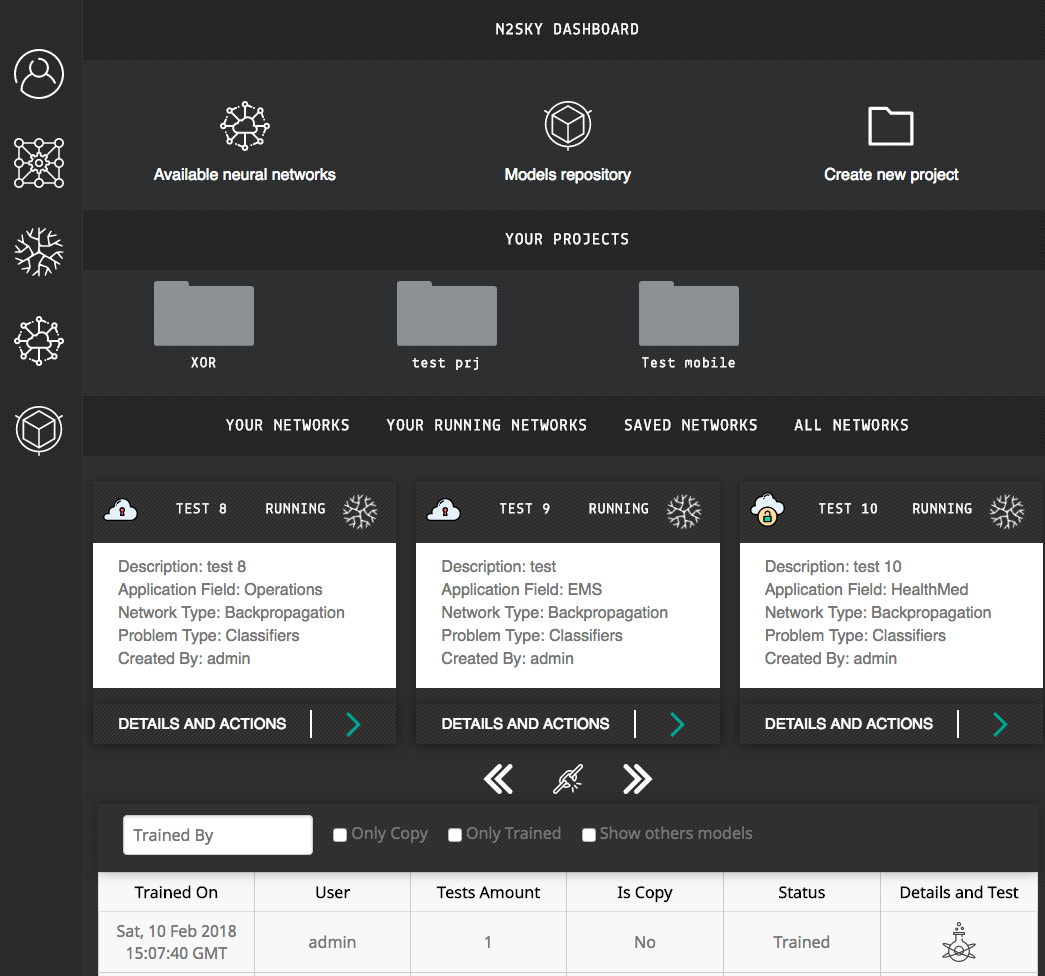
\includegraphics[width=\linewidth]{components/5/img/n2sky_main_dashboard.png}
  \caption{N2Sky User Dashboard}
  \label{fig:n2skymaindashboard}
\end{center}
\end{figure}

The N2Sky dashboard contains following components:
\begin{itemize}
\item Available tools
\item The user projects
\item The user neural networks 
\item The user trained models
\end{itemize}

The dashboard is available under following URL path:
 \begin{lstlisting}
    <host>/cloud
\end{lstlisting}

\subsubsection{Available Tools}

\begin{figure}[htbp]
\begin{center}
  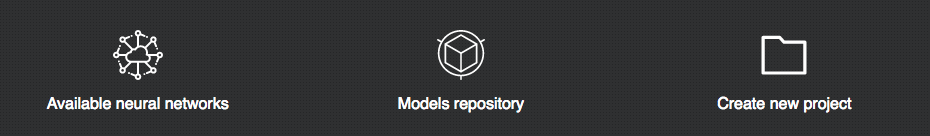
\includegraphics[scale=0.5]{components/5/img/n2sky_tools.png}
  \caption{N2Sky Main Module. Available user tools}
  \label{fig:n2sky_tools}
\end{center}
\end{figure}

In figure \ref{fig:n2sky_tools} the available tools component is displayed in a horizontal layout. Every item has an SVG icon and caption under it. The tools contain following functionalities: 
\begin{itemize}
\item \emph{Available neural network.} Reference to the available repositories view.  
\item \emph{Model repository.} Reference to the model repository view.
\item \emph{Create a new project.} On click of this time the popup window will be initialized as it displayed in figure \ref{fig:popupcreatenewproject}.


\begin{figure}[H]
\begin{center}
  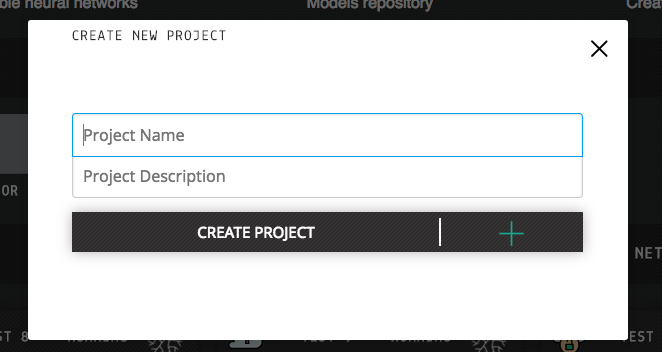
\includegraphics[scale=0.5]{components/5/img/popupcreatenewproject.png}
  \caption{N2Sky Main Module. Create New Project Popup}
  \label{fig:popupcreatenewproject}
\end{center}
\end{figure}


The following popup modal window contains components:
\begin{itemize}
\item \emph{Project Name} field, which represents a short title of the project.
\item \emph{Project Description} field with a short description of the project, which will be used for the semantic search.  
\item \emph{Create Project} button, which created a project with filled up form.
\end{itemize}

After creating the project it will automatically appear in the dashboard. 

\end{itemize}

\subsubsection{User Projects}

User projects is a grid with projects. Every project is represented as a folder with a caption under it as it displayed in figure \ref{fig:n2sky_dashboard_projects}. On click, the user will be redirected to the particular project. 

\begin{figure}[H]
\begin{center}
  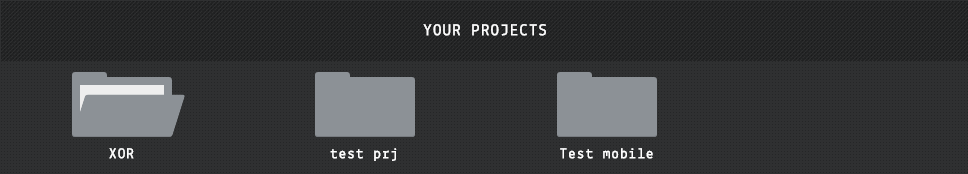
\includegraphics[scale=0.5]{components/5/img/n2sky_dashboard_projects.png}
  \caption{N2Sky Main Module. User projects grid}
  \label{fig:n2sky_dashboard_projects}
\end{center}
\end{figure}

 \subsubsection{The User Neural Networks and Models Overview}
 
 The component is displaying the neural networks of the user, which either created from paradigm or own contributed neural networks. The component contains following subcomponents:
 \begin{itemize}
\item \emph{Neural networks filtering bar.}
The filtering bar is a navigation as well as neural networks filtering subcomponent as is shown in figure \ref{fig:n2sky_filtering_bar}. The subcomponent allows the user to filter through neural networks depending on permissions. 

\begin{figure}[htbp]
\begin{center}
  
\includegraphics[scale=0.5]{components/5/img/n2sky_filtering_bar.png}
  \caption{N2Sky Main Module. Neural networks filtering bar.}
  \label{fig:n2sky_filtering_bar}
\end{center}
\end{figure}

The following filters are available: 
\begin{itemize}
\item \emph{Your networks.} The filter shows the running and not running neural networks of the logged in user. 
\item \emph{Your running networks.} The representation only of the user's running neural networks.
\item \emph{Saved networks.} Only saved neural networks of the users. The list will show the saved neural networks across all projects of the user.
\item \emph{All Networks}. List of all networks on the N2Sky. This filter is available only for the system administrator.
\end{itemize}
\item{The neural networks grid.} The grid, which contains custom UI components that the particular neural network. Every grid item contains the following information:
\begin{itemize}
\item The title of the neural network
\item The status tither running or not running. If the instance is running the N2Sky icon will spin, if not it will be grey without movements. 
\item The short description of the neural network
\item Application field
\item Network type
\item Problem type
\item Created by user
\item Details and actions button, which redirect the user to the page with detailed information of the neural network. 
\end{itemize}

\item{Navigation bar.} The bar under neural networks which contains the navigation buttons and "Chained/Unchained" mode.
\begin{itemize}
\item \emph{Unchained mode} is a mode where all trained model of displayed neural networks will be shown.
\item \emph{Chained mode} is a mode where only the trained models of the chosen neural network will be shown. In the chained mode, the user has to click on the particular neural network to see the trained models. 
\end{itemize}

\item{Trained models table.} The table with trained models, which contained also filtering and searching bar.
The filtering and searching bar allows to perform a semantic search across trained models and contains following filters:
\begin{itemize}
\item Trained by field available only for contributor user and system administrator.
\item Only Copy checkbox
\item Only Trained checkbox means to show only the trained models where the training is finished.
\item Show others modes checkbox will display the trained models from other users. The checkbox available only to the system administrator.
\end{itemize}

The table itself contains short information about the trained models. On click, the user will be redirected to the detailed overview of the trained model.

\end{itemize}

\subsection{The User Project Dashboard}\label{The user projects dashboard}
The user project dashboard is the dashboard, which suitable for any types of users. It is possible to create and manage own neural networks directly from the dashboard as it is shown in figure \ref{fig:projects_dsahboard}.

\begin{figure}[H]
\begin{center}
  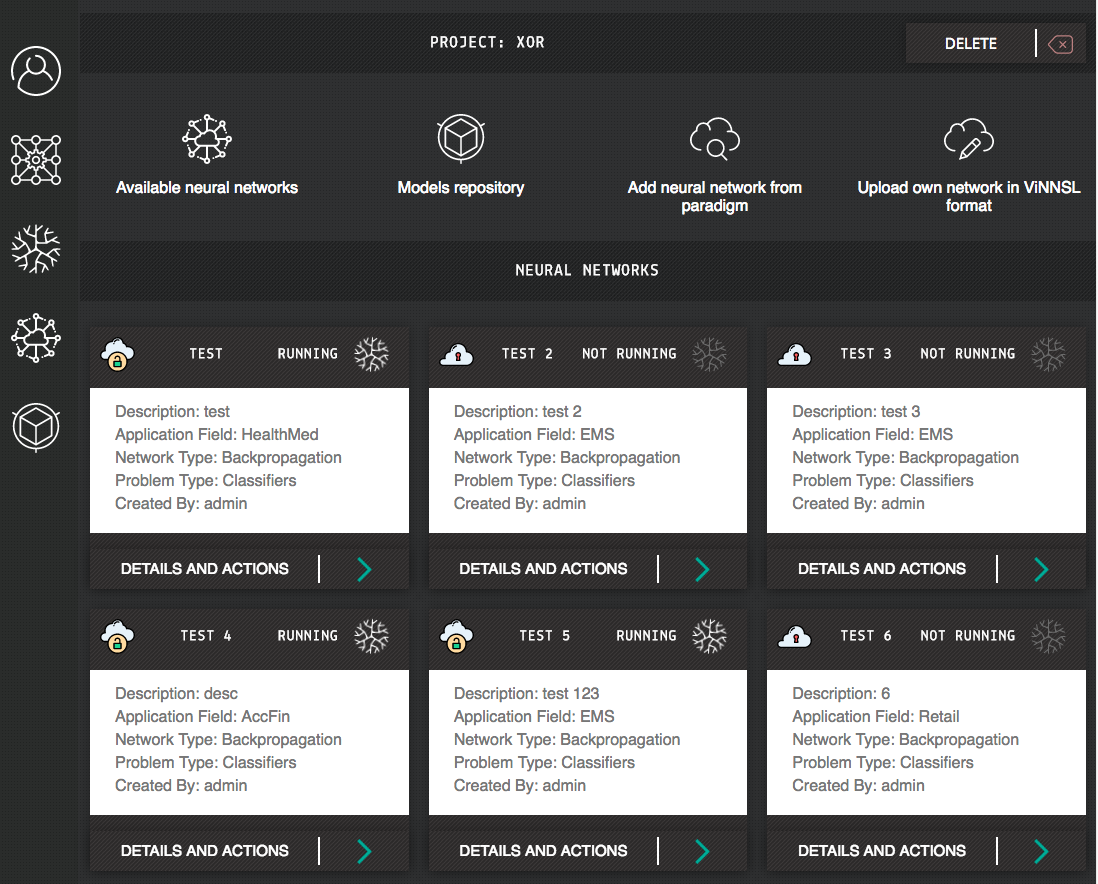
\includegraphics[width=\linewidth]{components/5/img/projects_dsahboard.png}
  \caption{N2Sky User Project Dashboard}
  \label{fig:projects_dsahboard}
\end{center}
\end{figure}

As any other dashboards in N2Sky, the project dashboard contains the available tools and the grid of items.
On the top of the dashboard, the title and the delete button is located. It is possible to delete project only for project owner or system administrator. 

\subsubsection{Available Tools} 

The available tools is a common functionality, which is necessary for project dashboard. Every tool contains an SVG icon and caption underneath as it displayed in figure \ref{fig:projecttools}. 

\begin{figure}[htbp]
\begin{center}
  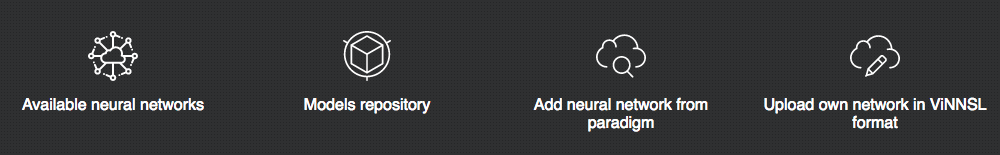
\includegraphics[width=\linewidth]{components/5/img/project_tools.png}
  \caption{N2Sky Project Dashboard. Available tools}
  \label{fig:projecttools}
\end{center}
\end{figure}

The following tools are available for all types of users:
\begin{itemize}
\item \emph{Available neural network.} Reference to the available repositories view.  
\item \emph{Model repository.} Reference to the model repository view.
\item \emph{Add neural network from the paradigm.} Will redirect to the creation of neural network from existing paradigm page. 
\item \emph{Upload own network in ViNNSL format} is mostly used by contributor user since the user needs to know the ViNNSL language. On click, the popup will be initialized as it is shown in figure \ref{fig:upload_vinnsl_popup}. 

\begin{figure}[htbp]
\begin{center}
  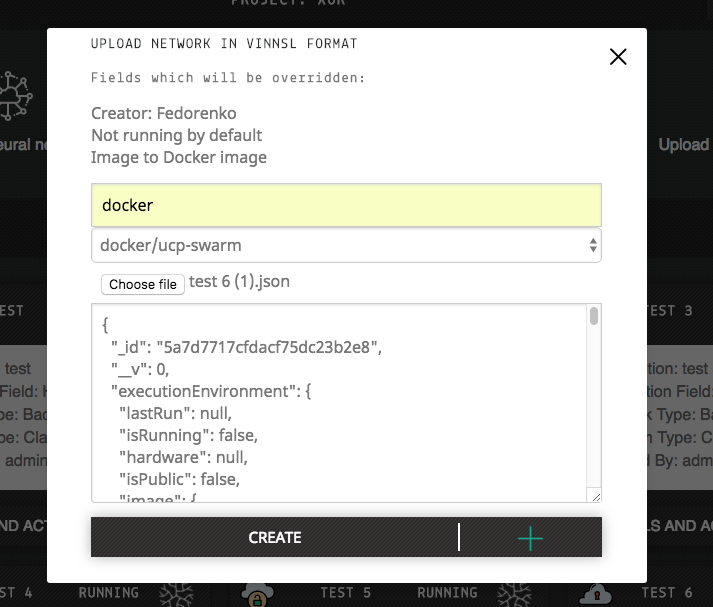
\includegraphics[scale=0.5]{components/5/img/upload_vinnsl_popup.png}
  \caption{N2Sky Project Dashboard.Upload own network in ViNNSL format}
  \label{fig:upload_vinnsl_popup}
\end{center}
\end{figure}

The popup contains following components:
\begin{itemize}
\item The information block about the following operation. The block shows, which fields are going to be overridden namely: the creator field, image information and it will be not running by default. 
\item The Docker username field, which references on the username in Docker Hub repository. After the name will be entered the available images list will be listed. 
\item The Docker image combo box is a list of available images of chosen Docker Hub user.  This image will be used for creating neural network paradigm.
\item The Upload field. The user needs to choose from local machine the neural network paradigm, which is described in ViNNSL XML or JSON format.
\item The text field will show the preview of uploaded neural network paradigm in ViNNSL format.
\item Create button will process the form and create the neural network paradigm. After creation, the user will be redirected to the neural network details page. 
\end{itemize}

\subsubsection{Neural Networks Grid}

The neural networks grid represents a list all neural network which was created or copied from other users. Every grid item contains brief information about the neural network:
\begin{itemize}
\item The title of the neural network
\item The status tither running or not running. If the instance is running the N2Sky icon will spin, if not it will be grey without movements. 
\item The short description of the neural network
\item Application field
\item Network type
\item Problem type
\item Created by user
\item Details and actions button, which redirect the user to the page with detailed information of the neural network. 
\end{itemize}

\subsubsection{Saved Trained Models}

The table with saved trained models is located at the bottom of project dashboard as it is shown in figure \ref{fig:saved_trained_models_project}.

\begin{figure}[H]
\begin{center}
  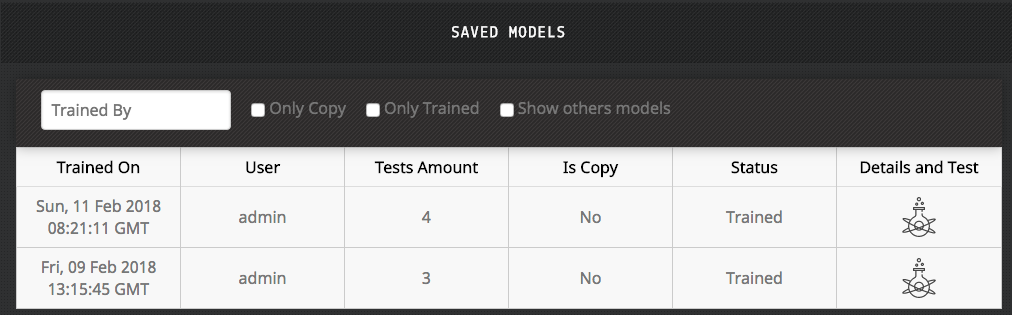
\includegraphics[width=\linewidth]{components/5/img/saved_trained_models_project.png}
  \caption{N2Sky Project Dashboard. Saved trained models}
  \label{fig:saved_trained_models_project}
\end{center}
\end{figure}

This table represents the copied trained models into the particular project. It is possible to perform the semantic search against trained models, the same approach is used in N2Sky Main Dashboard. 

\end{itemize}


\subsection{Three Steps View}\label{Three steps view}

Robert Browning in his poem "Andrea del Sarto" said: "Less is mode", which became an inspiration of the "Three steps view". It was derived from the simplicity of the arbitrary user. The idea behind to make possible to create the neural network from the paradigm within only three steps. After creation of the neural network reuse the same three steps to provide the overview of the created neural network.

The following steps have to be achieved in order to create the neural network from the paradigm:  the neural network description, the neural network structure, and the neural network training.

\subsubsection{The Neural Network Description}

When the user just entering to three step view, the fist what he will see it is "The Network Description" tab. In this tab, the user has to choose propagation method which is available on N2Sky. After choosing some propagation method the metadata from the ViNNSL template will be loaded. The metadata is represented as a form as is shown in figure \ref{fig:nn_desc_3_steps}

\begin{figure}[H]
\begin{center}
  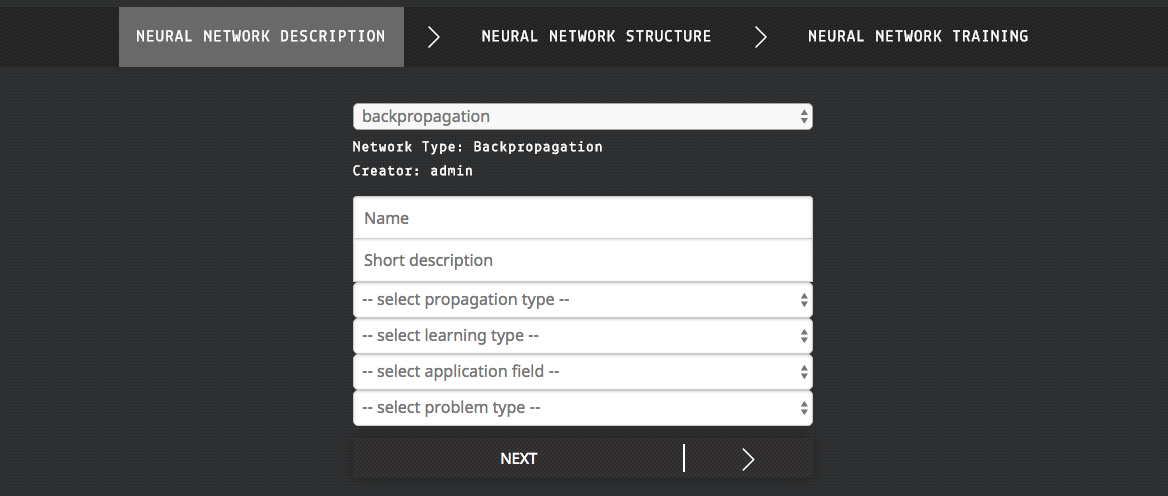
\includegraphics[width=\linewidth]{components/5/img/nn_desc_3_steps.png}
  \caption{Three Steps View. The Neural Network Description}
  \label{fig:nn_desc_3_steps}
\end{center}
\end{figure}

The mandatory metadata from the ViNNSL template is:
\begin{itemize}
\item Name of the neural network
\item Shot description
\item Propagation type
\item Learning type
\item Application field
\item Problem type
\end{itemize}

This data can be customized on demand. Any additional field in metadata of ViNNSL template will be reflected in this form.


After filling up the form, the user will be redirected to the "Neural Network Structure" tab.

\subsubsection{The Neural Network Structure}

The neural network structure field represents the structure of the neural network, which can be customized. It is also possible to set the connections between the layers and nodes. 

When the user entering to this tab he will so only three types of layers: 
\begin{itemize}
\item \emph{Input Layer}, which represents the amount of the nodes in the input layer.
\item \emph{Hidden Layers} can be multidimensional. It has the matrix structure, it means it is possible to choose multiple layers and multiple nodes. The amount of nodes does not have to be equal in each layer.
\item \emph{Output Layer} is a layer, which represents the number of nodes for output. This layer has to validate, because of the difference between neural networks. 
\end{itemize}

After choosing the correct numbers of the layers and nodes the visual representation will be shown as it displayed in figure \ref{fig:nn_structure_3_steps}.


\begin{figure}[htbp]
\begin{center}
  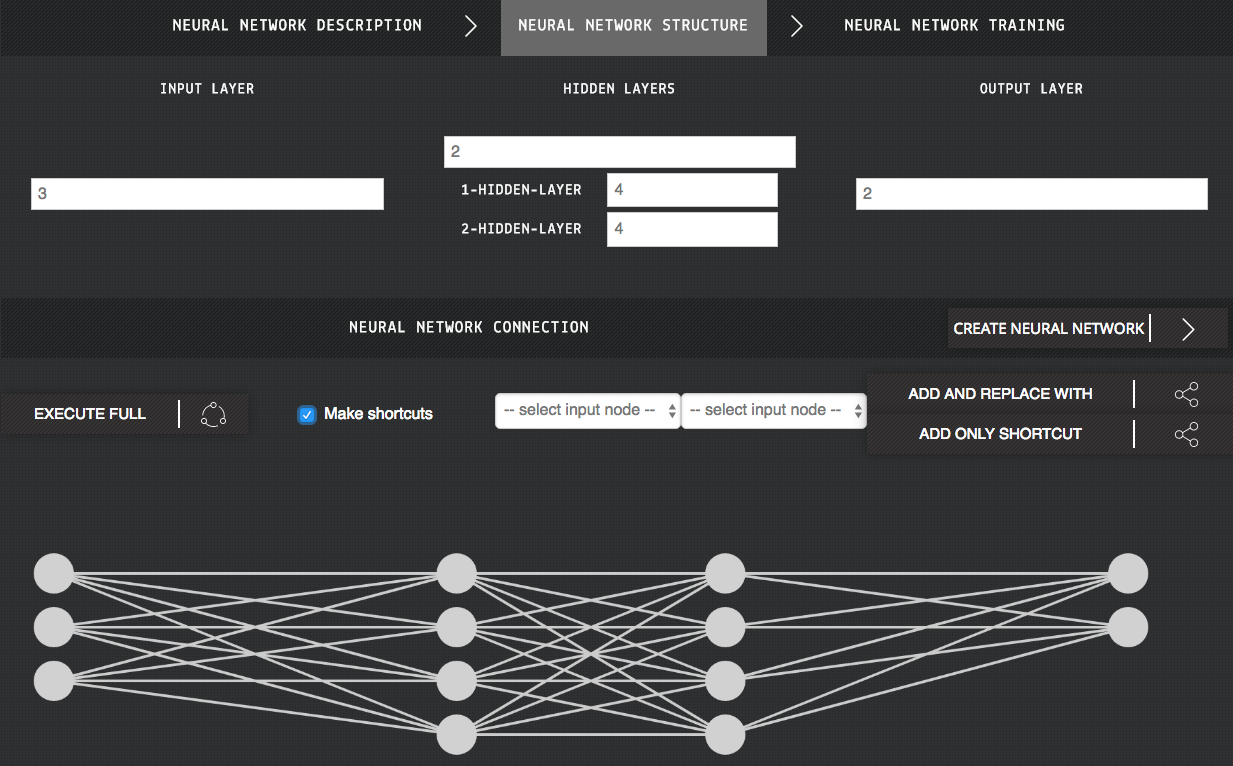
\includegraphics[width=\linewidth]{components/5/img/nn_structure_3_steps.png}
  \caption{Three Steps View. The Neural Network Structure with full connection}
  \label{fig:nn_structure_3_steps}
\end{center}
\end{figure}

The next step is to connect the nodes. Following connections are possible:

\begin{itemize}
\item \emph{Full Connection}. The nodes are full connected when they have the connection to all activation with other layers. This is standard approach in every neural network. The matrix multiplication followed be the bias offset. \cite{nn_connection}. This connection is possible to execute by clicking on "Execute full connection" button as is shown in figure \ref{fig:nn_structure_3_steps}.
\item \emph{Pure Shortcut.} Shortcut connection is also called skip connection. With this connection enables unimpeded information flow. This connection if adding the direct connection to other layers. This approach can gain results by training. \cite{shortcuts_nn} With pure connection it is possible to make some direct connection, it will also remove the full connection to the chosen node.
\item \emph{Only shortcut.} It is the same approach as by pure shortcut, except the full connection still enabled. 
\end{itemize}

In order to make shortcuts connection more understandable, they are will be immediately visualized as is shown in figure \ref{fig:connection_3_steps}. In this example, the first input node has pure shortcut connection with a second hidden layer and the third input node has only shortcut connection with output layer, the gull connection with this node remains the same.

\begin{figure}[htbp]
\begin{center}
  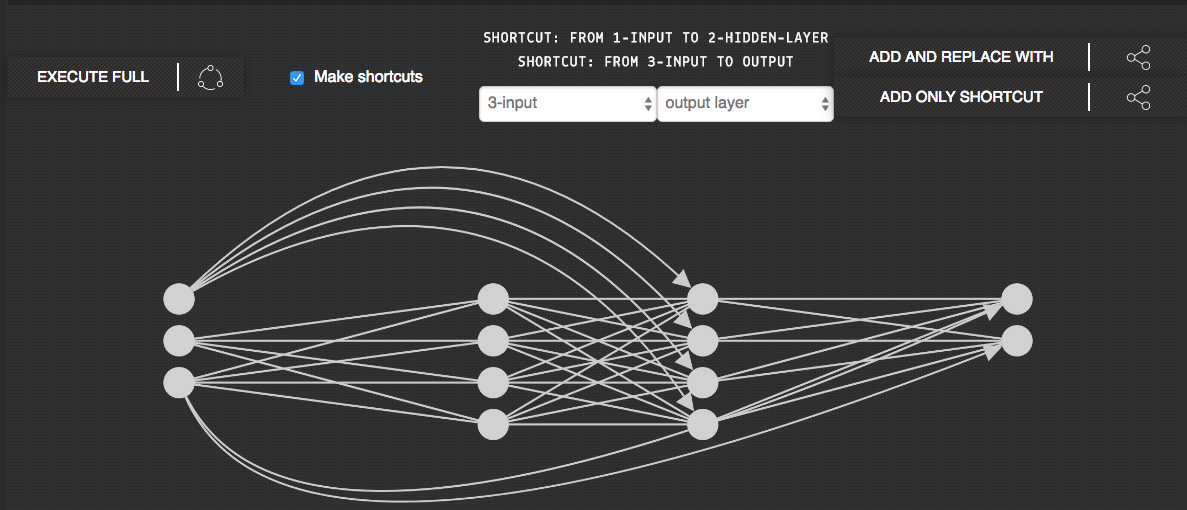
\includegraphics[width=\linewidth]{components/5/img/connection_3_steps.png}
  \caption{Three Steps View. The shortcut connections}
  \label{fig:connection_3_steps}
\end{center}
\end{figure}

After creating the neural network the user will be redirected to the "Neural Network Training" tab. The all other tabs are clickable, but is it not possible to change either metadata or the structure of the neural network.

\subsubsection{The Neural Network Training}

One of the most important steps in three-step view workflow, because from this tab is possible to perform some testing against the newly created neural network. The tab is multifunctional and scalable on permissions of the particular user as is shown in figure \ref{fig:training_3_steps}.

\begin{figure}[H]
\begin{center}
  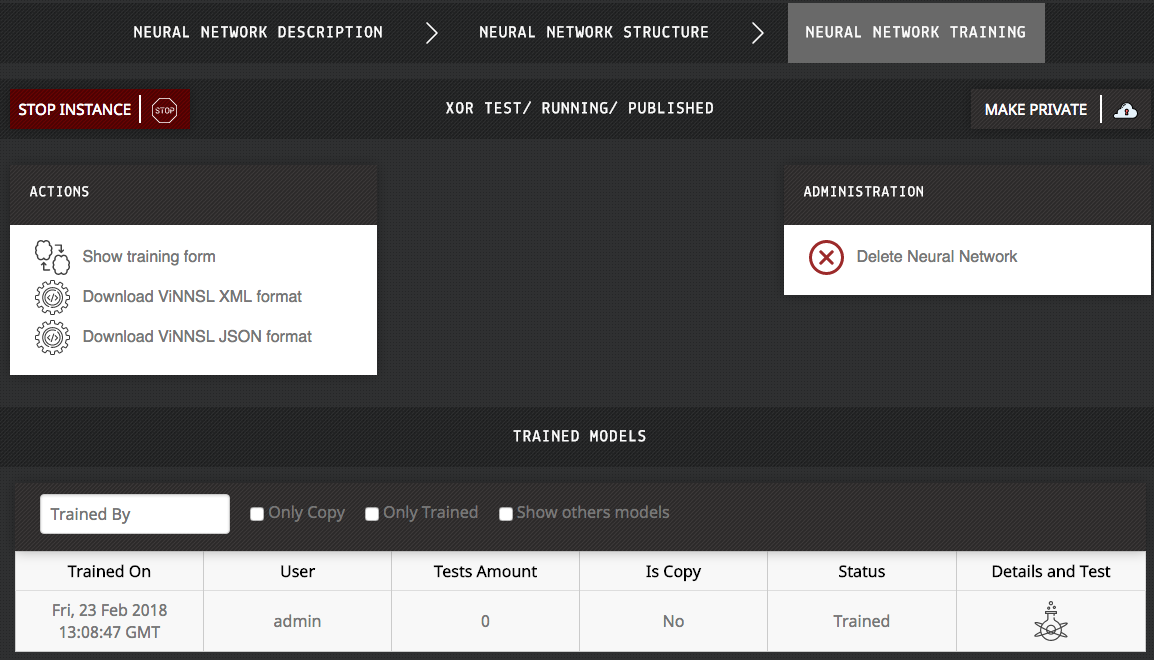
\includegraphics[width=\linewidth]{components/5/img/training_3_steps.png}
  \caption{Three Steps View. The Neural Network Training.}
  \label{fig:training_3_steps}
\end{center}
\end{figure}

There are few components which are available to the user:
\begin{itemize}
\item \emph{Administration.} This block is available only to neural network owner and the system administrator. The following operations are possible to perform from this block:
\begin{itemize}
\item \emph{Run the instance.} Without running the instance it is not possible to perform any testing. The user can run the neural network instance on N2Sky Cloud or if it his own neural network he can deploy on his own publicly available cloud as is shown in figure \ref{fig:run_instance_3_steps}. 

\begin{figure}[H]
\begin{center}
  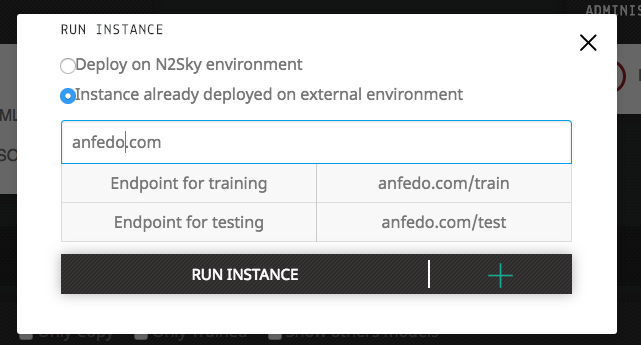
\includegraphics[scale=0.5]{components/5/img/run_instance_3_steps.png}
  \caption{Three Steps View. The Neural Network Training. Run instance}
  \label{fig:run_instance_3_steps}
\end{center}
\end{figure}

Only two endpoints are available:
\begin{itemize}
\item \emph{/train} - for training the neural network. This endpoint has to accept ViNNSL-formatted neural network description and the training data. 
\item \emph{/test} - for evaluating the trained model. Has to accept only testing data.
\end{itemize}
Detailed information of API can be found in Development chapter \autoref{API Documentation}.
\item \emph{Stop the instance.} If the instance is running it is possible to stop it. The instance will be removed from the N2Sky cloud if it was deployed there.
\item \emph{Publish the neural network.} The user can publish running neural network. In this case, the neural network will be available in neural network repository and its trained models also. The other users can copy published neural networks in their own projects. 
\item \emph{Delete the neural network.} If the neural network owner or administrator will decide to remove the neural network, then the all trained models and testing data also will be removed. The neural network will not be published anymore and the running instance will be removed.
\end{itemize}
\item \emph{Actions.} The actions are available for every user if the neural network is published. The following actions can be performed:
\begin{itemize}
\item \emph{Show training form.} On click the training form will be expanded as is shown in figure \ref{fig:expand_training_form}

\begin{figure}[H]
\begin{center}
  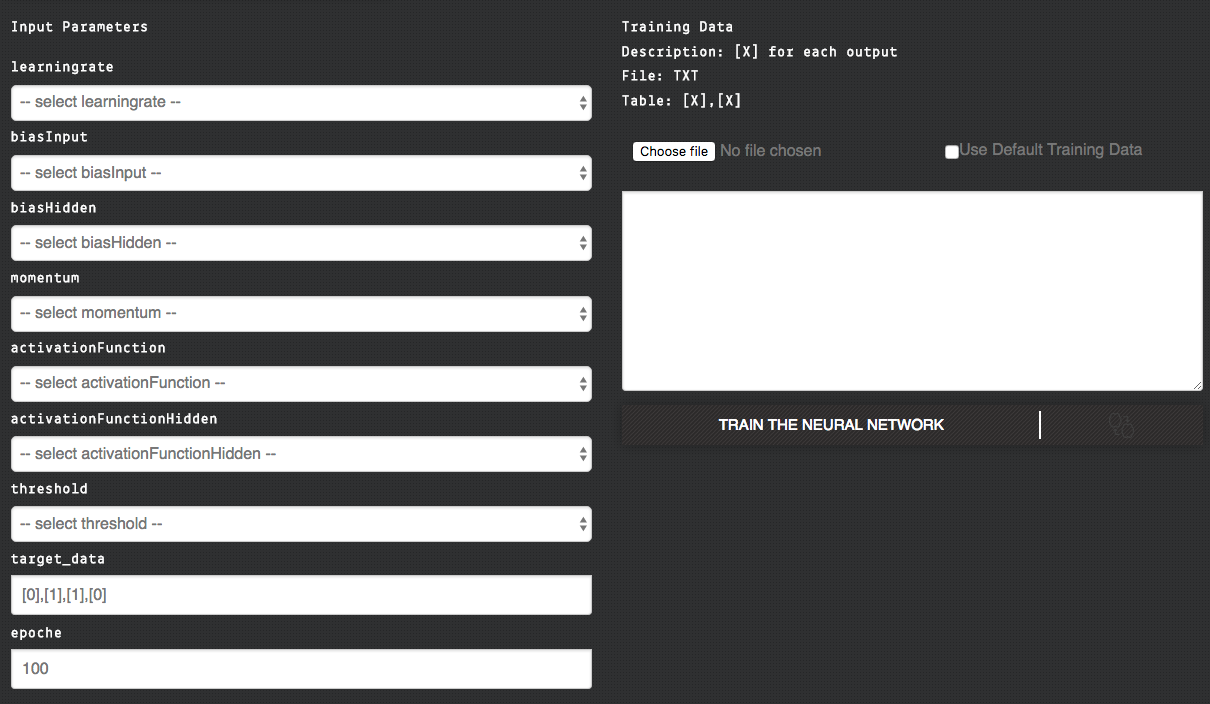
\includegraphics[width=\linewidth]{components/5/img/expand_training_form.png}
  \caption{Three Steps View. The Neural Network Training. Training form}
  \label{fig:expand_training_form}
\end{center}
\end{figure}

The form data is fetched by reflection from ViNNSL Template, namely from input parameters. If there are possible values set in particular the combo box will be shown, if there is only one default value set, the free text field will be displayed.  On the right side, there is training data information box. It is possible to upload own training data or chose default training data.

\item \emph{Download ViNNSL XML format}
\item \emph{Download ViNNSL JSON format}
\end{itemize}

\item \emph{Trained Models Table} is similar to the table in the table in the "Model Repository." It is possible to perform the semantic search against existing trained models. The user can see the status of the training and on the clock of the particular model, he will be redirected to the testing view and detailed information about training.

\end{itemize}

\subsubsection{Training Results and the Model Evaluation}\label{Training results and the model evaluation}

The testing is a part of the model evaluation that is why it is under three-step-view workflow. The training results and the model evaluation page is an underline of the workflow. From this page, the user can observe chosen training model, study the training graph and evaluate trained model as is shown in figure \ref{fig:testing_model}.

\begin{figure}[htbp]
\begin{center}
  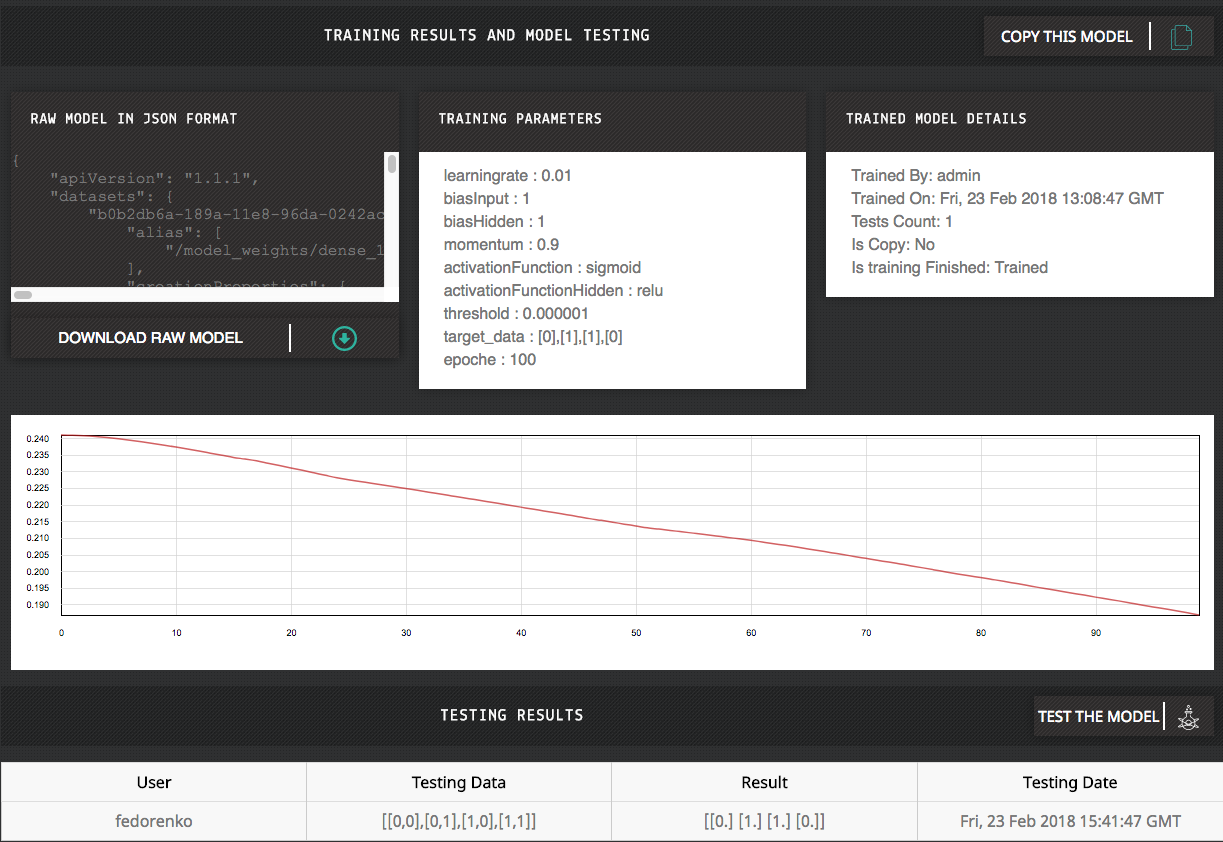
\includegraphics[width=\linewidth]{components/5/img/testing_model.png}
  \caption{Three Steps View. Training Results and the Model Evaluation}
  \label{fig:testing_model}
\end{center}
\end{figure}

The page view contains following elements:
\begin{itemize}
\item \emph{Functional bar} consists of the title itself and the functional copy of the project button. The functionality is pretty the same as copying the neural network to the own project from the neural network repository. The user has to choose the project in popup modal window and then perform copying as is shown in figure \ref{fig:copy_model}. It is possible to copy the trained model into multiple projects. 

\begin{figure}[htbp]
\begin{center}
  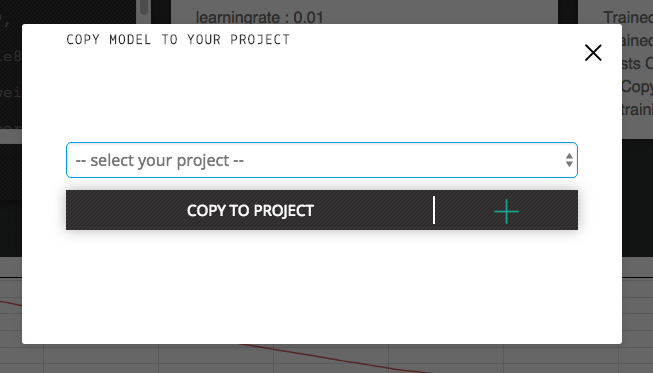
\includegraphics[scale=0.5]{components/5/img/copy_model.png}
  \caption{Three Steps View. Training Results and the Model Evaluation. Copy model into own project.}
  \label{fig:copy_model}
\end{center}
\end{figure}

\item \emph{Row model in JSON format}, which gives an overview of the trained model. The model can be viewed directly from UI as well as it is possible to download it and review from Desktop or mobile device. 
\item \emph{Training parameters} is the input parameters, with which the neural network was trained. The parameters can differentiate from paradigm to paradigm.
\item \emph{Trained model detail} is the metadata of the trained model. Namely, timestamp event metadata information. It contains following data:
\begin{itemize}
\item Trained by user information
\item Trained on timestamp
\item Tests count (the tests, which are already performed)
\item Is a copy information
\item Is training finished information
\end{itemize}

\item \emph{Graph}, which represents epochs in x-axis and error on the y-axis. If the neural network still in process of the training the graph will move with it. 
\item \emph{Test the model} button will initiate the testing popup modal window as is shown in figure \ref{fig:model_testing}. The user has to choose the testing data, it is possible to use the default values.

\begin{figure}[htbp]
\begin{center}
  \includegraphics[scale=0.5]{components/5/img/model_testing.png}
  \caption{Three Steps View. Training Results and the Model Evaluation. The model testing.}
  \label{fig:model_testing}
\end{center}
\end{figure}

\item \emph{Testing results} it a table with testing results. The user can see only his own testing results if the user is the neural network owner or the system administrator he can see the results from other users also. The table has following columns:
\begin{itemize}
\item The user who performs the testing 
\item The testing data
\item Results (output)
\item Testing Date
\end{itemize}


\end{itemize}





\subsection{Neural Networks Repository}\label{Neural Networks Repository}

The neural repository is representing a repository, where any user can find and reuse available neural network. The neural network repository contains the search bar and the grid with the published neural networks as it displayed in figure \ref{fig:nn_repository}. If the neural network is published by the neural network owner, it is automatically added to the repository. It is important to mention, that only published networks of other users will be displayed. 

\begin{figure}[H]
\begin{center}
  \includegraphics[width=\linewidth]{components/5/img/nn_repository.png}
  \caption{N2Sky Neural network repository}
  \label{fig:nn_repository}
\end{center}
\end{figure}


\begin{enumerate}
\item \emph{Searching bar.} With the searching bar is possible to perform the semantic search against available neural networks in the repository. It is possible to search by: 
\begin{itemize}
\item Name of the neural network
\item Description of the neural network
\item Network Type
\item Problem Type
\end{itemize}

Each field is case insensitive. The inquiry will be processed in converted in order to give most reliable results. 

\item \emph{Networks grid} is a grid, which represents the published neural networks. It has 3 columns in Desktop version and 1 in the mobile version. Every grid item has a title, which contains following components:
\begin{itemize}
\item The save button-icon. The button is displayed as a start. If the star has a color then the neural network already saved. If the icon is transparent it means that it is possible to save the neural network. On click of the transparent button, the popup modal window will appear as is shown in figure \ref{fig:copy_nn}. From the modal window, the user can choose available projects, where he can copy chosen neural network. 


\begin{figure}[htbp]
\begin{center}
  \includegraphics[scale=0.5]{components/5/img/copy_nn.png}
  \caption{N2Sky Neural network repository. Copy the neural network.}
  \label{fig:copy_nn}
\end{center}
\end{figure}

\item Availability of the neural network. Can be public (green), private (red) and restricted (yellow). The arbitrary user can observer only public neural networks, the administrator can observe any neural network in N2Sky.  

\item The name of the neural network
\item The running status. Can be running and not running.
\item The running icon. Can be spinning icon for running and standing alone is for not running the network.
\end{itemize}

Besides details and actions button, which redirect the user to neural network details, the brief network information is deployed:
\begin{itemize}
\item Short description
\item Application field
\item Network type
\item Problem type
\item Created by
\end{itemize}

\end{enumerate}

\subsection{Models Repository}\label{Models Repository}

The modal repository is similar to neural networks repository but contains only trained models. The structure is also different. Because of the big amount of the trained models the models are displayed in the table as is shown in figure \ref{fig:model_repo}. 

\begin{figure}[H]
\begin{center}
  \includegraphics[width=\linewidth]{components/5/img/model_repo.png}
  \caption{N2Sky Models Repository}
  \label{fig:model_repo}
\end{center}
\end{figure}

The model repository page view contains models table and a brief description of  the chosen model:
\begin{itemize}
\item \emph{Trained model table} is consist of the search bar and table itself.
\begin{itemize}
\item The search bar gives possibility perform the semantic search against available trained models. It has following filters:
\begin{itemize}
\item Trained by
\item Only copy checkbox
\item Show other models checkbox
\end{itemize}
\item The table. On clock of the table, the short description of the trained model will be opened. The table contains following elements:
\begin{itemize}
\item Trained on (timestamp)
\item User
\item Tests amount
\item Is copy
\item Status
\item Details and tests
\end{itemize}
\end{itemize}

\item \emph{The short description} is located on the right side of the page. When the user just entering to the page there will be only notification, which motivates the user to chose the model. After choosing it, the view will be replaced with a short description as is shown in figure \ref{fig:short_desc}.

\begin{figure}[H]
\begin{center}
  \includegraphics[width=\linewidth]{components/5/img/short_desc.png}
  \caption{N2Sky Models Repository. Short Description}
  \label{fig:short_desc}
\end{center}
\end{figure} 

The description contains following components:
\begin{itemize}
\item Title, which consists of the ID of the model and button, which will redirect to details of the chosen model.
\item The list of the input parameters. This list can differ, depending on neural network paradigm. 
\item The raw model, which can be downloaded. 
\end{itemize}

\end{itemize}

\section{Tutorial}\label{Tutorial}

The tutorial describes few main cases of the arbitrary user, neural network engineer and contributor user. The use cases will be described in UML  Activity Diagram. The details will be skipped, only the main function will be described.  

\subsection{Using Network and Model Repositories}\label{Using Network and Model Repositories}

\begin{figure}[htbp]
\begin{center}
  \includegraphics[width=\linewidth]{components/tutorial/img/training_arbitrary.jpg}
  \caption{Tutorial. Activity Diagram of using Network and Model Repositories}
  \label{fig:training_arbitrary}
\end{center}
\end{figure} 

\subsection{Creation of the neural network from the existing paradigm}\label{Creation of the neural network from the existing paradigm}

This case is related to neural network engineer user. 

\begin{figure}[htbp]
\begin{center}
  \includegraphics[width=\linewidth]{components/tutorial/img/tutorial_engeneer.jpg}
  \caption{Tutorial. Activity Diagram of creation the neural network from the existing paradigm}
  \label{fig:tutorial_engeneer}
\end{center}
\end{figure} 

\subsection{Upload own neural network paradigm}\label{Upload own neural network paradigm}


\begin{figure}[htbp]
\begin{center}
  \includegraphics[width=\linewidth]{components/tutorial/img/tutorial_contribut.jpg}
  \caption{Tutorial. Activity Diagram of upload own neural network paradigm}
  \label{fig:tutorial_contribut}
\end{center}
\end{figure} 
\section{User Cases}\label{User Cases}

\section{Developer Guide}\label{Developer Guide}

\subsection{System Configuration}\label{System configuration}

\subsubsection{Prerequirements}\label{Prerequirements}

Following technologies has been used:

\begin{table}[H]
\centering
\caption{My caption}
\label{my-label}
\begin{tabular}{|l|l|}
\hline
\textbf{Technology} & \textbf{Version} \\ \hline
Docker CE           & 17.12.1-ce       \\ \hline
MongoDB             & 3.6              \\ \hline
NodeJS              & 7.0.0            \\ \hline
npm                 & 4.2.0            \\ \hline
Prometheus          & 2.0.0            \\ \hline
node\_exporter      & 0.16.0-rc.0      \\ \hline
Alertmanager        & 0.15.0-rc.0      \\ \hline
React               & 15.6.1           \\ \hline
Redux               & 3.7.2            \\ \hline
\end{tabular}
\end{table}

Every N2Sky service has "package.json" file on the root of the project. This file contains versions of all used packages in particular service.
\subsubsection{Setting Up the Database}\label{database setup}

N2Sky uses non-relational database MongoDB, which is running in Docker container. 

First of all the developer has to create  the mongo database container:

 \begin{lstlisting}
	docker run -d -p 27017:27017 --name database \
	 -v ~/dataMongo:/data/db mongo
\end{lstlisting}

It will start the mongo database Docker container on port 27017. 
It is possible to remap ports with the flag "-p".

The second step is to configure N2Sky database:

\emph{Login into container:}  
 \begin{lstlisting}
docker exec -it database mongo
\end{lstlisting}

\emph{Create database superuser:}
 \begin{lstlisting}
 
db.createUser(
	{ user: 'admin', pwd: 'password',
	 roles: [
	 	{ role: "userAdminAnyDatabase", db: "admin" }
			 ] });

\end{lstlisting}



\emph{Create database:}
 \begin{lstlisting}
use n2sky;
\end{lstlisting}


\emph{Create database n2sky user:}
 \begin{lstlisting}
 
db.createUser({user:"n2sky", pwd:"password", roles:['dbOwner']})

\end{lstlisting}

\emph{Create system administrator:}
 \begin{lstlisting}
 
db.users.insert({
   "name":"admin",
   "password":"password",
   "email":"admin@test.com",
   "type":"admin",
   "active":true
});

\end{lstlisting}


\emph{For production version it is recommended to enable authentication:}
 \begin{lstlisting}
 
 	docker rm -f database
 
	docker run -d -p 27017:27017 --name database \
	 -v ~/dataMongo:/data/db mongo mongod --auth

\end{lstlisting}



\subsubsection{Setting Up the Cloud Web Service}\label{cloud setup}

\emph{Clone the project from the repository}
 \begin{lstlisting}
git clone https://github.com/latyaodessa/n2sky-services.git 
\end{lstlisting}

\emph{Go to service Dockerfile}
 \begin{lstlisting}
cd n2sky-services/services
\end{lstlisting}

\emph{Build the Docker image}

Dockerfile:
 \begin{lstlisting}
FROM node:7
WORKDIR /app
COPY package.json .
RUN npm install
RUN npm install -g forever
COPY . /app
CMD forever -c 'node --harmony'  server.js
EXPOSE 8080
\end{lstlisting}

Command: 
 \begin{lstlisting}
docker build -t cloud:1 .
\end{lstlisting}


\emph{Run the service Docker container}
 \begin{lstlisting}
docker run -d -p 9595:8080 --name cloud cloud:1
\end{lstlisting}


Important to check the host and the port of the database. 
If something goes wrong and the port or the host is changed in n2sky project developer can edit it.
The rest API endpoint host located in \emph{service/config/database.js}

\subsubsection{Setting Up the Model Repository Service}\label{model setup}

\emph{Clone the project from the repository}
 \begin{lstlisting}
git clone https://github.com/CN2Sky/modelRepository.git
\end{lstlisting}

\emph{Go to service Dockerfile}
 \begin{lstlisting}
cd modelRepository
\end{lstlisting}

\emph{Build the Docker image}

Dockerfile:
 \begin{lstlisting}
FROM node:7
WORKDIR /app
COPY package.json .
RUN npm install
RUN npm install -g forever
COPY . /app
CMD forever -c 'node --harmony'  server.js
EXPOSE 8080
\end{lstlisting}

Command: 

 \begin{lstlisting}
docker build -t model:1 .
\end{lstlisting}


\emph{Run the service Docker container}
 \begin{lstlisting}
docker run -d -p 9092:8080 --name model model:1
\end{lstlisting}



\subsubsection{Setting Up the User Management Service}\label{user setup}

\emph{Clone the project from the repository}
 \begin{lstlisting}
git clone https://github.com/CN2Sky/user-management.git
\end{lstlisting}

\emph{Go to service Dockerfile}
 \begin{lstlisting}
cd user-management
\end{lstlisting}

\emph{Build the Docker image}

Dockerfile:
 \begin{lstlisting}
FROM node:7
WORKDIR /app
COPY package.json .
RUN npm install
RUN npm install -g forever
COPY . /app
CMD forever -c 'node --harmony'  server.js
EXPOSE 8080
\end{lstlisting}

Command: 

 \begin{lstlisting}
docker build -t user:1 .
\end{lstlisting}


\emph{Run the service Docker container}
 \begin{lstlisting}
docker run -d -p 9091:8080 --name user user:1
\end{lstlisting}



\subsubsection{Setting Up the N2Sky Frontend}\label{frontend setup}

\emph{Clone the project from the repository}
 \begin{lstlisting}
git clone https://github.com/latyaodessa/n2sky-services.git 
\end{lstlisting}

\emph{Go to service Dockerfile}
 \begin{lstlisting}
cd n2sky-services/frontend
\end{lstlisting}

\emph{Build the Docker image}
Dockerfile:
 \begin{lstlisting}
FROM node:7
WORKDIR /app
COPY package.json .
RUN npm install
COPY . /app
CMD npm run dev
EXPOSE 9593
\end{lstlisting}

Command:
 \begin{lstlisting}
docker build -t frontend:1 .
\end{lstlisting}


\emph{Run the service Docker container}
 \begin{lstlisting}
docker run -d -p 9593:9593 --name frontend frontend:1
\end{lstlisting}





\subsubsection{Setting Up the Backpropogation Neural Network}\label{backprop setup}

This neural network made for demonstration purposes. 

\emph{Clone the project from the repository}
 \begin{lstlisting}
git clone https://github.com/CN2Sky/backprop.git
\end{lstlisting}

\emph{Go to service Dockerfile}
 \begin{lstlisting}
cd backprop
\end{lstlisting}

\emph{Build the Docker image}

Dockerfile:
 \begin{lstlisting}
FROM debian:8

MAINTAINER Kamil Kwiek <kamil.kwiek@continuum.io>

ENV LANG=C.UTF-8 LC_ALL=C.UTF-8

RUN apt-get update --fix-missing && apt-get install -y wget bzip2 ca-certificates \
    libglib2.0-0 libxext6 libsm6 libxrender1 \
    git mercurial subversion

RUN echo 'export PATH=/opt/conda/bin:$PATH' > /etc/profile.d/conda.sh && \
    wget --quiet https://repo.continuum.io/archive/Anaconda2-5.0.1-Linux-x86_64.sh -O \
     ~/anaconda.sh && \
    /bin/bash ~/anaconda.sh -b -p /opt/conda && \
    rm ~/anaconda.sh

RUN apt-get install -y curl grep sed dpkg && \
    TINI_VERSION=`curl https://github.com/krallin/tini/releases/latest | \
    grep -o "/v.*\"" | sed 's:^..\(.*\).$:\1:'` && \
    curl -L "https://github.com/krallin/tini/releases/download/v \
    ${TINI_VERSION}/tini_${TINI_VERSION}.deb" > tini.deb && \
    dpkg -i tini.deb && \
    rm tini.deb && \
    apt-get clean

ENV PATH /opt/conda/bin:$PATH

# Jupyter has issues with being run directly: https://github.com/ipython/ipython/issues/7062
COPY backprop /root/

# Expose Ports for TensorBoard (6006), Ipython (8888)
EXPOSE 6006 8888 5000

WORKDIR "/root"

RUN pip install keras
RUN pip install tensorflow
RUN pip install h5json

CMD ["python", "server.py"]
\end{lstlisting}

Command: 

 \begin{lstlisting}
docker build -t backprop:1 .
\end{lstlisting}


\emph{Run the service Docker container}
 \begin{lstlisting}
docker run -d -p 6006:6006 -p 8888:8888 -p 5000:5000 --name backprop backprop:1
\end{lstlisting}







\subsubsection{Setting Up the Monitoring System}\label{Monitoring System setup}

To create custom image (OS: Ubuntu 16.04 Cloud version) with monitoring setup following steps has to be completed:

\emph{Clone the project from the repository}
 \begin{lstlisting}
git clone https://github.com/latyaodessa/n2sky-services.git 
\end{lstlisting}


\emph{Go to service Dockerfile}
 \begin{lstlisting}
cd n2sky-services/monitoring/prometheus
\end{lstlisting}

\emph{Build the Docker image}

Dockerfile:
 \begin{lstlisting}

FROM prom/prometheus:v2.0.0-beta.2
COPY alert.rules /etc/prometheus/alert.rules
COPY test.rules /etc/prometheus/test.rules
COPY node.rules /etc/prometheus/node.rules
COPY ./prometheus.yml /etc/prometheus/prometheus.yml

\end{lstlisting}

Command: 

 \begin{lstlisting}
docker build -t prometheus:1 .
\end{lstlisting}


\emph{Run the service Docker container}
 \begin{lstlisting}
docker run -d -p 9090:9090 prometheus:1
\end{lstlisting}


In case if developer want to see full stack he needs to deploy node\_exporter:

\emph{Clone the project from the repository}
 \begin{lstlisting}
git clone https://github.com/latyaodessa/n2sky-services.git 
\end{lstlisting}


\emph{Go to service Dockerfile}
 \begin{lstlisting}
cd n2sky-services/monitoring/node_exporter 
\end{lstlisting}

\emph{Run the service Docker container and start Monitoring}
 \begin{lstlisting}
docker build -t node_exporter . && \
docker run -d -p 9100:9100 node_exporter && \
cd ../prometheus && \
nohup ./prometheus > /dev/null 2>&1 &
\end{lstlisting}



 In the global configuration is possible to setup scare interval and evaluation interval.
global:
 
 \begin{lstlisting}
  scrape_interval:     15s 
  evaluation_interval: 15s 
\end{lstlisting}

Prometheus has to reference on Alert Manager, where messages will be published. 
 \begin{lstlisting}
alerting:
  alertmanagers:
  - static_configs:
    - targets:
       - localhost:9093
\end{lstlisting}

Every machine where Prometheus is installed can has its own alerting rules. In general alerting rules are located in the root folder of Prometheus.

 \begin{lstlisting}
rule_files:
   - "alert.rules"
   - "node.rules"
   - "test.rules"
\end{lstlisting}

Since there is a need to get more specific data, in N2Sky was decided to user Node Exporter Module. The reference on this module has to be added into configuration

 \begin{lstlisting}
- job_name: 'node'
    scrape_interval: 5s
    target_groups:
-	targets: ['localhost:9100']
\end{lstlisting}

Node Exporter Module has no configuration file. Prometheus listen the modules and scrap the data with a defined interval.

For deploying alert manager Docker containers technology is used.

\subsubsection{Setting Up Alert Management System}\label{Setting up Alert Management System}

All configuration of alert manager is written in YAML file. 
On the beginning SMTP, email sender should be configured. This would be used for sending notifications.

 \begin{lstlisting}
global:
  smtp_smarthost: 'localhost:25'
  smtp_from: 'alertmanager@example.org'
  smtp_auth_username: 'alertmanager'
  smtp_auth_password: 'password'
\end{lstlisting}

It is possible to define multiple Email templates and configure which template need to be loaded on which severe level. In configuration the path to templates need to be defined. 

 \begin{lstlisting}
templates: 
-	'/etc/alertmanager/template/*.tmpl'
\end{lstlisting}

When alerts are consumed they need to be converted using Email template and fired to the particular route. Every route has a receiver. 

 \begin{lstlisting}
route:
group_by: ['alertname', 'cluster', 'service']
group_wait: 30s
group_interval: 5m
repeat_interval: 3h 
receiver: team-X-mails
\end{lstlisting}

\begin{description}
\item[group\_by] Group by label. This way ensures that multiple alerts from difference cluster can be received
\item[group\_wait] Ensures that multiple alerts can be fired shortly after particular group is received.
\item[group\_interval] Interval between alert batches.
\item[Receiver] Unique name of receiver which is defined in configuration. 
\end{description}

Receiver it is a group of matching by regular expression events.

 \begin{lstlisting}
  routes:
- match_re:
      service: ^(foo1|foo2|baz)
    receiver: team-X-mails
\end{lstlisting}

Receiver can be defined by user configuration, it is an email where is alert notification will be send.

 \begin{lstlisting}
receivers:
- name: 'team-X-mails'
  email_configs:
  - to: 'team-X+alerts@example.org'
\end{lstlisting}

\paragraph{How to write alerting rules} 

The alerting rules are supporting simple query language, which looks very similar to Sequel Query Language.  
There are multiple possibilities how to work with alerting rules. The query language allows to use an expression and as a result to check an attribute of time series. 

 \begin{lstlisting}
ALERT HighLatency
 IF api_http_request_latencies_second{quantile="0.7"} > 1 
FOR 5m 
LABELS { severity="critical"} 
ANNOTATIONS {   summary = "High latency detected ",   description = "over limit? } 
\end{lstlisting}

Following notations should be considered be the creation of alerting rules:
\begin{itemize}
\item All queries starting with "ALERT" namespace. After it follows the name of alert, in this case, it is "HighLatency".  
\item "IF" is a condition "api\_http\_request\_latencies\_second", which based on Prometheus Tool expression.  Set of time series with this expression has one parameter it is "quantile". Reading condition as a whole can be translated into a human language like this: "Send an alert if latency request per second bigger then 0.7". 
\item "FOR" it is period of time how often this condition should be checked. 
\item "LABELS" shows a severity level. There are 3 types of severity:
\begin{itemize} 
        \item Critical
        \item Warning
        \item Page
     \end{itemize}
\item Every severity level can be defined on developer needs.
\item "ANNOTATIONS" shows a readable for human comments. There are two subsections: summary, which shows a short description of the event and description where detailed information about deviation can be written
\end{itemize}

For deploying alert manager Docker containers technology is used.

\emph{Clone the project from the repository}
 \begin{lstlisting}
git clone https://github.com/latyaodessa/n2sky-services.git 
\end{lstlisting}


\emph{Go to service Dockerfile}
 \begin{lstlisting}
cd n2sky-services/monitoring/alertmanager
\end{lstlisting}

\emph{Build the Docker image}

Dockerfile:
 \begin{lstlisting}

FROM prom/alertmanager:v0.10.0
COPY alertmanager.yml /etc/alertmanager/config.yml
ENTRYPOINT [ "/bin/alertmanager" ]
CMD        [ "-config.file=/etc/alertmanager/config.yml", \
             "-storage.path=/alertmanager" ]

\end{lstlisting}

Command: 

 \begin{lstlisting}
docker build -t alertmanager:1 .
\end{lstlisting}


\emph{Run the service Docker container}
 \begin{lstlisting}
docker run -d -p 9093:9093 alertmanager:1
\end{lstlisting}


\subsection{API Documentation}\label{API Documentation}

The API documentation will consist of three parts:
\begin{itemize}
\item Short description
\item The API endpoint
\item Example call
\item Response
\end{itemize}

\subsubsection{N2Sky Monitoring System API Documentation}\label{N2Sky Monitoring System API Documentation}

\begin{itemize}
\item \textbf{\textit{Get monitoring data with period from chosen server}}
\begin{itemize}
\item \emph{GET: /api/monitoring/:server/:query/:minus/:type/:step}
\\Parameters:
\begin{itemize}
\item :server - The server api or hostname, where monitoring is installed and running.
\item :query - query against monitoring data.
\item :minus - difference between current minus desired time.
\item :type - can be seconds, minutes, hours 
\item :step - the step between difference time and current time
\end{itemize}

\item \emph{Example call:}
 \begin{lstlisting}
http://192.168.0.102:9595/api/monitoring/192.168.0.105
/http_request_duration_microseconds/3/hours/15m
\end{lstlisting}

\item \emph{Response:}
 \begin{lstlisting}
{
        "metric": {
            "__name__": "http_request_duration_microseconds",
            "handler": "static",
            "instance": "localhost:9090",
            "job": "prometheus",
            "quantile": "0.5"
        },
        "values": [
            [
                1519558760,
                "NaN"
            ]
            ...
\end{lstlisting}
\end{itemize}

%%

\item \textbf{\textit{Get possible metrics}}
\begin{itemize}
\item \emph{GET: /api/monitoring/metrics/:host}
\\Parameters:
\begin{itemize}
\item :host - The server api or hostname, where monitoring is installed and running.
\end{itemize}

\item \emph{Example call:}
 \begin{lstlisting}
http://192.168.0.102:9595/api/monitoring/metrics/openstack
\end{lstlisting}

\item \emph{Response:}
 \begin{lstlisting}
[
    "ALERTS",
    "go_gc_duration_seconds",
    "go_gc_duration_seconds_count",
    "go_gc_duration_seconds_sum",
    "go_goroutines",
    "go_info",
    "go_memstats_alloc_bytes",
    "go_memstats_alloc_bytes_total",
            ...
\end{lstlisting}
\end{itemize}

%%

\item \textbf{\textit{Create new monitoring chart of the OpenStack or any instance and put it in chosen dashboard}}
\begin{itemize}
\item \emph{POST: /api/user/dashboard/openstack}
\\Body:
\begin{itemize}
\item  user
\item  metric
\item  delay
\item  delaytype
\item  step
\item steptype,
\item server
\item  show
\item selectedServerId
\item selectedServerName
\end{itemize}

\item \emph{Example call:}
 \begin{lstlisting}
http://192.168.0.102:9595/api/user/dashboard/openstack
\end{lstlisting}

\item \emph{Response:} EMPTY
\end{itemize}

%%

\item \textbf{\textit{Get user metrics config}}
\begin{itemize}
\item \emph{GET: /user/dashboard/openstack/:userid/:show}
\\Parameters:
\begin{itemize}
\item :userid - the user unique id
\item :show - the server 
\end{itemize}

\item \emph{Example call:}
 \begin{lstlisting}
http://192.168.0.102:9595/api/user/dashboard/openstack/admin/openstack
\end{lstlisting}

\item \emph{Response:}
 \begin{lstlisting}
[
    {
        "user": "admin",
        "metric": "node_load1",
        "delay": "15",
        "delaytype": "minutes",
        "step": "10s",
        "steptype": "s",
        "server": "192.168.0.105",
        "selectedServerId": "openstack",
        "selectedServerName": "openstack",
        "__v": 0,
        "show": [
            "all",
            "openstack"
        ]
    },
            ...
\end{lstlisting}
\end{itemize}

%%

\item \textbf{\textit{Delete monitoring chart}}
\begin{itemize}
\item \emph{DELETE: /user/dashboard/openstack/:id}
\\Parameters:
\begin{itemize}
\item :id - id of the monitoring chart
\end{itemize}

\item \emph{Example call:}
 \begin{lstlisting}
http://192.168.0.102:9595/api/user/dashboard/openstack/1111
\end{lstlisting}

\item \emph{Response: EMPTY}
\end{itemize}

%%

\end{itemize}



\subsubsection{Alerting Management System API Documentation}\label{Alerting Management System Documentation}


\begin{itemize}
\item \textbf{\textit{Get Occurred Alerts}}
\begin{itemize}
\item \emph{GET: /api/alerts}
\item \emph{Example call:}
 \begin{lstlisting}
http://192.168.0.102:9595/api/alerts
\end{lstlisting}

\item \emph{Response:}
 \begin{lstlisting}
[
    {
        "labels": {
            "alertname": "NodeExporterDown",
            "severity": "warning"
        },
        "annotations": {
            "description": "Prometheus could not scrape a node-exporter 
            "summary": "node-exporter cannot be scraped"
        },
        "startsAt": "2018-02-10T18:24:30.532998966+01:00",
        "endsAt": "2018-02-25T17:54:00.514487286Z",
        "status": {
            "state": "active",
            "silencedBy": [],
            "inhibitedBy": []
        },
        "receivers": [
            "team-X-mails"
        ],
        "fingerprint": "2cf0947390157d74"
    },
            ...
\end{lstlisting}
\end{itemize}

%%
\end{itemize}


\subsubsection{OpenStack API Documentation}\label{OpenStack API Documentation}

\begin{itemize}
\item \textbf{\textit{Get OpenStack projects}}
\begin{itemize}
\item \emph{GET: /api/projects}
\item \emph{Example call:}
 \begin{lstlisting}
http://192.168.0.102:9595/api/projects
\end{lstlisting}

\item \emph{Response:}
 \begin{lstlisting}
{
    "links": {
        "self": "http://192.168.0.105/identity/v3/auth/projects",
        "previous": null,
        "next": null
    },
    "projects": [
        {
            "is_domain": false,
            "description": "",
            "links": {
                "self": "http://192.168.0.105/identity/v3/projects/13f1443509fa496db6e4cad43208170f"
            },
            "tags": [],
            "enabled": true,
            "domain_id": "default",
            "parent_id": "default",
            "id": "13f1443509fa496db6e4cad43208170f",
            "name": "demo"
        },
            ...
\end{lstlisting}
\end{itemize}

%%

\item \textbf{\textit{Get OpenStack project by id}}
\begin{itemize}
\item \emph{GET: /projects/:id}
\\Parameters:
\begin{itemize}
\item :id - project id
\end{itemize}

\item \emph{Example call:}
 \begin{lstlisting}
http://192.168.0.102:9595/api/projects/1111
\end{lstlisting}

\item \emph{Response:}
 \begin{lstlisting}
        {
            "is_domain": false,
            "description": "",
            "links": {
                "self": "http://192.168.0.105/identity/v3/projects/13f1443509fa496db6e4cad43208170f"
            },
            "tags": [],
            "enabled": true,
            "domain_id": "default",
            "parent_id": "default",
            "id": "13f1443509fa496db6e4cad43208170f",
            "name": "demo"
            ...
\end{lstlisting}
\end{itemize}

%%

\item \textbf{\textit{Get OpenStack networks}}
\begin{itemize}
\item \emph{GET: /api/networks}
\item \emph{Example call:}
 \begin{lstlisting}
http://192.168.0.102:9595/api/networks
\end{lstlisting}

\item \emph{Response:}
 \begin{lstlisting}
    "networks": [
        {
            "status": "ACTIVE",
            "router:external": true,
            "availability_zone_hints": [],
            "availability_zones": [
                "nova"
            ],
            "ipv4_address_scope": null,
            "description": "",
            "port_security_enabled": true,
            ...
\end{lstlisting}
\end{itemize}
%%


%%

\item \textbf{\textit{Get OpenStack extentions}}
\begin{itemize}
\item \emph{GET: /api/extensions}
\item \emph{Example call:}
 \begin{lstlisting}
http://192.168.0.102:9595/api/extensions
\end{lstlisting}

\item \emph{Response:}
 \begin{lstlisting}
    "extensions": [
        {
            "alias": "default-subnetpools",
            "updated": "2016-02-18T18:00:00-00:00",
            "name": "Default Subnetpools",
            "links": [],
            "description": "Provides ability to mark and use a subnetpool as the default."
        },
            ...
\end{lstlisting}
\end{itemize}
%%

%%

\item \textbf{\textit{Get OpenStack subnetpools}}
\begin{itemize}
\item \emph{GET: /api/subnetpools}
\item \emph{Example call:}
 \begin{lstlisting}
http://192.168.0.102:9595/api/subnetpools
\end{lstlisting}

\item \emph{Response:}
 \begin{lstlisting}
{
    "subnetpools": [
        {
            "prefixes": [
                "10.0.0.0/22"
            ],
            "description": "",
            "tags": [],
            "tenant_id": "cbc8b4a7b24143dfbe87c17a684b5375",
            "created_at": "2018-02-06T21:58:47Z",
            "default_quota": null,
            "updated_at": "2018-02-06T21:58:47Z",
            "name": "shared-default-subnetpool-v4",
            "is_default": true,
            "min_prefixlen": "8",
            "address_scope_id": null,
            "revision_number": 0,
            ...
\end{lstlisting}
\end{itemize}
%%


%%

\item \textbf{\textit{Get OpenStack service-providers}}
\begin{itemize}
\item \emph{GET: /api/service-providers}
\item \emph{Example call:}
 \begin{lstlisting}
http://192.168.0.102:9595/api/service-providers
\end{lstlisting}

\item \emph{Response:}
 \begin{lstlisting}
    "service_providers": [
        {
            "service_type": "L3_ROUTER_NAT",
            "default": false,
            "name": "single_node"
        },
            ...
\end{lstlisting}
\end{itemize}
%%

%%

\item \textbf{\textit{Get OpenStack images}}
\begin{itemize}
\item \emph{GET: /api/images}
\item \emph{Example call:}
 \begin{lstlisting}
http://192.168.0.102:9595/api/images
\end{lstlisting}

\item \emph{Response:}
 \begin{lstlisting}
{
    "images": [
        {
            "status": "active",
            "name": "cirros-0.3.5-x86_64-disk",
            "tags": [],
            "container_format": "bare",
            "created_at": "2018-02-06T21:58:11Z",
            ...
\end{lstlisting}
\end{itemize}
%%

%%

\item \textbf{\textit{Get OpenStack Download Image By Id}}
\begin{itemize}
\item \emph{GET: /api/images/:id/download}
\item \emph{Example call:}
 \begin{lstlisting}
http://192.168.0.102:9595/api/images/1111/download
\end{lstlisting}

\item \emph{Response: bytes file}
\end{itemize}
%%


%%

\item \textbf{\textit{Get OpenStack VITRAGE templates}}
\begin{itemize}
\item \emph{GET: /rca/template}
\item \emph{Example call:}
 \begin{lstlisting}
http://192.168.0.102:9595/api/rca/template
\end{lstlisting}
\item \emph{Response: List of templates}
\end{itemize}
%%

%%

\item \textbf{\textit{Get OpenStack VITRAGE resources}}
\begin{itemize}
\item \emph{GET: /rca/resources}
\item \emph{Example call:}
 \begin{lstlisting}
http://192.168.0.102:9595/api/rca/resources
\end{lstlisting}
\item \emph{Response: List of resources}
\end{itemize}
%%

%%

\item \textbf{\textit{Get OpenStack flavors by project id}}
\begin{itemize}
\item \emph{GET: /api/flavors/:id}
\item \emph{Example call:}
 \begin{lstlisting}
http://192.168.0.102:9595/api/flavors/13f1443509fa496db6e4cad43208170f
\end{lstlisting}

\item \emph{Response:}
 \begin{lstlisting}
    "flavors": [
        {
            "name": "m1.tiny",
            "links": [
                {
                    "href": "http://192.168.0.105/compute/v2.1/flavors/1",
                    "rel": "self"
                },
                {
                    "href": "http://192.168.0.105/compute/flavors/1",
                    "rel": "bookmark"
                }
            ],
            "ram": 512,
            "OS-FLV-DISABLED:disabled": false,
            "vcpus": 1,
            "swap": "",
            "os-flavor-access:is_public": true,
            "rxtx_factor": 1,
            "OS-FLV-EXT-DATA:ephemeral": 0,
            "disk": 1,
            "id": "1"
        },
            ...
\end{lstlisting}
\end{itemize}
%%

%%

\item \textbf{\textit{Get OpenStack servers by project id}}
\begin{itemize}
\item \emph{GET: /api/servers/:id}
\item \emph{Example call:}
 \begin{lstlisting}
http://192.168.0.102:9595/api/servers/13f1443509fa496db6e4cad43208170f
\end{lstlisting}

\item \emph{Response:}
 \begin{lstlisting}
    "servers": [
        {
            "OS-EXT-STS:task_state": null,
            "addresses": {
                "private": [
                    {
                        "OS-EXT-IPS-MAC:mac_addr": "fa:16:3e:59:4c:31",
                        "version": 4,
                        "addr": "10.0.0.12",
                        "OS-EXT-IPS:type": "fixed"
                    },
                    {
                        "OS-EXT-IPS-MAC:mac_addr": "fa:16:3e:59:4c:31",
                        "version": 6,
                        "addr": "fd5a:ee2f:760e:0:f816:3eff:fe59:4c31",
                        "OS-EXT-IPS:type": "fixed"
                    }
                ]
            },
            ...
\end{lstlisting}
\end{itemize}
%%

\end{itemize}



\subsubsection{User Management API Documentation}\label{User Management Documentation}


\begin{itemize}
\item \textbf{\textit{Get all users}}
\begin{itemize}
\item \emph{GET: /users}
\item \emph{Example call:}
 \begin{lstlisting}
http://192.168.0.102:9091/api/users
\end{lstlisting}

\item \emph{Response:}
 \begin{lstlisting}
[
    {
        "name": "test",
        "password": "5a7c27142f200a53dff94f37",
        "email": "test@test.com",
        "type": "user",
        "active": true,
        "__v": 0
    },
            ...
\end{lstlisting}
\end{itemize}

%%

\item \textbf{\textit{Get user by id}}
\begin{itemize}
\item \emph{GET: /user/:id}
\item \emph{Example call:}
 \begin{lstlisting}
http://192.168.0.102:9091/api/user/1
\end{lstlisting}

\item \emph{Response:}
 \begin{lstlisting}
[
    {
        "name": "admin",
        "password": "5a7c27142f200a53dff94f37",
        "type": "admin",
        "active": true,
    },
            ...
\end{lstlisting}
\end{itemize}

%%


%%

\item \textbf{\textit{Login into N2Sky System}}
\begin{itemize}
\item \emph{POST: /user/login}
\\BODY:
\begin{itemize}
\item user id
\item password
\end{itemize}

\item \emph{Example call:}
 \begin{lstlisting}
http://192.168.0.102:9091/user/login
\end{lstlisting}

\item \emph{Response:}
 \begin{lstlisting}
[
    {
        "name": "admin",
        "token": "ad27823yh872y3d828238d872"
    },
            ...
\end{lstlisting}
\end{itemize}

%%


%%

\item \textbf{\textit{Register in N2Sky System}}
\begin{itemize}
\item \emph{POST: /user/signup}
\\BODY:
\begin{itemize}
\item username
\item password
\item email
\end{itemize}

\item \emph{Example call:}
 \begin{lstlisting}
http://192.168.0.102:9091/user/signup
\end{lstlisting}

\item \emph{Response:}
 \begin{lstlisting}
[
    {
        "name": "admin",
        "token": "ad27823yh872y3d828238d872"
    },
            ...
\end{lstlisting}
\end{itemize}

%%


%%

\item \textbf{\textit{Delete user from N2Sky System}}
\begin{itemize}
\item \emph{DELETE: /user/delete}
\\BODY:
\begin{itemize}
\item username
\item token
\end{itemize}

\item \emph{Example call:}
 \begin{lstlisting}
http://192.168.0.102:9091/user/delete
\end{lstlisting}

\item \emph{Response: EMPTY}

\end{itemize}

%%

\end{itemize}


\subsubsection{Model Management API Documentation}\label{Model Management Documentation}

Due the large response, the example call will not be shown.

\begin{itemize}
\item \textbf{\textit{Create user project}}
\begin{itemize}
\item \emph{POST: /project/create}
\\ BODY:
\begin{itemize}
\item createdBy
\item name
\item description
\end{itemize}

\end{itemize}



%%

\item \textbf{\textit{Get user projects}}
\begin{itemize}
\item \emph{POST: /projects/:from/:limit}
\\Parameters:
\begin{itemize}
\item from 
\item limit - offset
\end{itemize}
\end{itemize}

%%

%%

\item \textbf{\textit{Get project by id}}
\begin{itemize}
\item \emph{GET: /project/id}
\\Parameters:
\begin{itemize}
\item id - project id 
\end{itemize}
\end{itemize}


%%

%%

\item \textbf{\textit{Add neural network to the project}}
\begin{itemize}
\item \emph{POST: /add\_nn\_id/:id}
\\Parameters:
\begin{itemize}
\item id - project id 
\item nnid - neural network id
\end{itemize}
\end{itemize}


%%

%%

\item \textbf{\textit{Delete neural network from the project}}
\begin{itemize}
\item \emph{POST: /delete\_nn\_id/:id}
\\Parameters:
\begin{itemize}
\item id - project id 
\item nnid - neural network id
\end{itemize}
\end{itemize}


%%

%%

\item \textbf{\textit{Add trained model to the project}}
\begin{itemize}
\item \emph{POST: /add\_model\_id/:id}
\\Parameters:
\begin{itemize}
\item id - project id 
\item modelid - model id
\end{itemize}
\end{itemize}


%%

%%

\item \textbf{\textit{Delete trained model from the project}}
\begin{itemize}
\item \emph{POST: /delete\_model\_id/:id}
\\Parameters:
\begin{itemize}
\item id - project id 
\item modelid - model id
\end{itemize}
\end{itemize}


%%

%%

\item \textbf{\textit{Create neural network from ViNNSL}}
\begin{itemize}
\item \emph{POST: /vinnsl/description/create}
\\Body: Generated ViNNSL Description
\end{itemize}


%%

%%

\item \textbf{\textit{Upload neural network in ViNNSL format}}
\begin{itemize}
\item \emph{POST: /vinnsl/description/upload}
\\Body:  ViNNSL Description
\end{itemize}


%%

%%

\item \textbf{\textit{Get ViNNSL Description with filters}}
\begin{itemize}
\item \emph{POST: /vinnsl/descriptions/:from/:limit}
\\Body: filter paramteres
\end{itemize}


%%

%%

\item \textbf{\textit{Update ViNNSL Description}}
\begin{itemize}
\item \emph{POST: /vinnsl/description/update/:id}
\\Body: fields to update
\end{itemize}


%%

%%

\item \textbf{\textit{Test neural network}}
\begin{itemize}
\item \emph{POST: /nn/test}
\\Body: 
\begin{itemize}
\item vinnslDescriptionId
\item testing\_data
\end{itemize}

\end{itemize}


%%


%%

\item \textbf{\textit{Get training logs}}
\begin{itemize}
\item \emph{POST: /nn/logs}
\\Body: 
\begin{itemize}
\item model id
\end{itemize}

\end{itemize}


%%

\end{itemize}






\onecolumn
% einfacher Zeilenabstand
\singlespacing
% Literaturliste soll im Inhaltsverzeichnis auftauchen
\newpage
\addcontentsline{toc}{section}{Literaturverzeichnis}
% Literaturverzeichnis anzeigen
\renewcommand\refname{Literaturverzeichnis}
\bibliography{components/core/bibliography}


\onehalfspacing
% evtl. Anhang
\newpage
\addcontentsline{toc}{section}{Anhang}
\fancyhead[L]{Anhang} %Kopfzeile links
\subsection*{Anhang}\label{anhang}



% leere Abschlussseite
\newpage
\thispagestyle{empty} % erzeugt Seite ohne Kopf- / Fusszeile
\section*{ }

\end{document}